\documentclass[a4paper,11pt, draft]{book}
%\documentclass[a4paper,twoside,11pt,titlepage]{book}
\usepackage{listings, subcaption}
\usepackage[utf8]{inputenc}
\usepackage[spanish]{babel}
\usepackage{float}
\usepackage{tabularx}
\renewcommand\tabularxcolumn[1]{m{#1}}
\usepackage{amsmath}
\usepackage[export]{adjustbox}


\usepackage{mwe}     % para poner imagenes dummy

% Parte de las tablas
\usepackage{tabularray}

\newcommand{\tabitem}{~~\llap{\textbullet}~~}

% GANTT
\usepackage[spanish]{translator}

\usepackage{adjustbox}
\usepackage{pgfgantt}
\def\pgfcalendarweekdayletter#1{%
\ifcase#1L\or M\or X\or J\or V\or S\or D\fi%
}

% FIN GANTT

\usepackage{xcolor}      % PARA PONER COLOR AL TEXTO
\definecolor{Silver}{rgb}{0.752,0.752,0.752}
\definecolor{Alto}{rgb}{0.874,0.874,0.874}

\usepackage{xspace}

\setcounter{secnumdepth}{3}    % si se quiere poner subsubsections en el indice
\setcounter{tocdepth}{3}       % si se quiere poner subsubsections en el indice

% \usepackage[style=list, number=none]{glossary} %
%\usepackage{titlesec}
%\usepackage{pailatino}

\decimalpoint
\usepackage{dcolumn}
\newcolumntype{.}{D{.}{\esperiod}{-1}}
\makeatletter
\addto\shorthandsspanish{\let\esperiod\es@period@code}
\makeatother


%\usepackage[chapter]{algorithm}
\RequirePackage{verbatim}
%\RequirePackage[Glenn]{fncychap}
\usepackage{fancyhdr}
\usepackage{graphicx}
\usepackage{afterpage}

\usepackage{longtable}

\usepackage[pdfborder={000}]{hyperref} %referencia
\usepackage{xurl}

% ********************************************************************
% Re-usable information
% ********************************************************************
\newcommand{\myTitle}{Simulador de carreras de coches en Unreal Engine\xspace}
\newcommand{\myDegree}{Grado en Ingeniería Informática\xspace}
\newcommand{\myName}{Andrés Merlo Trujillo\xspace}
\newcommand{\myProf}{Luis López Escudero\xspace}
%\newcommand{\myOtherProf}{Nombre Apllido1 Apellido2 (tutor2)\xspace}
%\newcommand{\mySupervisor}{Put name here\xspace}  NO USADO
\newcommand{\myFaculty}{Escuela Técnica Superior de Ingenierías Informática y de
Telecomunicación\xspace}
\newcommand{\myFacultyShort}{E.T.S. de Ingenierías Informática y de
Telecomunicación\xspace}
\newcommand{\myDepartment}{Departamento de Lenguaje y Sistemas Informáticos\xspace}
\newcommand{\myUni}{\protect{Universidad de Granada}\xspace}
\newcommand{\myLocation}{Granada\xspace}
\newcommand{\myTime}{\today\xspace}
\newcommand{\myVersion}{Version 0.1\xspace}
\newcommand{\sprintNro}{6\xspace}
\newcommand{\docSprints}{3\xspace}
\newcommand{\totalSprints}{9\xspace}
\newcommand{\sprintLength}{2 semanas\xspace}
\newcommand{\actualSprintLength}{10 días\xspace}
\newcommand{\projectph}{46,5 PH\xspace}
% \newcommand{\finalAlg}{\textbf{PONER AQUÍ EL ALGORITMO DE NAVEGACIÓN}\xspace}
\newcommand{\finalAlg}{A*\xspace}
\newcommand{\planApp}{Trello\cite{trello}\xspace}
\newcommand{\cubeSize}{1 metro\xspace}
\newcommand{\gridSize}{250x250\xspace}


\hypersetup{
pdfauthor = {\myName (andresmerlo@correo.ugr.es)},
pdftitle = {\myTitle},
pdfsubject = {},
pdfkeywords = {Unreal, Simulación, IA },
pdfcreator = {LaTeX con el paquete ....},
pdfproducer = {pdflatex}
}

%\hyphenation{}


%\usepackage{doxygen/doxygen}
%\usepackage{pdfpages}
\usepackage{url}
\usepackage{colortbl,longtable}
\usepackage[stable]{footmisc}
%\usepackage{index}

%\makeindex
%\usepackage[style=long, cols=2,border=plain,toc=true,number=none]{glossary}
% \makeglossary

% Definición de comandos que me son tiles:
%\renewcommand{\indexname}{Índice alfabético}
%\renewcommand{\glossaryname}{Glosario}

\pagestyle{fancy}
\fancyhf{}
\fancyhead[LO]{\leftmark}
\fancyhead[RE]{\rightmark}
\fancyhead[RO,LE]{\textbf{\thepage}}
\renewcommand{\chaptermark}[1]{\markboth{\textbf{#1}}{}}
\renewcommand{\sectionmark}[1]{\markright{\textbf{\thesection. #1}}}

\setlength{\headheight}{1.5\headheight}

\newcommand{\HRule}{\rule{\linewidth}{0.5mm}}
%Definimos los tipos teorema, ejemplo y definición podremos usar estos tipos
%simplemente poniendo \begin{teorema} \end{teorema} ...
\newtheorem{teorema}{Teorema}[chapter]
\newtheorem{ejemplo}{Ejemplo}[chapter]
\newtheorem{definicion}{Definición}[chapter]

\definecolor{gray97}{gray}{.97}
\definecolor{gray75}{gray}{.75}
\definecolor{gray45}{gray}{.45}
\definecolor{gray30}{gray}{.94}

\lstset{ frame=Ltb,
     framerule=0.5pt,
     aboveskip=0.5cm,
     framextopmargin=3pt,
     framexbottommargin=3pt,
     framexleftmargin=0.1cm,
     framesep=0pt,
     rulesep=.4pt,
     backgroundcolor=\color{gray97},
     rulesepcolor=\color{black},
     %
     stringstyle=\ttfamily,
     showstringspaces = false,
     basicstyle=\scriptsize\ttfamily,
     commentstyle=\color{gray45},
     keywordstyle=\bfseries,
     %
     numbers=left,
     numbersep=6pt,
     numberstyle=\tiny,
     numberfirstline = false,
     breaklines=true,
   }
 
% minimizar fragmentado de listados
\lstnewenvironment{listing}[1][]
   {\lstset{#1}\pagebreak[0]}{\pagebreak[0]}

\lstdefinestyle{CodigoC}
   {
	basicstyle=\scriptsize,
	frame=single,
	language=C,
	numbers=left
   }
\lstdefinestyle{CodigoC++}
   {
	basicstyle=\small,
	frame=single,
	backgroundcolor=\color{gray30},
	language=C++,
	numbers=left
   }

 
\lstdefinestyle{Consola}
   {basicstyle=\scriptsize\bf\ttfamily,
    backgroundcolor=\color{gray30},
    frame=single,
    numbers=none
   }


\newcommand{\bigrule}{\titlerule[0.5mm]}


%Para conseguir que en las páginas en blanco no ponga cabecerass
\makeatletter
\def\clearpage{%
  \ifvmode
    \ifnum \@dbltopnum =\m@ne
      \ifdim \pagetotal <\topskip
        \hbox{}
      \fi
    \fi
  \fi
  \newpage
  \thispagestyle{empty}
  \write\m@ne{}
  \vbox{}
  \penalty -\@Mi
}
\makeatother

\usepackage{pdfpages}
\begin{document}
\begin{titlepage}
 
 
\newlength{\centeroffset}
\setlength{\centeroffset}{-0.5\oddsidemargin}
\addtolength{\centeroffset}{0.5\evensidemargin}
\thispagestyle{empty}

\noindent\hspace*{\centeroffset}\begin{minipage}{\textwidth}

\centering

\includegraphics[width=0.9\textwidth]{imagenes/logo_ugr.jpg}\\[1.4cm]

\textsc{ \Large TRABAJO FIN DE GRADO\\[0.2cm]}
\textsc{ INGENIERÍA EN ...}\\[1cm]
% Upper part of the page
% 
% Title
{\Huge\bfseries Titulo del Proyecto\\
}
\noindent\rule[-1ex]{\textwidth}{3pt}\\[3.5ex]
{\large\bfseries Subtitulo del Proyecto}
\end{minipage}

\vspace{2.5cm}
\noindent\hspace*{\centeroffset}\begin{minipage}{\textwidth}
\centering

\textbf{Autor}\\ {Nombre Apellido1 Apellido2 (alumno)}\\[2.5ex]
\textbf{Directores}\\
{Nombre Apellido1 Apellido2 (tutor1)\\
Nombre Apellido1 Apellido2 (tutor2)}\\[2cm]

\includegraphics[width=0.3\textwidth]{imagenes/etsiit_logo.png}\\[0.1cm]
\textsc{Escuela Técnica Superior de Ingenierías Informática y de Telecomunicación}\\
\textsc{---}\\
Granada, mes de 201
\end{minipage}
%\addtolength{\textwidth}{\centeroffset}
%\vspace{\stretch{2}}
\end{titlepage}



\chapter*{}
%\thispagestyle{empty}
%\cleardoublepage

%\thispagestyle{empty}

\begin{titlepage}
 
 
\setlength{\centeroffset}{-0.5\oddsidemargin}
\addtolength{\centeroffset}{0.5\evensidemargin}
\thispagestyle{empty}

\noindent\hspace*{\centeroffset}\begin{minipage}{\textwidth}

\centering
%
\includegraphics[width=0.9\textwidth]{imagenes/logo_ugr.jpg}\\[1.4cm]

%\textsc{ \Large PROYECTO FIN DE CARRERA\\[0.2cm]}
%\textsc{ INGENIERÍA EN INFORMÁTICA}\\[1cm]
% Upper part of the page
% 

 \vspace{3.3cm}

%si el proyecto tiene logo poner aquí

\includegraphics{imagenes/logo.png} 
 \vspace{0.5cm}

% Title

{\Huge\bfseries Título del proyecto\\
}
\noindent\rule[-1ex]{\textwidth}{3pt}\\[3.5ex]
{\large\bfseries Subtítulo del proyecto.\\[4cm]}
\end{minipage}

\vspace{2.5cm}
\noindent\hspace*{\centeroffset}\begin{minipage}{\textwidth}
\centering

\textbf{Autor}\\ {Nombre Apellido1 Apellido2 (alumno)}\\[2.5ex]
\textbf{Directores}\\
{Nombre Apellido1 Apellido2 (tutor1)\\
Nombre Apellido1 Apellido2 (tutor2)}\\[2cm]
%
\includegraphics[width=0.15\textwidth]{imagenes/tstc.png}\\[0.1cm]
%\textsc{Departamento de Teoría de la Señal, Telemática y Comunicaciones}\\
%\textsc{---}\\
%Granada, mes de 201
\end{minipage}
%\addtolength{\textwidth}{\centeroffset}
\vspace{\stretch{2}}

 
\end{titlepage}






\cleardoublepage
\thispagestyle{empty}

\begin{center}
{\large\bfseries \myTitle}\\
\end{center}
\begin{center}
Andrés Merlo Trujillo\\
\end{center}

%\vspace{0.7cm}
\noindent{\textbf{Palabras clave}: Unreal, Simulación, IA }\\

\vspace{0.7cm}
\noindent{\textbf{Resumen}}\\

Se pretende desarrollar una aplicación gráfica utilizando el motor gráfico \textit{Unreal Engine}, cuyo objetivo es de poder simular carreras de coches. Esta simulación dotará a los pilotos virtuales de la capacidad de tomar decisiones realistas y de cometer errores, basándose en las condiciones de cada piloto durante la carrera, que pueden variar dependiendo de las condiciones externas o ser modificadas por el usuario en tiempo real. Además, se podrán configurar ajustes adicionales antes de comenzar la carrera, con el objetivo de hacer la simulación lo más personalizable posible.

\cleardoublepage


\thispagestyle{empty}


\begin{center}
{\large\bfseries Car racing simulator in Unreal Engine}\\
\end{center}
\begin{center}
Andrés Merlo Trujillo\\
\end{center}

%\vspace{0.7cm}
\noindent{\textbf{Keywords}: Unreal, Simulation, AI }\\

\vspace{0.7cm}
\noindent{\textbf{Abstract}}\\

The aim is to develop a graphics application using the graphics engine \textit{Unreal Engine}, whose objective is to be able to simulate car races. This simulation will provide virtual pilots with the ability to make realistic decisions and make mistakes, based on the conditions of each pilot during the race, which can vary depending on external conditions or be modified by the user in real time. Furthermore, additional settings can be configured before starting the race, with the aim of making the simulation as customizable as possible.

\chapter*{}
\thispagestyle{empty}

\noindent\rule[-1ex]{\textwidth}{2pt}\\[4.5ex]

Yo, \textbf{Andrés Merlo Trujillo}, alumno de la titulación Ingeniería Informática de la \textbf{Escuela Técnica Superior
de Ingenierías Informática y de Telecomunicación de la Universidad de Granada}, con DNI 77147239H, autorizo la
ubicación de la siguiente copia de mi Trabajo Fin de Grado en la biblioteca del centro para que pueda ser
consultada por las personas que lo deseen.

\vspace{6cm}

\noindent Fdo: Andrés Merlo Trujillo

\vspace{2cm}

\begin{flushright}
Granada a 11 de julio de 2023.
\end{flushright}


\chapter*{}
\thispagestyle{empty}

\noindent\rule[-1ex]{\textwidth}{2pt}\\[4.5ex]

D. \textbf{Luis López Escudero}, Profesor del Área del Departamento de Lenguajes y Sistemas Informáticos de la Universidad de Granada.

\vspace{0.5cm}

D. \textbf{Germán Arroyo Moreno}, Profesor del Área del Departamento de Lenguajes y Sistemas Informáticos de la Universidad de Granada.


\vspace{0.5cm}

\textbf{Informan:}

\vspace{0.5cm}

Que el presente trabajo, titulado \textit{\textbf{\myTitle}},
ha sido realizado bajo su supervisión por \textbf{Andrés Merlo Trujillo}, y autorizamos la defensa de dicho trabajo ante el tribunal
que corresponda.

\vspace{0.5cm}

Y para que conste, expiden y firman el presente informe en Granada a 11 de julio de 2023.

\vspace{1cm}

\textbf{Los directores:}

\vspace{5cm}

\noindent \textbf{Luis López Escudero \ \ \ \ \ Germán Arroyo Moreno}

\chapter*{Agradecimientos}
\thispagestyle{empty}

       \vspace{1cm}


A mi familia y a los tutores por brindarme su apoyo durante todo el desarrollo del proyecto.



%\frontmatter
\tableofcontents
\newpage
%\listoffigures
%\listoftables
%
%\mainmatter
% \setlength{\parskip}{5pt}

% ################################ MIS CAPITULOS ################################

% \chapter{Introducción}
\section{Introducción y Motivación}
%PALABRAS REPETIDAS, REVISAR
%gran cantidad
%no se repite, pero "cosas" queda muy feo

El mundo del motor es un deporte con una amplia base de seguidores y en el que se invierte una gran cantidad de dinero en simuladores de todo tipo para poder tener una ventaja competitiva. Estos simuladores permiten a los equipos de carreras realizar una extensa variedad de actividades: entrenar a los pilotos antes y durante la temporada, modificar parámetros para lograr el máximo rendimiento del vehículo o simular carreras para analizar cuál será la estrategia más adecuada para alcanzar la victoria.

\bigskip

El proyecto se centrará en la simulación de gestión de carreras, sector donde existen pocas opciones para el público general y que es cada vez más demandado para aprender la manera en que las distintas estrategias pueden afectar al desenlace de una carrera y como diferentes situaciones influyen en la capacidad de los pilotos. Estos factores pueden afectar a la tasa de errores producidos durante la carrera.

% \bigskip

% Se añadirán ciertas características procedentes de videojuegos con elementos de simulación a la aplicación gráfica, como la posibilidad de elegir entre varios tipos de vehículos y algunas de las aptitudes de los pilotos, ambas procedentes de \textit{Gran Turismo B-Spec}

\bigskip


La motivación detrás de realizar este programa es profundizar en los conocimientos previamente adquiridos en otras asignaturas del manejo de \textit{Unreal Engine} y en el aprendizaje de su API, enfocándolo al ámbito de las carreras y de los vehículos autónomos, área que me resulta muy interesante. Asimismo, se busca profundizar en el estudio de los distintos algoritmos de navegación para los vehículos del simulador, intentando escoger el que mejor se adapte a las necesidades del proyecto y que ofrezca buenos resultados.

\newpage

\section{Objetivos}

En este proyecto se pretende desarrollar un simulador de gestión de carreras multidisciplinar y personalizable, cuyos pilotos tendrán un conjunto de capacidades que serán modificadas por las condiciones de la carrera o por el usuario en tiempo real, haciendo que el piloto pueda cometer más errores o menos si su estado mejora. También existirá la opción de poder modificar la velocidad de simulación, con el objetivo de obtener los resultados de manera más rápida.

\bigskip

Además, la aplicación permitirá modificar diversos parámetros antes de la carrera, con el propósito de personalizar la simulación lo máximo posible. Cabe destacar que estos parámetros no podrán ser cambiados de nuevo, debido a que no tendría demasiado sentido y podrían hacer que los resultados finales no fueran del todo precisos.


\bigskip


Siendo más específicos, los objetivos mínimos relativos a alteraciones antes de ejecutar la simulación son:

\begin{itemize}
   \item Cambio de número de pilotos.
   \item Cambio de número de vueltas.
   \item Cambio de las características de los pilotos.
   \item Cambio del tipo de vehículo.
\end{itemize}

\bigskip

En cuanto a cambios durante la carrera, debe cumplir estos objetivos:

\begin{itemize}
   % \item Seleccionar piloto de la lista de pilotos.
   \item Obtener las condiciones actuales de cada piloto.
   \item Modificar las condiciones actuales de un piloto concreto.
   \item Cambiar la velocidad de simulación.
   \item Cambiar la perspectiva de la cámara.
\end{itemize}

Conviene resaltar que todos estos objetivos y algunos opcionales serán explicados en detalle en apartados siguientes.

\section{Estado del arte}
Como ya se ha descrito anteriormente, este proyecto hará uso de \textit{Unreal Engine} como motor gráfico y \textit{framework} para la realización del simulador especificado. En cuanto a la forma en la que los pilotos se moverán por el circuito, he decidido usar el algoritmo de navegación \finalAlg.

\bigskip

A continuación, voy a explicar las distintas opciones que hay disponibles en motores gráficos y en algoritmos de navegación y explicar el motivo de la elección realizada. Separaré esto en dos subsecciones.

\subsection{Motor gráfico}
En el mercado hay gran variedad de motores gráficos de videojuegos, los más conocidos son los siguientes:

\subsubsection{Unreal Engine}

\begin{figure}[H]
   \centering
   
\includegraphics[width=0.3\textwidth]{imagenes/UE_LOGO.png}
   \caption{Logotipo de \textit{Unreal Engine}\cite{unreal-logo}.}
   % \vspace{10pt}
   % \footnotesize{Fuente: \url{https://es.wikipedia.org/wiki/Unreal_Engine}}
\end{figure}

Unreal Engine \cite{unreal} es una plataforma de desarrollo que permite, entre otras cosas: el desarrollo de videojuegos, creación de contenido para programas y películas, simulación, etc. Posee un soporte para un gran número de plataformas, tanto consolas como móviles.

\bigskip

Unreal incluye \textit{Blueprint Visual Scripting}, el cual es un sistema de \textit{scripting} visual que hace uso de nodos para programar las distintas partes del sistema. Permite programar de manera visual sin la necesidad de conocer la \textit{API} de C++.

\bigskip

Además, a partir de la versión 5.0, Unreal incluye diversas tecnologías como: 

\begin{itemize}
   \item TSR \textit{(Temporal Super Resolution)}, que mejora el rendimiento haciendo que el juego se renderice internamente a una resolución menor y luego sea reescalado al tamaño deseado.
   \item Nanite, que permite tener objetos con una gran cantidad de polígonos en la pantalla, 
   \item Lumen, que genera una iluminación más realista.
\end{itemize}

Estas tecnologías permiten obtener un resultado gráfico muy convincente, partiendo de un modelo creado por profesionales. Asimismo, la inclusión de \textit{TSR} posibilita escalar la aplicación a resoluciones mayores de lo que el hardware es capaz de ejecutar.

\bigskip

Unreal también incluye una tienda con abundantes recursos, permitiendo simplificar mucho el desarrollo de videojuegos.

\bigskip

Sin embargo, no tiene una licencia de código abierto, pero su código fuente es accesible a través de un repositorio de GitHub.

\subsubsection{Unity}

\begin{figure}[H]
   \centering
   
\includegraphics[width=0.4\textwidth]{imagenes/UNITY_LOGO.png}
   \caption{Logotipo de \textit{Unity}\cite{unity}.}
   % \vspace{10pt}
   % \footnotesize{Fuente: \url{https://es.wikipedia.org/wiki/Unity_(motor_de_videojuego)}}
\end{figure}

Unity \cite{unity} es una plataforma de desarrollo que permite: desarrollar videojuegos, visualizar construcciones en el ámbito de la arquitectura, para uso en la industria automotriz y para la creación de películas y series.

\bigskip

Entre sus características se encuentra:

\begin{itemize}
   \item Uso de C\# como lenguaje de programación.
   \item Motor de físicas 2D separado del de físicas en 3D.
   \item Posee un \textit{Scriptable Rendering Pipeline} altamente personalizable, permitiendo mediante el uso de scripts escritos en C\# personalizar sombras, iluminación, oclusión ambiental, entre otras.
   \item Soporte para un gran número de plataformas, incluyendo consolas y móviles, aparte de Windows, macOS y Linux.
   \item Incluye un lenguaje de programación visual, similar a \textit{Unreal} que permite programar sin necesitar conocer la \textit{API}.
\end{itemize}
   
Además, Unity tiene varias versiones del programa, incluyendo uno gratuito y los demás de pago, con prioridad de asistencia y un mayor abanico de herramientas.

\subsubsection{Godot}

\begin{figure}[H]
   \centering
   
\includegraphics[width=0.4\textwidth]{imagenes/GODOT_LOGO.png}
   \caption{Logotipo de \textit{Godot}\cite{godot-logo}.}
   % \vspace{10pt}
   % \footnotesize{Fuente: \url{https://es.wikipedia.org/wiki/Godot}}
\end{figure}

Godot \cite{godot} es un motor gráfico gratuito y multiplataforma de código abierto que permite crear videojuegos en 2D y 3D. 

\bigskip

Entre las características más notables se encuentran las siguientes:

\begin{itemize}
   \item Motor gráfico 2D dedicado. 
   \item Programación usando GDScript, C\# o C++ de manera oficial. No obstante, se puede programar usando otro lenguaje como Rust, Python o JavaScript. 
   \item Soporte para un gran número de plataformas, incluyendo móviles y consolas.
   \item Incluye un motor de físicas (solo para el motor gráfico 3D), aunque es algo más simple que el de sus competidores.
\end{itemize}

\bigskip 

A partir de la versión 4, Godot ha dejado de incluir el lenguaje visual, debido a su falta de uso, por lo que solo es posible utilizar lenguajes de programación convencionales \cite{godot-no-visual}.

\bigskip

Además, Godot tiene una biblioteca con una gran cantidad de recursos para utilizar durante el desarrollo de un videojuego.


\subsubsection{Elección final}

Al final, he decidido utilizar Unreal Engine debido a que la versión gratuita incluye toda la funcionalidad, es el más potente en cuanto a programación visual y es con el que más familiarizado estoy de todas las opciones citadas anteriormente.

\subsection{Algoritmo de navegación}
En cuanto a algoritmos de navegación para los vehículos, los más destacados son:

\begin{itemize}
   \item \textbf{Aprendizaje por refuerzo:} Es una técnica de aprendizaje automático en la que el agente aprende a tomar decisiones en un entorno mediante la interacción a través de acciones
   y recibiendo una recompensa en caso de acercarse al objetivo deseado o de hacerlo bien. 
   
   Es importante obtener un equilibrio entre exploración y explotación, de forma que sea capaz de actuar ante situaciones desconocidas correctamente. En caso de estar desequilibrado, puede darse la situación en el que se produzca un máximo local y no sea capaz de descubrir la mejor estrategia.

   
   Para evitar esto, se suelen utilizar métodos de equilibrio. Uno de ellos es el denominado \textit{epsilon-greedy}, que permite controlar la cantidad de exploración mediante un parámetro \textit{epsilon}, que determina la aleatoriedad en la selección de acciones \cite{10.1007/978-3-642-24455-1_33}, permitiendo elegir en función de dicho parámetro una acción aleatoria o la mejor hasta el momento.

   Una desventaja que tiene es la necesidad de entrenar el modelo, lo cual puede ser un proceso largo y complicado, pero con el suficiente tiempo y con un conjunto de recompensas y castigos bien realizado, es una excelente técnica para resolver este tipo de problema.

   El algoritmo \textit{Q-Learning} es uno de los más utilizados para espacios discretos. Consiste en una función Q, la cual posibilita al agente estimar el valor esperado de una acción dado un estado. Dicha función se implementa mediante una tabla denominada \textit{Q-Values}, la cual almacena el valor esperado de las recompensas para cada estado y acción posible. Para evitar problemas de equilibrio, se utilizan métodos como el \textit{epsilon-greedy}, ampliamente utilizado y que ofrece buenos resultados.

   No obstante, si el entorno de aprendizaje es continuo, una tabla de \textit{Q-Values} no es adecuada debido a la gran cantidad de posibles valores y el alto costo computacional en procesamiento y memoria. En su lugar, se puede sustituir la tabla por una red neuronal, como el algoritmo \textit{Deep Q-Network} (DQN), para trabajar en este tipo de espacios \cite{coulom:tel-00003985}.

   Para este proyecto, se podría implementar DQN. La red neuronal tendría como entrada varios sensores de colisión y de límites de pista, y como salida el nivel de aceleración, frenado y giro del volante.

   \item \textbf{Mediante reglas:} Conjunto de acciones que se aplican cuando se cumple una determinada condición y suelen estar ordenadas por prioridad. Pueden ser representadas mediante un árbol, donde cada acción se encuentra en una hoja y las preguntas o condiciones que las activan son las ramas (aristas). La prioridad de las acciones se establece según su posición en el árbol, siendo las más importantes las de niveles superiores.
   
   Esto tiene la ventaja de ser más sencillo de implementar que el de aprendizaje por refuerzo, pero suele tener peores resultados, al poder darse el caso de no haber priorizado bien las reglas o no haber tenido en cuenta algún caso especial.


   Aplicado a este proyecto, se podría diseñar como un conjunto de funciones que manejen cada posible control del vehículo y se ejecuten de manera periódica. De esta forma, dependiendo del entorno y del estado del piloto, se aplicarán distintas salidas para guiar el vehículo por el circuito.

   \item \textbf{Máquina de estados:} Este algoritmo implementa una máquina de estados finitos mediante una estructura de datos, donde cada nodo representa la estrategia seguida y cada arco representa la transición a otro estado. 
   
   Una de las ventajas que tiene es que suele ser más simple describir el comportamiento en agentes más complejos y además, suelen ser más fáciles de modificar que los basados en reglas.

   En este proyecto se podrían implementar estados como: ``Seguir línea'', ``Adelantar'', ``Comienzo de carrera'' y ``Esquivar obstáculo''. Dependiendo del entorno y del estado del piloto, el agente puede pasar a otro estado más adecuado.

   \item \textbf{Algoritmo A* (A Estrella)}: Algoritmo de búsqueda de caminos en grafos que se utiliza para encontrar la ruta óptima. Utiliza una función heurística para guiar la búsqueda hacia la solución más eficiente y es más rápido en tiempo de ejecución que otros algoritmos similares, como el de Dijkstra.
   
   Si se desea aplicar este algoritmo al proyecto, es necesario discretizar el espacio, lo que puede provocar una pérdida de precisión. Además, puede resultar más costoso que otras alternativas anteriormente mencionadas, al poder ser necesario recalcular la ruta.

   No obstante, es un algoritmo de navegación ampliamente utilizado en la industria de los videojuegos, permitiendo realizar modificaciones a la heurística y a la malla de navegación para que se adapte lo máximo posible a las condiciones del proyecto.

   Por tanto, A* podría ser considerado como una opción viable para la navegación por el circuito.

   % No obstante, una ventaja significativa del algoritmo es que se puede incluir el estado del piloto en la función heurística, lo que facilita su integración en el simulador. También se puede aplicar una función de suavizado a la trayectoria resultante para mejorar su precisión. Dado que el proyecto no se centra en la eficiencia computacional, A* podría ser considerado como una opción viable para la navegación por el circuito.
\end{itemize}

% % DUDAS
% LAS REFERENCIAS DEBERIAN IR EN LAS REFERENCIAS DEL DOCUMENTO EN GENERAL
% LA CALIDAD DEL DOCUMENTO ES PESIMA
% LOS REQUISITOS DE INFORMACION SON NO FUNCIONALES
% HE REPETIDO DEMASIADAS VECES LO QUE HACE MI SIMULADOR
% EN LA MAYORIA DE LAS SECCIONES HE RELLENADO MAS BIEN POCO
% ME PARECEN POCOS REQUISITOS EN GENERAL, PERO NO SE ME OCURREN MAS

% DUDAS TUTORIA
%no se si poner aqui lo de la pagina web. tipo, que no hay suficientes opciones software para el publico general.


% TODO
% PONER QUE NOS REFERIMOS A SOFTWARE, SISTEMA Y ESO A LO MISMO
\chapter{Especificación de requisitos}

\section{Introducción}

\subsection{Propósito}
%mejorar
El objetivo de esta especificación es definir de manera clara, concisa y precisa las funciones y restricciones que tendrá la aplicación que se desea desarrollar. Al ser un trabajo individual, irá dirigido principalmente a mí, que haré de equipo de desarrollo.

\subsection{Alcance}
%rescribir subsection entera
El proyecto será conocido de ahora en adelante como ``\myTitle''. Por lo tanto, al hacer referencia a ``proyecto'', ``software'', ``simulador'', ``aplicación'' y ``aplicación gráfica'', me referiré a lo mismo.

\bigskip

% repes: carrera
Este sistema se encargará de simular carreras de coches, donde los pilotos tendrán distintas características que variarán dependiendo de las condiciones de la carrera e influirán en su desempeño. El usuario podrá modificar el estado de cada piloto en tiempo real, observando como estos afectan al comportamiento del vehículo.

\bigskip

Además, el software permitirá modificar una serie de ajustes antes de simular la carrera, de acuerdo a las preferencias del usuario. Algunos parámetros son: el número de vehículos, las aptitudes de cada piloto, el tipo de coche y la velocidad máxima. De esta manera, se podrán crear carreras personalizadas de acuerdo a las necesidades del usuario.

\newpage

\subsection{Definiciones, siglas y abreviaturas}

\begin{itemize}
    \item \textbf{Definiciones: }
        \begin{itemize}
            \item \textbf{Usuario: }Persona que utiliza el sistema con el objetivo de obtener los resultados de la carrera personalizada.
            \item \textbf{Simulación: }Se refiere a la ejecución de una carrera en la aplicación.
            \item \textbf{Piloto: }Conductor de un vehículo en la simulación. Será 
            \item \textbf{Aguante mental y físico: }Condiciones que tiene un piloto durante la carrera y que son modificadas durante la simulación, pudiendo afectar a su conducción.
            \item \textbf{Agresividad: }Factor que afectará al piloto durante la carrera, haciendo que si sube cometa más errores.
            \item \textbf{Experiencia: }Parámetro del piloto que no varía durante la carrera y que indica la habilidad que tiene para tomar decisiones.
        \end{itemize}
    \item \textbf{Siglas: }
    \begin{itemize}
        \item \textbf{FPS: }\textit{Frames Per Second}. Son los fotogramas (imágenes) que muestra el sistema cada segundo. Si son lo suficientemente altos, se genera la ilusión de movimiento.
    \end{itemize}
\end{itemize}

% \subsection{Referencias}

% Los siguientes documentos y enlaces se han consultado para crear este capítulo:

% \begin{itemize}
%     \item Ingeniería del Software. Ejercicio en clase, unidad 3: Requerimientos del Software. LSI (UGR). \url{https://lsi2.ugr.es/~mvega/docis/aluwork/colectivo/Ejercicio%20en%20clase%20version%202}
%     \item fusm calidad del software. \url{https://sites.google.com/site/fusmcalidaddelsoftware/proyecto/g-informe-de-especificacion-de-requerimientos/3-requisitos-especificos/3-5-atributos-del-sistema}
% \end{itemize}

\subsection{Visión general}
% rescribir
Este capítulo constará de tres secciones: %Introducción, descripción global, y requisitos específicos. 

\bigskip

En esta primera sección se muestra la introducción y la visión general de la especificación de requisitos.

\bigskip

En la sección 2 se proporcionará una descripción general del sistema a construir, con el fin de conocer las funciones principales, datos requeridos, restricciones y otros aspectos relevantes. 

\bigskip

En la sección 3 se definen detalladamente los requisitos que debe cumplir el sistema en el momento de su desarrollo.

\section{Descripción general}
\subsection{Perspectiva del producto}

\begin{figure}[H]
    \centering
    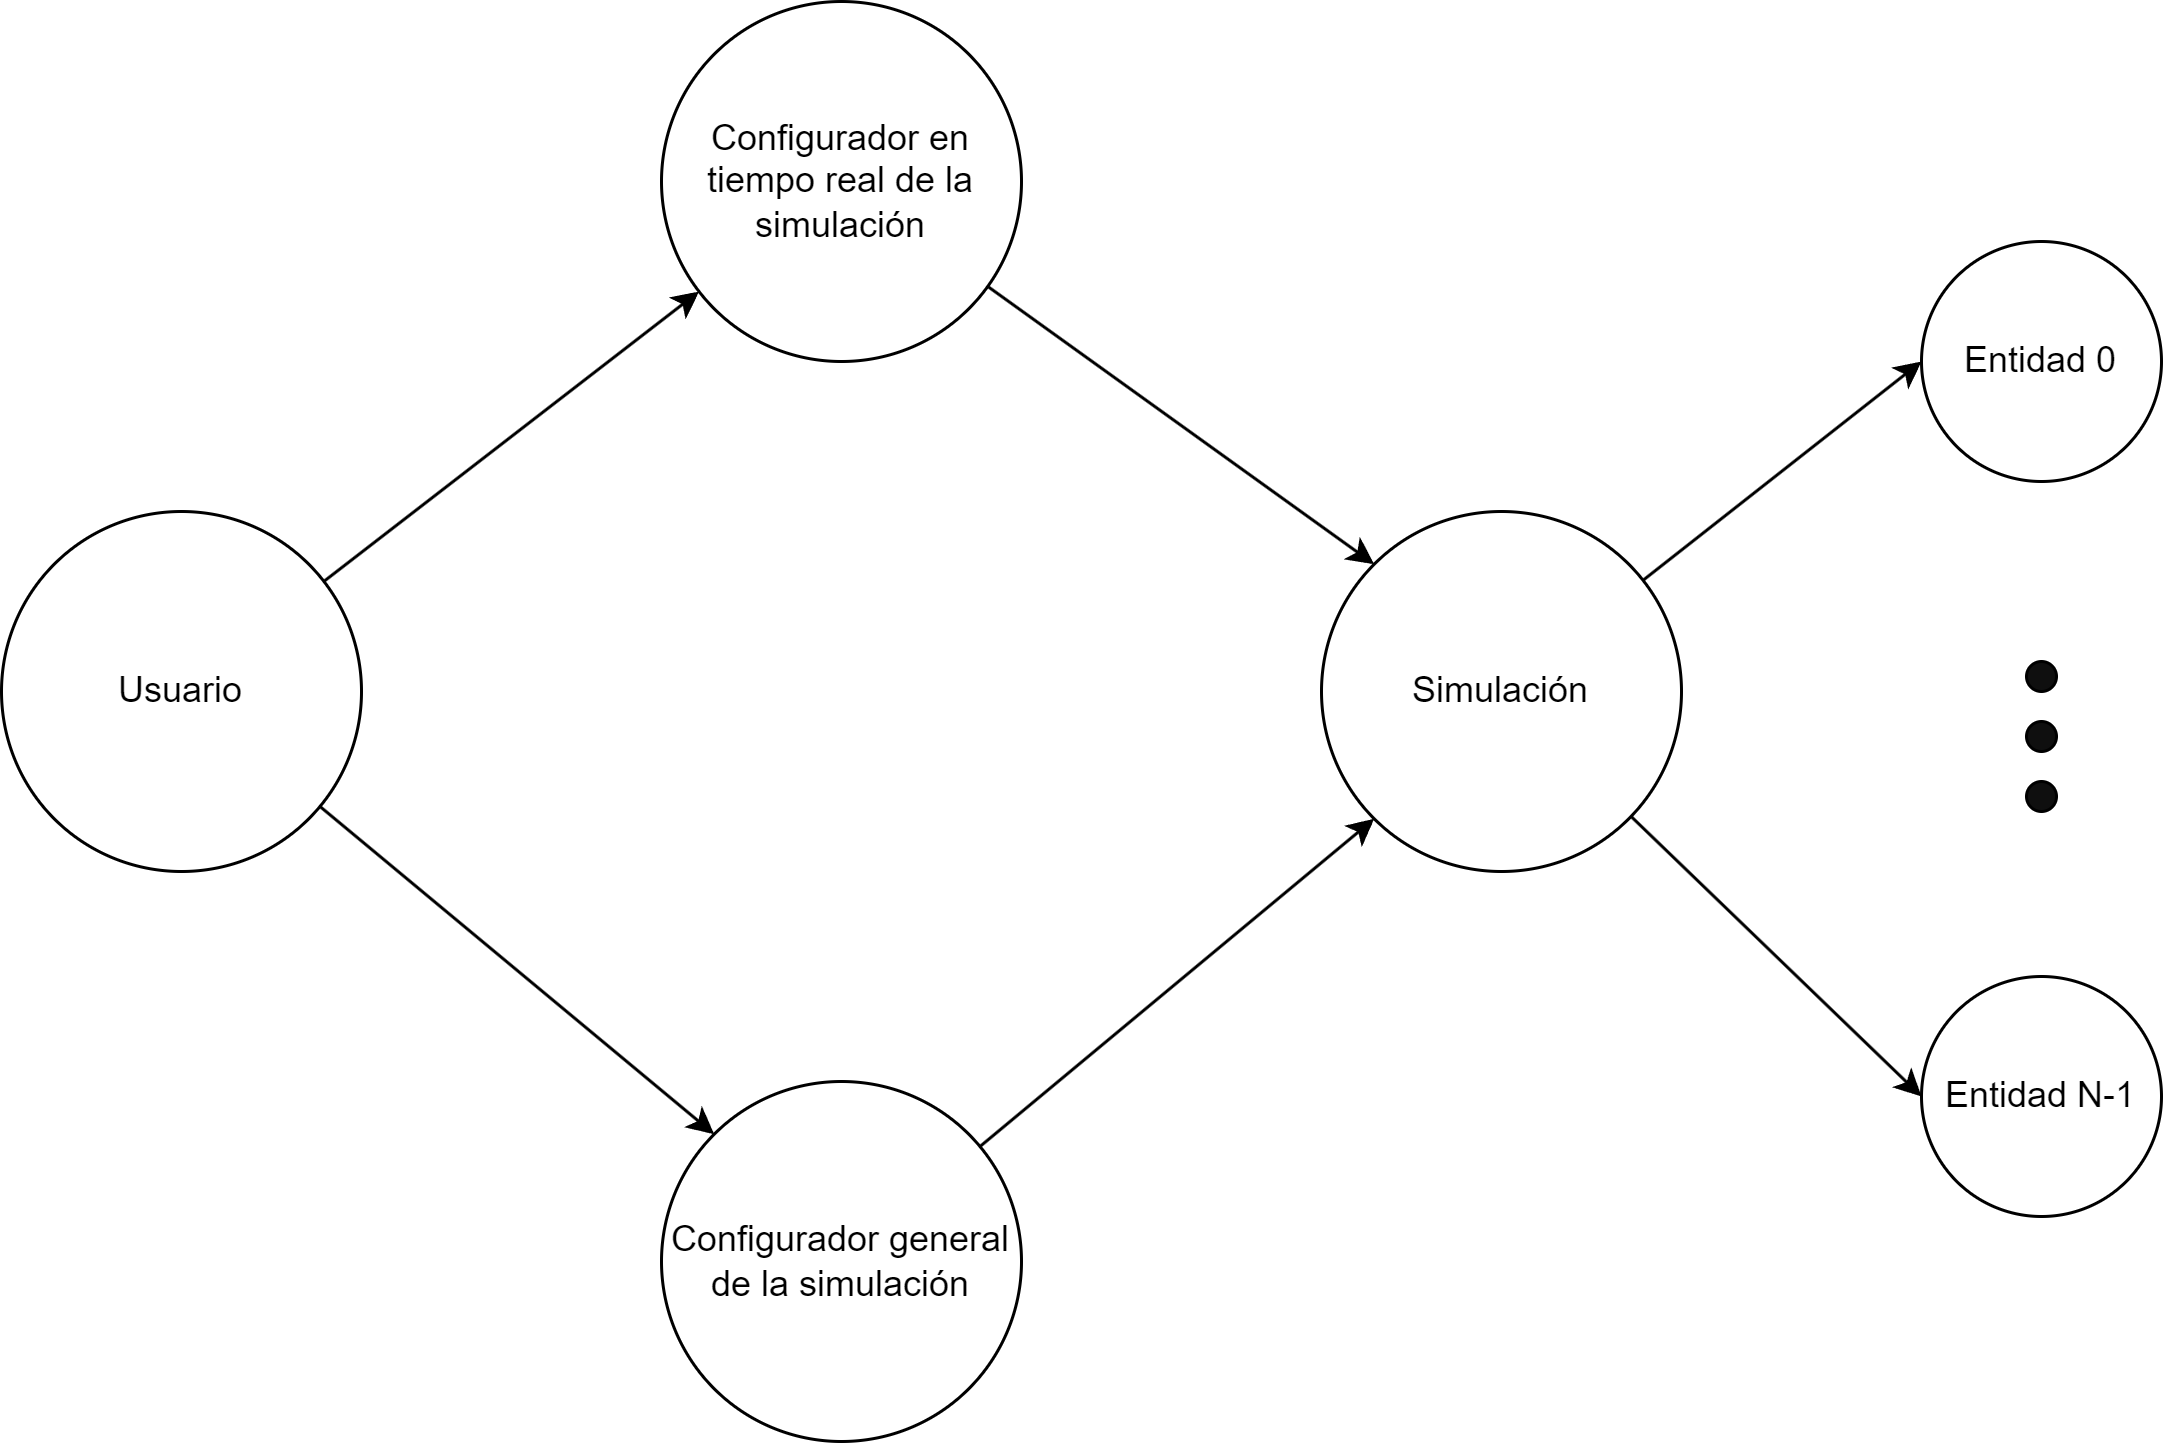
\includegraphics[width=0.8\textwidth]{imagenes/grafo-sistema.drawio.png}
    \caption{Grafo de los distintos componentes del sistema.}
 \end{figure}

El software se diseñará como una aplicación gráfica que permitirá a los usuarios simular carreras de coches, permitiendo configurar parámetros antes de la simulación y durante la carrera. El sistema recopilará información sobre la situación de carrera de cada piloto, y utilizará estos datos para simular el desempeño de cada uno en tiempo real.

\bigskip

Los usuarios interactuarán con el sistema a través de una interfaz gráfica con la que podrán modificar todos los ajustes que estimen convenientes.

\bigskip

Además, será un sistema independiente, al no necesitar interactuar con otros sistemas externos.

\subsection{Funciones del producto}

Las funciones principales de la aplicación son las siguientes:

\begin{itemize}
    \item 
    %Configuración de los parámetros antes de la carrera: 
    % Otorgará la posibilidad de 
    Configurar las distintas opciones antes de la carrera como: número de pilotos, aptitudes de cada uno, tipo de vehículo, velocidad máxima y número de vueltas. 
    
    \item Calcular el estado del piloto según las condiciones actuales de la carrera, de manera que si su estado empeora, cometerá más errores y si mejora, cometerá menos errores, todo en tiempo real.
    
    \item Modificar el estado de los pilotos durante la carrera, con independencia de las condiciones de la misma, pudiendo ver en tiempo real como afecta el cambio producido.
\end{itemize}

Y tendrá otras funciones como:

\begin{itemize}
    \item Pausar la simulación.
    \item Acelerar o reducir la velocidad de simulación.
    \item Cambiar la hora del día.
\end{itemize}

\subsection{Características de los usuarios}

Es recomendable que los usuarios tengan conocimientos básicos de informática, pero no es necesario que sepan como funcionan las carreras, ya que el proceso se encuentra automatizado. 

\subsection{Restricciones}

Las restricciones que tendrá la aplicación son las siguientes:

\begin{itemize}
    \item \textbf{RES1.-} Para el apartado gráfico y la interfaz, se utilizará el motor gráfico \textit{Unreal Engine}.
    \item \textbf{RES2.-} Una vez pausada la simulación, no se podrá modificar su velocidad.
    \item \textbf{RES3.-} El número de pilotos en la carrera no puede ser menor o igual a 1.
    \item \textbf{RES4.-} Las aptitudes de cada piloto antes de la carrera tienen que ser mayores que 0.
    % \item \textbf{RES5.-} La velocidad máxima no podrá ser menor de 150 km/h.
\end{itemize}

\subsection{Suposiciones y dependencias}

% Los requisitos descritos pueden estar sujetos a cambios en función de la evolución del proyecto y la posible adición de nuevas funcionalidades. 

% \bigskip

Este sistema funciona de forma independiente, por lo que no es necesario comunicarse con otros sistemas externos o instalar ningún programa adicional, excepto el propio simulador.

\bigskip

También se asume que el sistema operativo instalado es Windows en sus versiones 10 u 11.

\subsection{Requisitos específicos}

\subsubsection{Requisitos funcionales}

\begin{itemize}
    \item \textbf{RF1.- Modificación de parámetros antes de la carrera:} El sistema debe permitir modificar los parámetros antes de ejecutar la simulación.
    \item \textbf{RF2.- Visualización del estado de los pilotos:} El usuario podrá ver el estado de cada piloto durante la carrera, para poder realizar operaciones sobre el mismo, si lo ve necesario.
    \item \textbf{RF3.- Modificación del estado de los pilotos durante la carrera:} El sistema permitirá modificar el estado de los pilotos en tiempo real.
    \item \textbf{RF4.- Actualización de la velocidad de simulación:} El sistema permitirá actualizar la velocidad entre varias opciones predefinidas.
    \item \textbf{RF5.- Pausado y reanudado de la simulación:} El sistema permitirá pausar y reanudar la simulación que está en curso.
    \item \textbf{RF6.- Características del simulador:} El sistema debe simular la conducción de varios pilotos en una carrera de coches, como adelantamientos y sorteo de obstáculos, entre otros. Los pilotos tendrán un conjunto de condiciones que variarán durante la carrera y que afectarán a su rendimiento.
    \item \textbf{RF7.- Exportación de la configuración de la simulación:} El sistema permitirá almacenar la configuración de la carrera en un fichero para su posterior importación.
    \item \textbf{RF8.- Importación de la configuración de la simulación:} El sistema permitirá importar la configuración de la simulación.
    \item \textbf{RF9.- Visualización de la vuelta actual:} El sistema deberá realizar el cálculo y la visualización de la vuelta actual.
    \item \textbf{RF10.- Salida de la simulación en curso: }El sistema permitirá salir de la simulación que haya en ejecución al configurador.
\end{itemize}


\subsubsection{Requisitos de soporte}

\begin{itemize}
    % \item RNF1.- El sistema debe ser ejecutado en un entorno Windows 10 o Windows 11.
    \item \textbf{RNF1.-} El sistema se ejecutará en los sistemas operativos Windows 10 y Windows 11.
\end{itemize}

\subsubsection{Requisitos de usabilidad}

\begin{itemize}
    \item \textbf{RNF2.-} La interfaz deberá ser fácil de usar e intuitiva para los usuarios, de manera que puedan navegar por la misma sin demasiada dificultad.
    \item \textbf{RNF3.-} El tamaño del texto y el estilo de fuente deben ser adecuados para facilitar su lectura.
\end{itemize}

\subsubsection{Requisitos de rendimiento}

\begin{itemize}
    \item \textbf{RNF4.-} El sistema deberá tardar, como máximo, 50 milisegundos (unos 20 FPS) en ejecutar cada paso de la simulación.
    \item \textbf{RNF5.-} El cambio manual del estado de un piloto debe ser reflejado en la simulación en menos de 10 segundos.
\end{itemize}

\subsubsection{Requisitos de información del sistema}

\begin{itemize}
    \item \textbf{RI1.- Datos de los pilotos:} Nombre, nacionalidad, aguante mental y físico, agresividad y experiencia.
    % \begin{itemize}
    %     \item Nombre
    %     \item Nacionalidad
    %     \item Aguante mental
    %     \item Aguante físico
    %     \item Agresividad
    %     \item Experiencia
    % \end{itemize}
    \item \textbf{RI2.- Datos del simulador:} Velocidad de simulación, hora actual, número de vueltas, vuelta actual y número de vehículos.
\end{itemize}

\subsubsection{Aspectos legales}

La simulación no va a guardar ningún tipo de dato privado ni asociable a un individuo, haciendo que todos los datos sean anónimos. Por tanto, no es necesario seguir ningún tipo de tratamiento especial con la información insertada en la aplicación.

\subsubsection{Interfaz de usuario}

La interfaz de usuario que se utilizará para configurar los parámetros previos a la carrera estará compuesta por varias secciones para ajustar distintos parámetros de la simulación. Además, habrá otra ventana para modificar algunas características de los pilotos y dos botones para importar y exportar la configuración.

\bigskip

Durante la carrera, la interfaz de usuario tendrá un aspecto similar al de las carreras reales, con un contador de vueltas y la posición de los pilotos a la izquierda. Asimismo, se podrá pulsar sobre un piloto para ver y modificar su estado en tiempo real.

\newpage

Los bocetos de dichas interfaces son las siguientes:
% La estructura que tendrá la interfaz de usuario es la siguiente:

\begin{figure}[H]
    \centering
    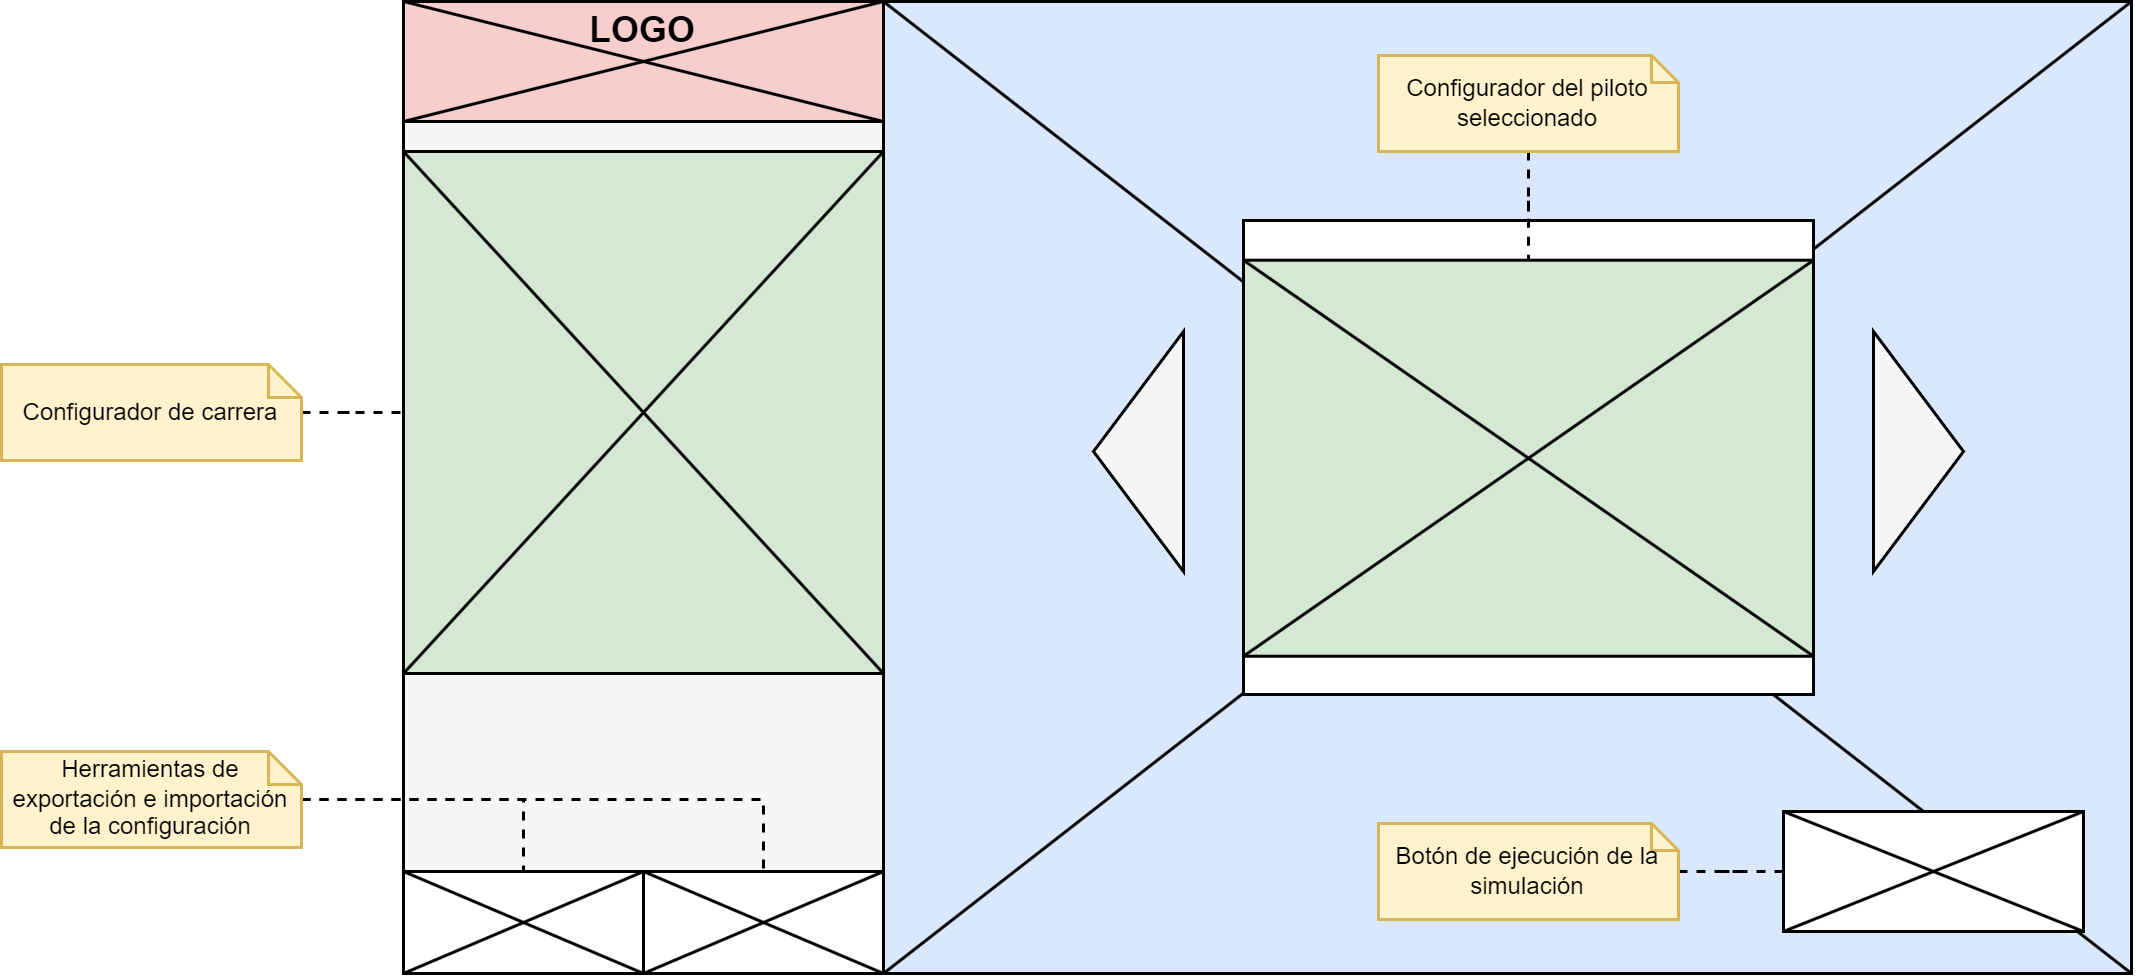
\includegraphics[width=\textwidth]{imagenes/pag1-proto.png}
    \caption{Prototipo del configurador antes de la carrera.}
    \label{fig:protoconfig}
 \end{figure}

 \begin{figure}[H]
    \centering
    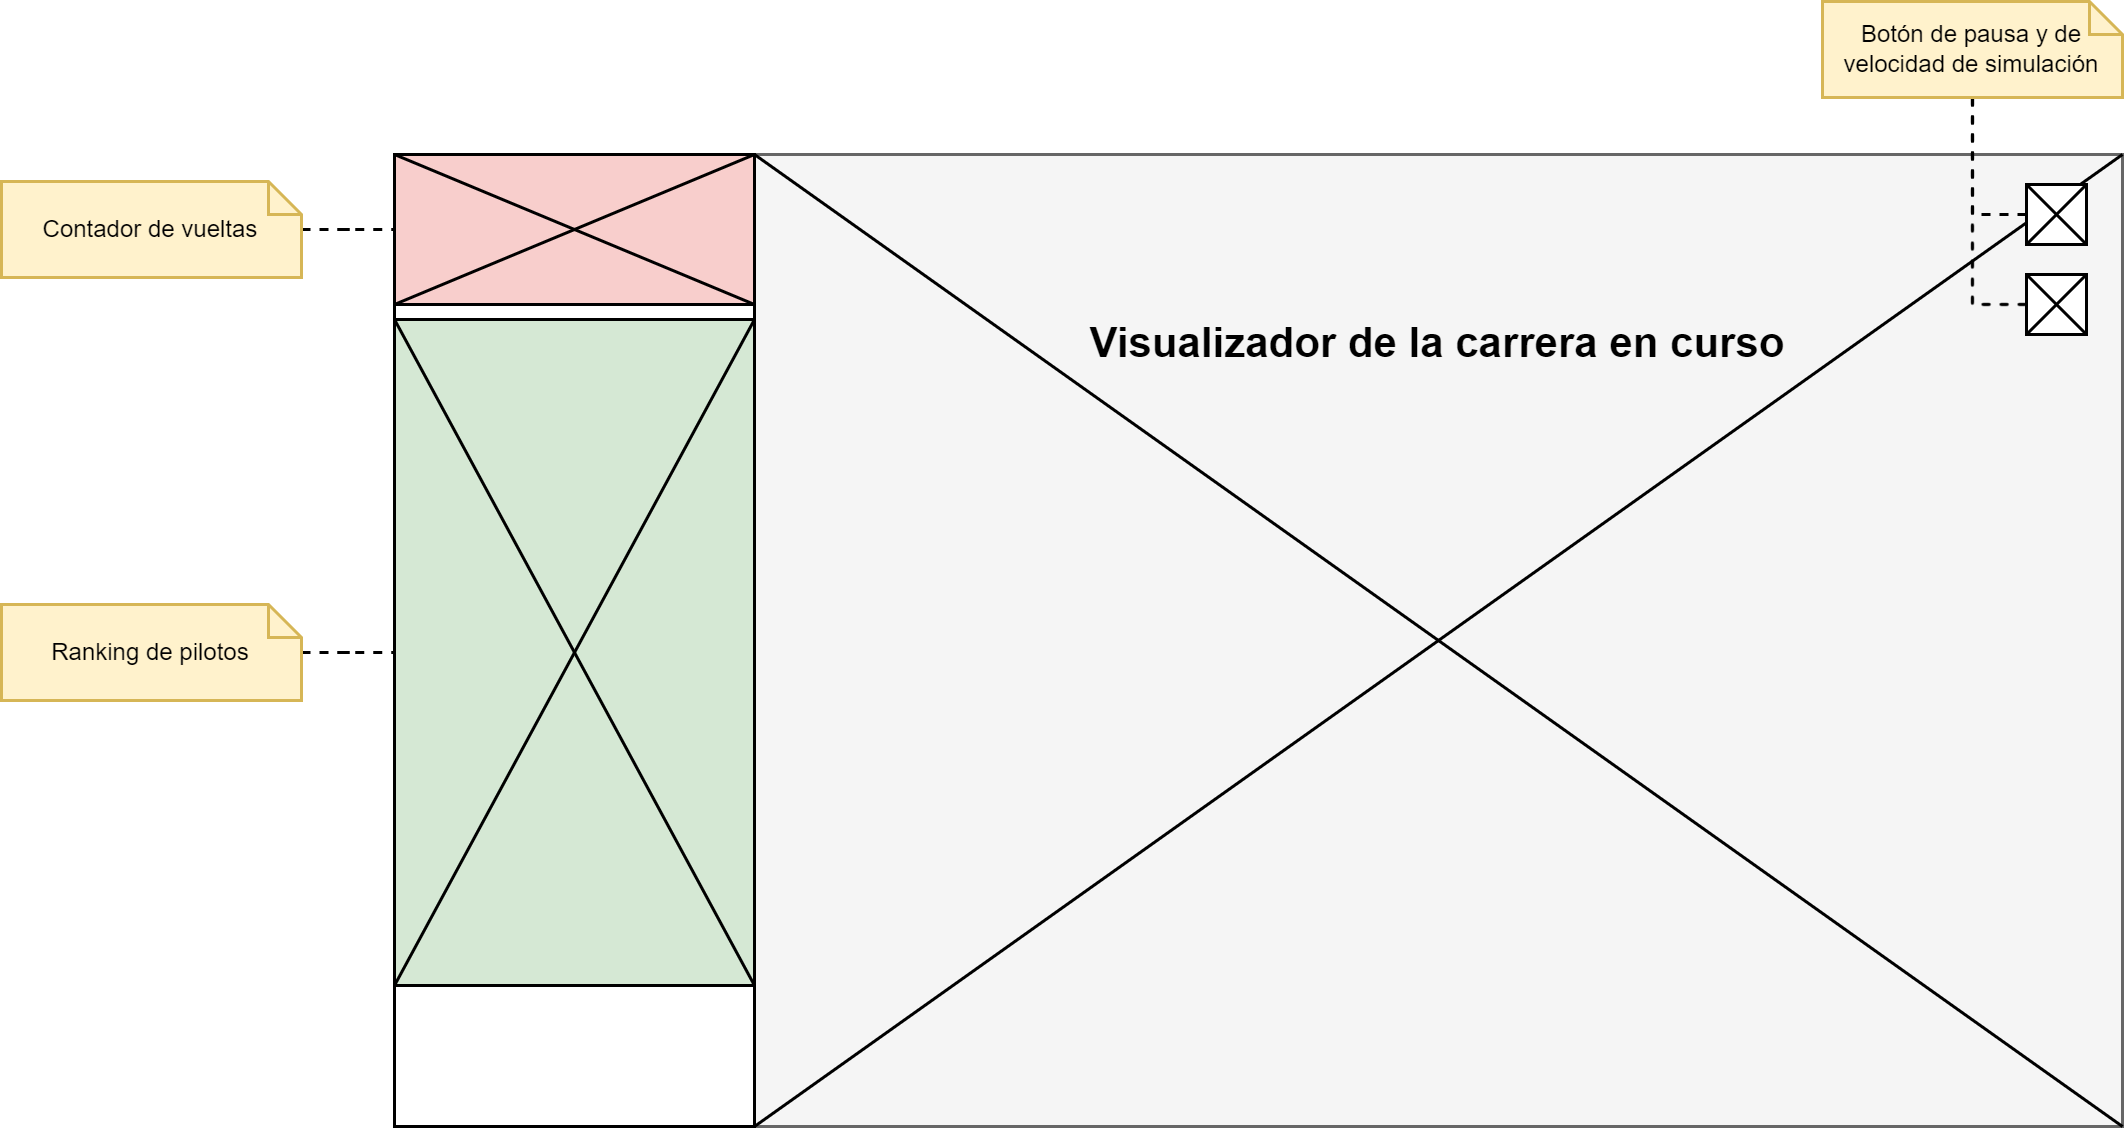
\includegraphics[width=\textwidth]{imagenes/pag2-proto.png}
    \caption{Prototipo de la interfaz de las opciones durante la carrera.}
    \label{fig:protoranking}
 \end{figure}

% % DUDAS
% PUSE EXPLICACION GENERAL, PERO NO SE EXACTAMENTE QUE ES
% esto son datos cambiantes, puedo poner algo inicial, pero seguramente haya que modificarlo al final
% no se ni siquiera el numero de sprints que va a haber!! (tendria que tener una velocidad de equipo)
\chapter{Planificación}

\section{Introducción}

Se pretende utilizar una metodología ágil para el desarrollo del proyecto, más concretamente una adaptación de Scrum a las condiciones del mismo, junto a otras herramientas.

\bigskip
% El principal motivo de adaptar Scrum es que
% rescribir
Al ser solo una persona desarrollando el proyecto, es imposible seguir algunas fases del marco de trabajo como \textit{Daily Meetings}, entre otros. Las fases que son aplicables son: \textit{Sprint Planning}. No obstante, todos los artefactos se pueden generar.

\bigskip

Otros aspectos de Scrum que se van a aplicar son: la utilización de sprints para desarrollar el proyecto, su enfoque iterativo e incremental y las Historias de Usuario.

\bigskip

Además, se van a utilizar herramientas que no son estrictamente de metodologías ágiles, como el diagrama de Gantt, para planificar la cantidad de tiempo que se piensa dedicar a cada sprint o Historia de Usuario, dependiendo del nivel de detalle. 

\bigskip

Por último, cabe recordar que no se pretende seguir Scrum de manera precisa, al no cumplir todos los requisitos para poder usarlo. Solo que se piensa usar algunos aspectos aplicables del marco, junto a otras herramientas que no son exactamente de metodologías ágiles.


\section{Product Backlog}

El \textit{Product Backlog} con las Historias de Usuario, ordenadas por prioridad y con sus Puntos de Historia (PH), son:

\begin{table}[H]
    \centering
    \begin{tabularx}{\textwidth}{| >{\centering\arraybackslash}X | >{\centering\arraybackslash}m{5.5cm} | >{\centering\arraybackslash}X | >{\centering\arraybackslash}X |}
        \hline
        \textbf{Código} & \textbf{Descripción} & \textbf{Prioridad} & \textbf{PH} \\
        \hline
        HU1 & Como usuario, quiero que el sistema simula la conducción de varios pilotos en una carrera de coches, simulando adelantamientos y sorteo de obstáculos. & 1 & 5 \\
        \hline
        HU2 & Como usuario, quiero modificar los ajustes de la simulación antes de comenzar la carrera. & 2 & 3 \\
        \hline
        HU3 & Como usuario, quiero modificar el estado de los pilotos durante la carrera. & 2 & 2 \\
        \hline
        HU4 & Como usuario, quiero ver la posición actual de los pilotos de la carrera en curso. & 3 & 3 \\
        \hline
        HU5 & Como usuario, quiero ver el número de vueltas de la carrera en curso. & 3 & 2 \\ 
        \hline
        HU6 & Como usuario, quiero guardar la configuración de una carrera para su posterior uso. & 4 & 2\\
        \hline
        HU7 & Como usuario, quiero cargar la configuración de una carrera almacenada en un archivo. & 4 & 2 \\
        \hline
        HU8 & Como usuario, quiero pausar y reanudar la simulación en curso. & 5 & 0,5 \\
        \hline
        HU9 & Como usuario, quiero modificar la velocidad de la simulación. & 5 & 0,5 \\
        \hline
    \end{tabularx}
\end{table}
    
\section{Velocidad del equipo}

Esto solo es una estimación de la velocidad que se puede alcanzar para el primer Sprint, en función de los puntos de historia realizados al final del mismo se actualizará la velocidad del equipo.

\bigskip

Algunos aspectos a tener en cuenta son:

\begin{itemize}
    \item Duración de los sprints de \sprintLength, que equivalen a \actualSprintLength, quitando fines de semana.
    \item 1 PH representa un día de trabajo ideal a jornada completa (8 horas), pero suponiendo factores externos serán 5 
    horas reales. Usando las horas reales, 1 PH se completaría en 1,6 días.
    % \item Trabajaré 24 horas semanales.
    \item Hay un total de \projectph en el proyecto.
\end{itemize}

\bigskip

Sabiendo esto, la estimación de la velocidad del equipo para la primera iteración es: $\frac{10 \text{ días/sprint}}{1.6 \text{ días/PH}} = 6.25 \text{ PH/sprint} \simeq \mathbf{7\,PH/sprint}$
% $2 \text{ semanas/sprint} \times 20 \text{ horas/semana} \times 8 \text{ horas/PH} = $

\section{Diseño del Sprint}

Este proyecto se dividirá en \sprintNro sprints, cuya duración será de \sprintLength. A continuación se desglosará qué se realizará en cada uno de ellos.

\subsection{Sprint 1}
\begin{itemize}
    \item Explicación: En este sprint se pretende tener la base de la aplicación en funcionamiento. Como base se entiende a que los coches puedan moverse por el mapa mediante el algoritmo de navegación, pudiendo esquivar obstáculos y adelantarse.
    \item Temporización:
    \item Historias de Usuario abordadas: HU1
\end{itemize}

\section{Diagrama de Gantt}

% \chapter{Análisis}

En este capítulo se abordará en más detalle cada Historia de Usuario, indicando sus pruebas de validación y las tareas que pueden surgir de cada una de ellas.

\bigskip

Cabe destacar que el campo de ``Entrega'' indica en qué sprint se va a realizar, mientras que el campo de ``Estimación'' indica cuanto Puntos de Historia (PH) se le han asignado.

\bigskip

Cada Historia de Usuario se desarrollará en una tabla a continuación:

% \section{Historias de Usuario divididas en subtareas}



% \begin{table}[H]
%     \begin{tabularx}{\textwidth}{| X | X | X |}
%         \hline
%         \multicolumn{1}{|l|}{\textbf{Identificador:} HU1} & \multicolumn{2}{l|}{Algoritmo de navegación.}
%         \\ \hline
%         \multicolumn{3}{|>{\hsize=\dimexpr3\hsize+4\tabcolsep+2\arrayrulewidth\relax\linewidth=\hsize}X|}{\textbf{Descripción:} Como usuario, quiero que el sistema simule la conducción de varios pilotos en una carrera de coches, incluyendo adelantamientos y sorteo de obstáculos.}
%         \\ \hline
%         \textbf{Estimación:} 5 & \textbf{Prioridad:} 1 & \textbf{Entrega:} 1
%         \\ \hline
%         \multicolumn{3}{|>{\hsize=\dimexpr3\hsize+4\tabcolsep+2\arrayrulewidth\relax\linewidth=\hsize}X|}{\textbf{Tareas:}
%         \begin{itemize}
%             \item Implementar el controlador del volante de los vehículos, de manera que sean capaces de seguir una ruta de forma suave.
%             \item Implementar la malla de navegación.
%             \item Implementar el algoritmo a partir de la malla.
%             \item Implementar la lógica de los vehículos, de forma que sean capaces usar esta malla para tomar decisiones.
%         \end{itemize}
%         }
%         \\ \hline
%         \multicolumn{3}{|>{\hsize=\dimexpr3\hsize+4\tabcolsep+2\arrayrulewidth\relax\linewidth=\hsize}X|}{\textbf{Requisitos relacionados:} RF6, RNF4.}
%         \\ \hline
%         \multicolumn{3}{|>{\hsize=\dimexpr3\hsize+4\tabcolsep+2\arrayrulewidth\relax\linewidth=\hsize}X|}{\textbf{Pruebas de aceptación:}
%         \begin{itemize}
%             \item Los pilotos deben ser capaces de esquivar obstáculos en la pista.
%             \item La simulación debe poder ejecutarse en un tiempo razonable, de manera que se pueda seguir la carrera en tiempo real.
%             \item Los pilotos deben ser capaces de adelantar a otros que sean más lentos sin provocar accidentes.
%         \end{itemize}
%         }
%         \\ \hline
%         \multicolumn{3}{|>{\hsize=\dimexpr3\hsize+4\tabcolsep+2\arrayrulewidth\relax\linewidth=\hsize}X|}{\textbf{Observaciones:}}
%         \\ \hline
%     \end{tabularx}
% \end{table}

% \begin{table}[H]
%     \begin{tabularx}{\textwidth}{| X | X | X |}
%         \hline
%         \multicolumn{1}{|l|}{\textbf{Identificador:} HU1} & \multicolumn{2}{l|}{lorem ipsum dolor sit amet.}
%         \\ \hline
%         \multicolumn{3}{|>{\hsize=\dimexpr3\hsize+4\tabcolsep+2\arrayrulewidth\relax\linewidth=\hsize}X|}{\textbf{Descripción:} lorem ipsum dolor sit amet.}
%         \\ \hline
%         \textbf{Estimación:} X & \textbf{Prioridad:} X & \textbf{Entrega:} X
%         \\ \hline
%         \multicolumn{3}{|>{\hsize=\dimexpr3\hsize+4\tabcolsep+2\arrayrulewidth\relax\linewidth=\hsize}X|}{\textbf{Tareas:}
%         \begin{itemize}
%             \item Roma no se hizo en un día.
%         \end{itemize}
%         }
%         \\ \hline
%         \multicolumn{3}{|>{\hsize=\dimexpr3\hsize+4\tabcolsep+2\arrayrulewidth\relax\linewidth=\hsize}X|}{\textbf{Requisitos relacionados:} RF6, RNF4.}
%         \\ \hline
%         \multicolumn{3}{|>{\hsize=\dimexpr3\hsize+4\tabcolsep+2\arrayrulewidth\relax\linewidth=\hsize}X|}{\textbf{Pruebas de aceptación:}
%         \begin{itemize}
%             \item Algo tangible.
%         \end{itemize}
%         }
%         \\ \hline
%         \multicolumn{3}{|>{\hsize=\dimexpr3\hsize+4\tabcolsep+2\arrayrulewidth\relax\linewidth=\hsize}X|}{\textbf{Observaciones:}}
%         \\ \hline
%     \end{tabularx}
% \end{table}

\begin{table}[H]
    \begin{tabularx}{\textwidth}{| X | X | X |}
        \hline
        \multicolumn{1}{|l|}{\textbf{Identificador:} HU1} & \multicolumn{2}{l|}{Modelado de los coches y circuito.}
        \\ \hline
        \multicolumn{3}{|>{\hsize=\dimexpr3\hsize+4\tabcolsep+2\arrayrulewidth\relax\linewidth=\hsize}X|}{\textbf{Descripción:} Como usuario, quiero tener una representación en 3D de los coches y el circuito.}
        \\ \hline
        \textbf{Estimación:} 3 & \textbf{Prioridad:} 1 & \textbf{Entrega:} 4
        \\ \hline
        \multicolumn{3}{|>{\hsize=\dimexpr3\hsize+4\tabcolsep+2\arrayrulewidth\relax\linewidth=\hsize}X|}{\textbf{Tareas:}
        \begin{itemize}
            \item Modelar el trazado del circuito.
            \item Modelar los vehículos, o en su defecto, obtener modelos ya hechos.
        \end{itemize}
        }
        \\ \hline
        \multicolumn{3}{|>{\hsize=\dimexpr3\hsize+4\tabcolsep+2\arrayrulewidth\relax\linewidth=\hsize}X|}{\textbf{Requisitos relacionados:}}
        \\ \hline
        \multicolumn{3}{|>{\hsize=\dimexpr3\hsize+4\tabcolsep+2\arrayrulewidth\relax\linewidth=\hsize}X|}{\textbf{Pruebas de aceptación:}
        }
        \\ \hline
        \multicolumn{3}{|>{\hsize=\dimexpr3\hsize+4\tabcolsep+2\arrayrulewidth\relax\linewidth=\hsize}X|}{\textbf{Observaciones:}}
        \\ \hline
    \end{tabularx}
\end{table}

\begin{table}[H]
    \begin{tabularx}{\textwidth}{| X | X | X |}
        \hline
        \multicolumn{1}{|l|}{\textbf{Identificador:} HU2} & \multicolumn{2}{l|}{Cálculo de ruta óptima en el circuito.}
        \\ \hline
        \multicolumn{3}{|>{\hsize=\dimexpr3\hsize+4\tabcolsep+2\arrayrulewidth\relax\linewidth=\hsize}X|}{\textbf{Descripción:} Como usuario, quiero que los pilotos calculen la ruta más óptima en el circuito.}
        \\ \hline
        \textbf{Estimación:} 8 & \textbf{Prioridad:} 1 & \textbf{Entrega:} 5
        \\ \hline
        \multicolumn{3}{|>{\hsize=\dimexpr3\hsize+4\tabcolsep+2\arrayrulewidth\relax\linewidth=\hsize}X|}{\textbf{Tareas:}
        \begin{itemize}
            \item Implementar la malla de navegación, para que los coches puedan calcular rutas.
            \item Implementar el algoritmo de navegación, que haga uso de la malla.
            \item Crear los objetos auxiliares, para indicar a la malla la ruta más rápida.
        \end{itemize}
        }
        \\ \hline
        \multicolumn{3}{|>{\hsize=\dimexpr3\hsize+4\tabcolsep+2\arrayrulewidth\relax\linewidth=\hsize}X|}{\textbf{Requisitos relacionados:} RF6, RNF4.}
        \\ \hline
        \multicolumn{3}{|>{\hsize=\dimexpr3\hsize+4\tabcolsep+2\arrayrulewidth\relax\linewidth=\hsize}X|}{\textbf{Pruebas de aceptación:}
        \begin{itemize}
            \item El algoritmo debe calcular una ruta que no dé la vuelta en el circuito.
            \item El algoritmo debe obtener un resultado en un tiempo razonable.
        \end{itemize}
        }
        \\ \hline
        \multicolumn{3}{|>{\hsize=\dimexpr3\hsize+4\tabcolsep+2\arrayrulewidth\relax\linewidth=\hsize}X|}{\textbf{Observaciones:}}
        \\ \hline
    \end{tabularx}
\end{table}

\begin{table}[H]
    \begin{tabularx}{\textwidth}{| X | X | X |}
        \hline
        \multicolumn{1}{|l|}{\textbf{Identificador:} HU3} & \multicolumn{2}{l|}{Seguimiento de una ruta con el volante.}
        \\ \hline
        \multicolumn{3}{|>{\hsize=\dimexpr3\hsize+4\tabcolsep+2\arrayrulewidth\relax\linewidth=\hsize}X|}{\textbf{Descripción:} Como usuario, quiero que los pilotos sean capaces de seguir una ruta de manera suave.}
        \\ \hline
        \textbf{Estimación:} 5 & \textbf{Prioridad:} 1 & \textbf{Entrega:} 4
        \\ \hline
        \multicolumn{3}{|>{\hsize=\dimexpr3\hsize+4\tabcolsep+2\arrayrulewidth\relax\linewidth=\hsize}X|}{\textbf{Tareas:}
        \begin{itemize}
            \item Implementar el controlador PID para usarlo en el volante.
            \item Implementar un algoritmo para obtener el mejor valor de las constantes.
        \end{itemize}
        }
        \\ \hline
        \multicolumn{3}{|>{\hsize=\dimexpr3\hsize+4\tabcolsep+2\arrayrulewidth\relax\linewidth=\hsize}X|}{\textbf{Requisitos relacionados:} RF6, RNF4.}
        \\ \hline
        \multicolumn{3}{|>{\hsize=\dimexpr3\hsize+4\tabcolsep+2\arrayrulewidth\relax\linewidth=\hsize}X|}{\textbf{Dependencias:} HU2.}
        \\ \hline   
        \multicolumn{3}{|>{\hsize=\dimexpr3\hsize+4\tabcolsep+2\arrayrulewidth\relax\linewidth=\hsize}X|}{\textbf{Pruebas de aceptación:}
        \begin{itemize}
            \item La amplitud de las oscilaciones del vehículo en línea recta deben tener un tamaño menor a la anchura del coche.
            \item El coche debe tomar la curvas de manera suave.
        \end{itemize}
        }
        \\ \hline
        \multicolumn{3}{|>{\hsize=\dimexpr3\hsize+4\tabcolsep+2\arrayrulewidth\relax\linewidth=\hsize}X|}{\textbf{Observaciones:} El algoritmo utilizado para ajustar los valores del PID ha sido un algoritmo genético.}
        \\ \hline
    \end{tabularx}
\end{table}

\begin{table}[H]
    \begin{tabularx}{\textwidth}{| X | X | X |}
        \hline
        \multicolumn{1}{|l|}{\textbf{Identificador:} HU4} & \multicolumn{2}{l|}{Adelantamiento entre vehículos.}
        \\ \hline
        \multicolumn{3}{|>{\hsize=\dimexpr3\hsize+4\tabcolsep+2\arrayrulewidth\relax\linewidth=\hsize}X|}{\textbf{Descripción:} Como usuario, quiero que los pilotos sean capaces de adelantarse entre ellos.}
        \\ \hline
        \textbf{Estimación:} 5 & \textbf{Prioridad:} 1 & \textbf{Entrega:} 6
        \\ \hline
        \multicolumn{3}{|>{\hsize=\dimexpr3\hsize+4\tabcolsep+2\arrayrulewidth\relax\linewidth=\hsize}X|}{\textbf{Tareas:}
        \begin{itemize}
            \item Haciendo uso del algoritmo de HU2, implementar la lógica necesaria para saber cuando recalcular la ruta.
            \item Ajustar las colisiones de los vehículos, de forma que tengan espacio para adelantar.
        \end{itemize}
        }
        \\ \hline
        \multicolumn{3}{|>{\hsize=\dimexpr3\hsize+4\tabcolsep+2\arrayrulewidth\relax\linewidth=\hsize}X|}{\textbf{Requisitos relacionados:} RF6, RNF4.}
        \\ \hline
        \multicolumn{3}{|>{\hsize=\dimexpr3\hsize+4\tabcolsep+2\arrayrulewidth\relax\linewidth=\hsize}X|}{\textbf{Dependencias:} HU2.}
        \\ \hline   
        \multicolumn{3}{|>{\hsize=\dimexpr3\hsize+4\tabcolsep+2\arrayrulewidth\relax\linewidth=\hsize}X|}{\textbf{Pruebas de aceptación:}
        \begin{itemize}
            \item El adelantamiento de un coche a otro no debe provocar el accidente de ninguno de los dos.
        \end{itemize}
        }
        \\ \hline
        \multicolumn{3}{|>{\hsize=\dimexpr3\hsize+4\tabcolsep+2\arrayrulewidth\relax\linewidth=\hsize}X|}{\textbf{Observaciones:}}
        \\ \hline
    \end{tabularx}
\end{table}

\begin{table}[H]
    \begin{tabularx}{\textwidth}{| X | X | X |}
        \hline
        \multicolumn{1}{|l|}{\textbf{Identificador:} HU5} & \multicolumn{2}{l|}{Maniobra de recuperación en accidentes.}
        \\ \hline
        \multicolumn{3}{|>{\hsize=\dimexpr3\hsize+4\tabcolsep+2\arrayrulewidth\relax\linewidth=\hsize}X|}{\textbf{Descripción:} Como usuario, quiero que los pilotos sean capaces de recuperarse después de un accidente.}
        \\ \hline
        \textbf{Estimación:} 3 & \textbf{Prioridad:} 1 & \textbf{Entrega:} 6
        \\ \hline
        \multicolumn{3}{|>{\hsize=\dimexpr3\hsize+4\tabcolsep+2\arrayrulewidth\relax\linewidth=\hsize}X|}{\textbf{Tareas:}
        \begin{itemize}
            \item Implementar la lógica para que los pilotos recalculen una ruta que les devuelva a la pista utilizando el algoritmo de navegación.
        \end{itemize}
        }
        \\ \hline
        \multicolumn{3}{|>{\hsize=\dimexpr3\hsize+4\tabcolsep+2\arrayrulewidth\relax\linewidth=\hsize}X|}{\textbf{Requisitos relacionados:} RF6, RNF4.}
        \\ \hline
        \multicolumn{3}{|>{\hsize=\dimexpr3\hsize+4\tabcolsep+2\arrayrulewidth\relax\linewidth=\hsize}X|}{\textbf{Dependencias:} HU2.}
        \\ \hline        
        \multicolumn{3}{|>{\hsize=\dimexpr3\hsize+4\tabcolsep+2\arrayrulewidth\relax\linewidth=\hsize}X|}{\textbf{Pruebas de aceptación:}
        \begin{itemize}
            \item La nueva ruta debe calcularse en un tiempo razonable, de manera que pueda hacerse en tiempo real.
        \end{itemize}
        }
        \\ \hline
        \multicolumn{3}{|>{\hsize=\dimexpr3\hsize+4\tabcolsep+2\arrayrulewidth\relax\linewidth=\hsize}X|}{\textbf{Observaciones:}}
        \\ \hline
    \end{tabularx}
\end{table}

% ANTIGUOS DEL SPRINT 4

\begin{table}[H]
    \begin{tabularx}{\textwidth}{| X | X | X |}
        \hline
        \multicolumn{1}{|l|}{\textbf{Identificador:} HU6} & \multicolumn{2}{l|}{Modificación de ajustes antes de la carrera.}
        \\ \hline
        \multicolumn{3}{|>{\hsize=\dimexpr3\hsize+4\tabcolsep+2\arrayrulewidth\relax\linewidth=\hsize}X|}{\textbf{Descripción:} Como usuario, quiero modificar los ajustes de la simulación antes de comenzar la carrera.}
        \\ \hline
        \textbf{Estimación:} 2 & \textbf{Prioridad:} 2 & \textbf{Entrega:} 7
        \\ \hline
        \multicolumn{3}{|>{\hsize=\dimexpr3\hsize+4\tabcolsep+2\arrayrulewidth\relax\linewidth=\hsize}X|}{\textbf{Tareas:}
        \begin{itemize}
            \item Implementar los deslizadores correspondientes al número de vueltas, de coches, hora, aguante y experiencia.
            \item Implementar los campos de texto para el nombre y los apellidos.
            \item Programar la lógica necesaria para que los coches aparezcan en las posiciones correctas.
            \item Programar la lógica de las flechas para elegir a los pilotos.
        \end{itemize}
        }
        \\ \hline
        \multicolumn{3}{|>{\hsize=\dimexpr3\hsize+4\tabcolsep+2\arrayrulewidth\relax\linewidth=\hsize}X|}{\textbf{Requisitos relacionados:} RF1, RNF2, RNF3.}
        \\ \hline
        \multicolumn{3}{|>{\hsize=\dimexpr3\hsize+4\tabcolsep+2\arrayrulewidth\relax\linewidth=\hsize}X|}{\textbf{Pruebas de aceptación:}
        \begin{itemize}
            % \item No se podrá elegir un número menor de 1 para la cantidad de vueltas.
            % \item No se podrá elegir un número menor de 2 coches.
            \item No se podrá dejar el campo del nombre y los apellidos vacíos.
        \end{itemize}
        }
        \\ \hline
        \multicolumn{3}{|>{\hsize=\dimexpr3\hsize+4\tabcolsep+2\arrayrulewidth\relax\linewidth=\hsize}X|}{\textbf{Observaciones:}}
        \\ \hline
    \end{tabularx}
\end{table}

\begin{table}[H]
    \begin{tabularx}{\textwidth}{| X | X | X |}
        \hline
        \multicolumn{1}{|l|}{\textbf{Identificador:} HU7} & \multicolumn{2}{l|}{Modificación del estado de los pilotos.}
        \\ \hline
        \multicolumn{3}{|>{\hsize=\dimexpr3\hsize+4\tabcolsep+2\arrayrulewidth\relax\linewidth=\hsize}X|}{\textbf{Descripción:} Como usuario, quiero modificar el estado de los pilotos durante la carrera.}
        \\ \hline
        \textbf{Estimación:} 2 & \textbf{Prioridad:} 2 & \textbf{Entrega:} 7
        \\ \hline
        \multicolumn{3}{|>{\hsize=\dimexpr3\hsize+4\tabcolsep+2\arrayrulewidth\relax\linewidth=\hsize}X|}{\textbf{Tareas:}
        \begin{itemize}
            \item Implementar los deslizadores referentes al aguante físico y mental y la agresividad.
        \end{itemize}
        }
        \\ \hline
        \multicolumn{3}{|>{\hsize=\dimexpr3\hsize+4\tabcolsep+2\arrayrulewidth\relax\linewidth=\hsize}X|}{\textbf{Requisitos relacionados:} RF3, RNF5.}
        \\ \hline
        \multicolumn{3}{|>{\hsize=\dimexpr3\hsize+4\tabcolsep+2\arrayrulewidth\relax\linewidth=\hsize}X|}{\textbf{Dependencias:} HU4.}        
        \\ \hline
        \multicolumn{3}{|>{\hsize=\dimexpr3\hsize+4\tabcolsep+2\arrayrulewidth\relax\linewidth=\hsize}X|}{\textbf{Pruebas de aceptación:}
        \begin{itemize}
            \item Los cambios en el estado deberán verse reflejados en el comportamiento del piloto seleccionado durante la carrera.
        \end{itemize}
        }
        \\ \hline
        \multicolumn{3}{|>{\hsize=\dimexpr3\hsize+4\tabcolsep+2\arrayrulewidth\relax\linewidth=\hsize}X|}{\textbf{Observaciones:}}
        \\ \hline
    \end{tabularx}
\end{table}


\begin{table}[H]
    \begin{tabularx}{\textwidth}{| X | X | X |}
        \hline
        \multicolumn{1}{|l|}{\textbf{Identificador:} HU8} & \multicolumn{2}{l|}{Visualización de la información de los pilotos.}
        \\ \hline
        \multicolumn{3}{|>{\hsize=\dimexpr3\hsize+4\tabcolsep+2\arrayrulewidth\relax\linewidth=\hsize}X|}{\textbf{Descripción:} Como usuario, quiero ver la posición actual y el estado de los pilotos de la carrera en curso.}
        \\ \hline
        \textbf{Estimación:} 3 & \textbf{Prioridad:} 3 & \textbf{Entrega:} 7
        \\ \hline
        \multicolumn{3}{|>{\hsize=\dimexpr3\hsize+4\tabcolsep+2\arrayrulewidth\relax\linewidth=\hsize}X|}{\textbf{Tareas:}
        \begin{itemize}
            \item Implementar el panel de las posiciones y el estado.
            \item Implementar la lógica asociada al cálculo de la posición general de cada piloto.
            \item Implementar la funcionalidad de mostrar los deslizadores del piloto al pulsar.
        \end{itemize}
        }
        \\ \hline
        \multicolumn{3}{|>{\hsize=\dimexpr3\hsize+4\tabcolsep+2\arrayrulewidth\relax\linewidth=\hsize}X|}{\textbf{Requisitos relacionados:} RF2, RNF3.}
        \\ \hline
        \multicolumn{3}{|>{\hsize=\dimexpr3\hsize+4\tabcolsep+2\arrayrulewidth\relax\linewidth=\hsize}X|}{\textbf{Pruebas de aceptación:}
        \begin{itemize}
            \item Cuando un piloto cambie posiciones con otro, la lista de posiciones de los pilotos debe cambiar.
            \item El cambio del estado del piloto producido por la carrera será reflejado en el deslizador.
        \end{itemize}
        }
        \\ \hline
        \multicolumn{3}{|>{\hsize=\dimexpr3\hsize+4\tabcolsep+2\arrayrulewidth\relax\linewidth=\hsize}X|}{\textbf{Observaciones:}}
        \\ \hline
    \end{tabularx}
\end{table}

\begin{table}[H]
    \begin{tabularx}{\textwidth}{| X | X | X |}
        \hline
        \multicolumn{1}{|l|}{\textbf{Identificador:} HU9} & \multicolumn{2}{l|}{Visualización de las vueltas restantes.}
        \\ \hline
        \multicolumn{3}{|>{\hsize=\dimexpr3\hsize+4\tabcolsep+2\arrayrulewidth\relax\linewidth=\hsize}X|}{\textbf{Descripción:} Como usuario, quiero ver el número de vueltas de la carrera en curso.}
        \\ \hline
        \textbf{Estimación:} 2 & \textbf{Prioridad:} 3 & \textbf{Entrega:} 8
        \\ \hline
        \multicolumn{3}{|>{\hsize=\dimexpr3\hsize+4\tabcolsep+2\arrayrulewidth\relax\linewidth=\hsize}X|}{\textbf{Tareas:}
        \begin{itemize}
            \item Implementar la lógica para calcular la vuelta actual.
            \item Crear el contador de la interfaz que mostrará las vueltas.
        \end{itemize}
        }
        \\ \hline
        \multicolumn{3}{|>{\hsize=\dimexpr3\hsize+4\tabcolsep+2\arrayrulewidth\relax\linewidth=\hsize}X|}{\textbf{Requisitos relacionados:} RF9, RNF3.}
        \\ \hline
        \multicolumn{3}{|>{\hsize=\dimexpr3\hsize+4\tabcolsep+2\arrayrulewidth\relax\linewidth=\hsize}X|}{\textbf{Pruebas de aceptación:}
        \begin{itemize}
            \item El marcador no deberá mostrar como vuelta actual el número 0 ni un número superior al número máximo.
        \end{itemize}
        }
        \\ \hline
        \multicolumn{3}{|>{\hsize=\dimexpr3\hsize+4\tabcolsep+2\arrayrulewidth\relax\linewidth=\hsize}X|}{\textbf{Observaciones:}}
        \\ \hline
    \end{tabularx}
\end{table}


\begin{table}[H]
    \begin{tabularx}{\textwidth}{| X | X | X |}
        \hline
        \multicolumn{1}{|l|}{\textbf{Identificador:} HU10} & \multicolumn{2}{l|}{Exportación de la configuración.}
        \\ \hline
        \multicolumn{3}{|>{\hsize=\dimexpr3\hsize+4\tabcolsep+2\arrayrulewidth\relax\linewidth=\hsize}X|}{\textbf{Descripción:} Como usuario, quiero guardar la configuración de una carrera para su posterior uso.}
        \\ \hline
        \textbf{Estimación:} 2 & \textbf{Prioridad:} 4 & \textbf{Entrega:} 8
        \\ \hline
        \multicolumn{3}{|>{\hsize=\dimexpr3\hsize+4\tabcolsep+2\arrayrulewidth\relax\linewidth=\hsize}X|}{\textbf{Tareas:}
        \begin{itemize}
            \item Implementar la lógica referente a la escritura de la configuración en un archivo externo.
        \end{itemize}
        }
        \\ \hline
        \multicolumn{3}{|>{\hsize=\dimexpr3\hsize+4\tabcolsep+2\arrayrulewidth\relax\linewidth=\hsize}X|}{\textbf{Requisitos relacionados:} RF7.}
        \\ \hline
        \multicolumn{3}{|>{\hsize=\dimexpr3\hsize+4\tabcolsep+2\arrayrulewidth\relax\linewidth=\hsize}X|}{\textbf{Pruebas de aceptación:}
        \begin{itemize}
            \item Al pulsar el botón se debe producir un fichero externo con la configuración exacta que había en el momento.
        \end{itemize}
        }
        \\ \hline
        \multicolumn{3}{|>{\hsize=\dimexpr3\hsize+4\tabcolsep+2\arrayrulewidth\relax\linewidth=\hsize}X|}{\textbf{Observaciones:}}
        \\ \hline
    \end{tabularx}
\end{table}

\begin{table}[H]
    \begin{tabularx}{\textwidth}{| X | X | X |}
        \hline
        \multicolumn{1}{|l|}{\textbf{Identificador:} HU11} & \multicolumn{2}{l|}{Importación de la configuración.}
        \\ \hline
        \multicolumn{3}{|>{\hsize=\dimexpr3\hsize+4\tabcolsep+2\arrayrulewidth\relax\linewidth=\hsize}X|}{\textbf{Descripción:} Como usuario, quiero cargar la configuración de una carrera almacenada en un archivo.}
        \\ \hline
        \textbf{Estimación:} 2 & \textbf{Prioridad:} 4 & \textbf{Entrega:} 8
        \\ \hline
        \multicolumn{3}{|>{\hsize=\dimexpr3\hsize+4\tabcolsep+2\arrayrulewidth\relax\linewidth=\hsize}X|}{\textbf{Tareas:}
        \begin{itemize}
            \item Implementar la lógica referente a la modificación de los parámetros por los valores que se encuentren en el archivo.
        \end{itemize}
        }
        \\ \hline
        \multicolumn{3}{|>{\hsize=\dimexpr3\hsize+4\tabcolsep+2\arrayrulewidth\relax\linewidth=\hsize}X|}{\textbf{Requisitos relacionados:} RF8.}
        \\ \hline
        \multicolumn{3}{|>{\hsize=\dimexpr3\hsize+4\tabcolsep+2\arrayrulewidth\relax\linewidth=\hsize}X|}{\textbf{Pruebas de aceptación:}
        \begin{itemize}
            % \item El fichero generado en la fase de exportación debe ser legible por la aplicación.
            \item Ante un fichero válido de configuración, la aplicación lo leerá correctamente y modificará los parámetros de forma adecuada.
        \end{itemize}
        }
        \\ \hline
        \multicolumn{3}{|>{\hsize=\dimexpr3\hsize+4\tabcolsep+2\arrayrulewidth\relax\linewidth=\hsize}X|}{\textbf{Observaciones:}}
        \\ \hline
    \end{tabularx}
\end{table}


\begin{table}[H]
    \begin{tabularx}{\textwidth}{| X | X | X |}
        \hline
        \multicolumn{1}{|l|}{\textbf{Identificador:} HU12} & \multicolumn{2}{l|}{Pausado y reanudación de la simulación.}
        \\ \hline
        \multicolumn{3}{|>{\hsize=\dimexpr3\hsize+4\tabcolsep+2\arrayrulewidth\relax\linewidth=\hsize}X|}{\textbf{Descripción:} Como usuario, quiero pausar y reanudar la simulación en curso.}
        \\ \hline
        \textbf{Estimación:} 0,5 & \textbf{Prioridad:} 5 & \textbf{Entrega:} 8
        \\ \hline
        \multicolumn{3}{|>{\hsize=\dimexpr3\hsize+4\tabcolsep+2\arrayrulewidth\relax\linewidth=\hsize}X|}{\textbf{Tareas:}
        \begin{itemize}
            \item Incluir el botón en la interfaz.
            \item Implementar la lógica relacionada con el botón y el pausado de la simulación.
        \end{itemize}
        }
        \\ \hline
        \multicolumn{3}{|>{\hsize=\dimexpr3\hsize+4\tabcolsep+2\arrayrulewidth\relax\linewidth=\hsize}X|}{\textbf{Requisitos relacionados:} RF5, RNF2.}
        \\ \hline
        \multicolumn{3}{|>{\hsize=\dimexpr3\hsize+4\tabcolsep+2\arrayrulewidth\relax\linewidth=\hsize}X|}{\textbf{Pruebas de aceptación:}
        \begin{itemize}
            \item Al pulsar el botón, debe alternar entre pausado y reanudado.
            \item Al encontrarse la simulación pausada, no se podrá modificar su velocidad.
        \end{itemize}
        }
        \\ \hline
        \multicolumn{3}{|>{\hsize=\dimexpr3\hsize+4\tabcolsep+2\arrayrulewidth\relax\linewidth=\hsize}X|}{\textbf{Observaciones:}}
        \\ \hline
    \end{tabularx}
\end{table}

\begin{table}[H]
    \begin{tabularx}{\textwidth}{| X | X | X |}
        \hline
        \multicolumn{1}{|l|}{\textbf{Identificador:} HU13} & \multicolumn{2}{l|}{Modificación de la velocidad de la simulación.}
        \\ \hline
        \multicolumn{3}{|>{\hsize=\dimexpr3\hsize+4\tabcolsep+2\arrayrulewidth\relax\linewidth=\hsize}X|}{\textbf{Descripción:} Como usuario, quiero modificar la velocidad de la simulación.}
        \\ \hline
        \textbf{Estimación:} 0,5 & \textbf{Prioridad:} 5 & \textbf{Entrega:} 8
        \\ \hline
        \multicolumn{3}{|>{\hsize=\dimexpr3\hsize+4\tabcolsep+2\arrayrulewidth\relax\linewidth=\hsize}X|}{\textbf{Tareas:}
        \begin{itemize}
            \item Incluir el botón en la interfaz.
            \item Implementar la lógica relacionada con el botón y la modificación de la velocidad de simulación.
        \end{itemize}
        }
        \\ \hline
        \multicolumn{3}{|>{\hsize=\dimexpr3\hsize+4\tabcolsep+2\arrayrulewidth\relax\linewidth=\hsize}X|}{\textbf{Requisitos relacionados:} RF4, RNF2.}
        \\ \hline
        \multicolumn{3}{|>{\hsize=\dimexpr3\hsize+4\tabcolsep+2\arrayrulewidth\relax\linewidth=\hsize}X|}{\textbf{Pruebas de aceptación:}
        \begin{itemize}
            \item Al pulsar el botón, debe alternar entre el conjunto de velocidades de simulación existentes.
            \item Este botón no deberá funcionar si la simulación se encuentra pausada.
        \end{itemize}
        }
        \\ \hline
        \multicolumn{3}{|>{\hsize=\dimexpr3\hsize+4\tabcolsep+2\arrayrulewidth\relax\linewidth=\hsize}X|}{\textbf{Observaciones:}}
        \\ \hline
    \end{tabularx}
\end{table}

\chapter{Diseño}

En este capítulo se abordarán las cuestiones de diseño la interfaz de usuario, explicando de manera detallada cada elemento que la compone, junto a algunos bocetos. Además, se incluirá un diagrama de navegación para saber a qué pantallas lleva cada opción.

\bigskip

Cada cuestión anteriormente mencionada se dividirá en secciones a continuación:

\section{Diseño de la Interfaz de Usuario}

La interfaz de usuario del configurador de la simulación está dividida en dos secciones principales: a la izquierda se encuentra la sección para el número de vehículos y de pilotos, la disciplina y las opciones de importación y exportación de la configuración. A la derecha está la segunda sección, compuesta por las características de cada piloto y el botón para comenzar la simulación.

\bigskip

Durante la carrera, se mostrará un listado de posiciones de los pilotos y un contador de vueltas en la parte izquierda de la pantalla. Este listado permitirá visualizar y modificar el estado de cada piloto en tiempo real. La disposición de los elementos será similar a la de disciplinas como la Fórmula 1, donde el ranking de pilotos y el contador de vueltas aparecen a la izquierda, y en cada celda de posición aparecen las tres primeras letras del apellido. En este proyecto, he decidido añadir también la primera letra del nombre, en caso de que haya varios pilotos con el mismo apellido.

\bigskip

A continuación se encuentran algunos bocetos de ambas pantallas:

\begin{figure}[H]
    \centering
    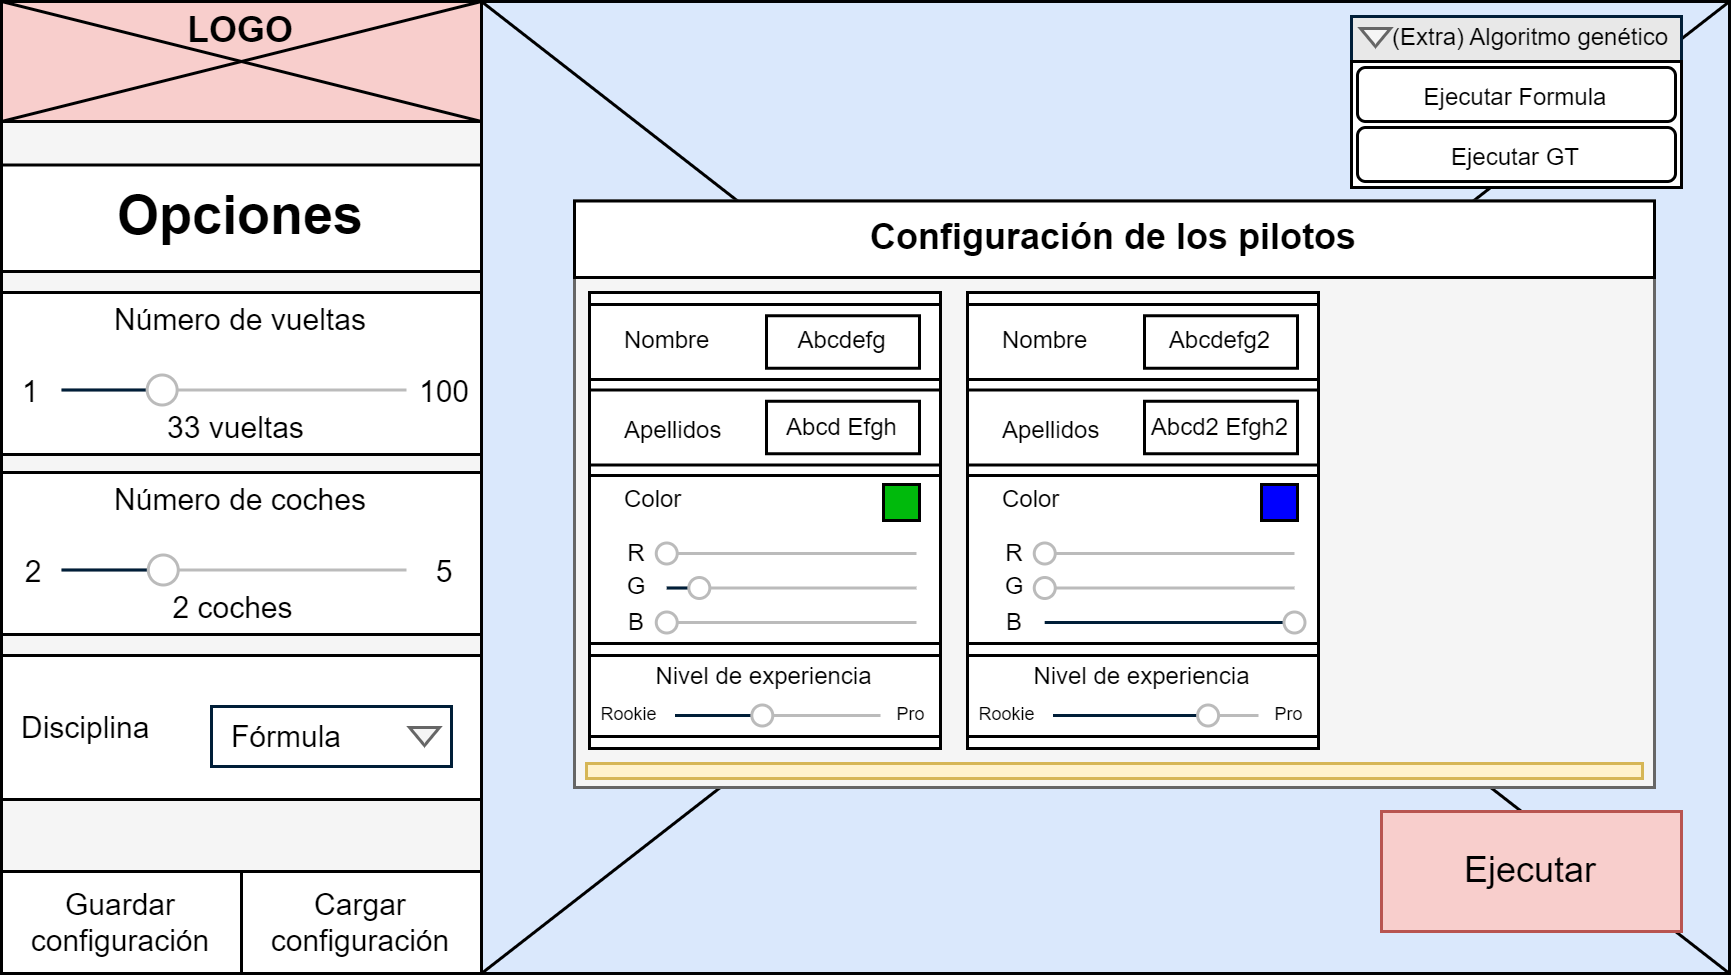
\includegraphics[width=\textwidth]{imagenes/pag1.png}
    \caption{Interfaz del configurador antes de la carrera.}
\end{figure}

\begin{figure}[H]
    \centering
    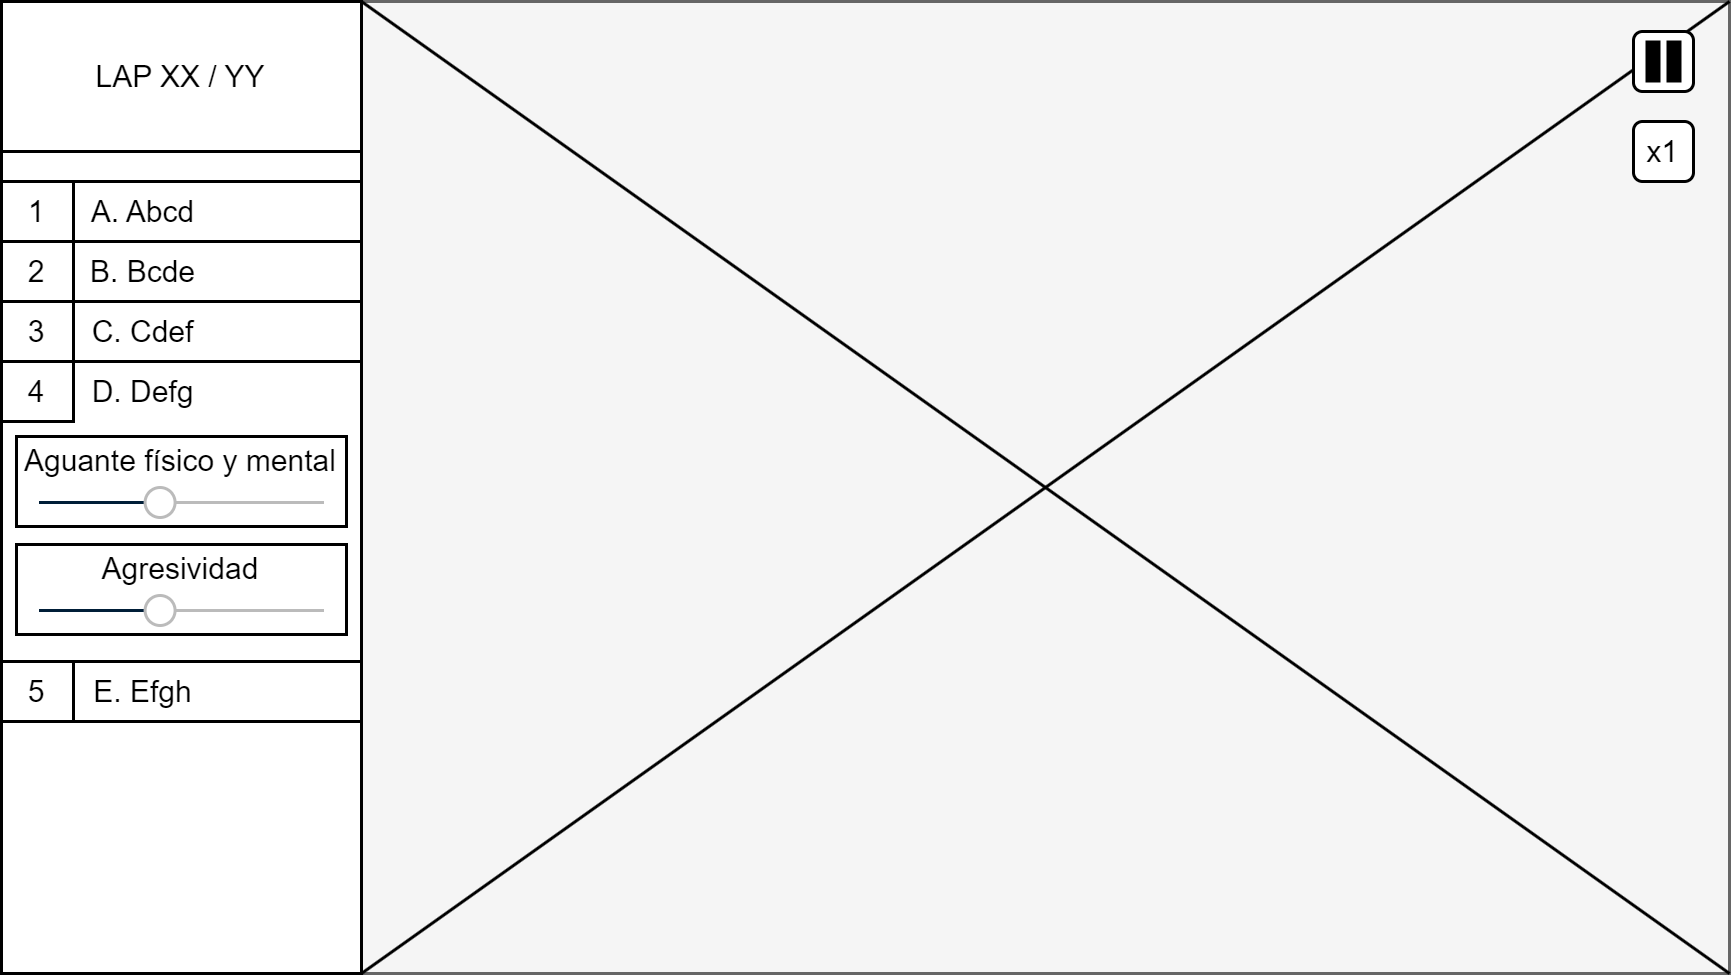
\includegraphics[width=\textwidth]{imagenes/pag2.png}
    \caption{Interfaz de las opciones durante la carrera.}
\end{figure}

\section{Diagrama de navegación}

La navegación por la interfaz de usuario en la aplicación es relativamente sencilla, al estar formada por dos pantallas: el configurador de simulación y la carrera en curso.

\bigskip
\newpage
El diagrama de navegación de la aplicación se encuentra a continuación:

% foto del diagrama de navegacion
\begin{figure}[H]
    \centering
    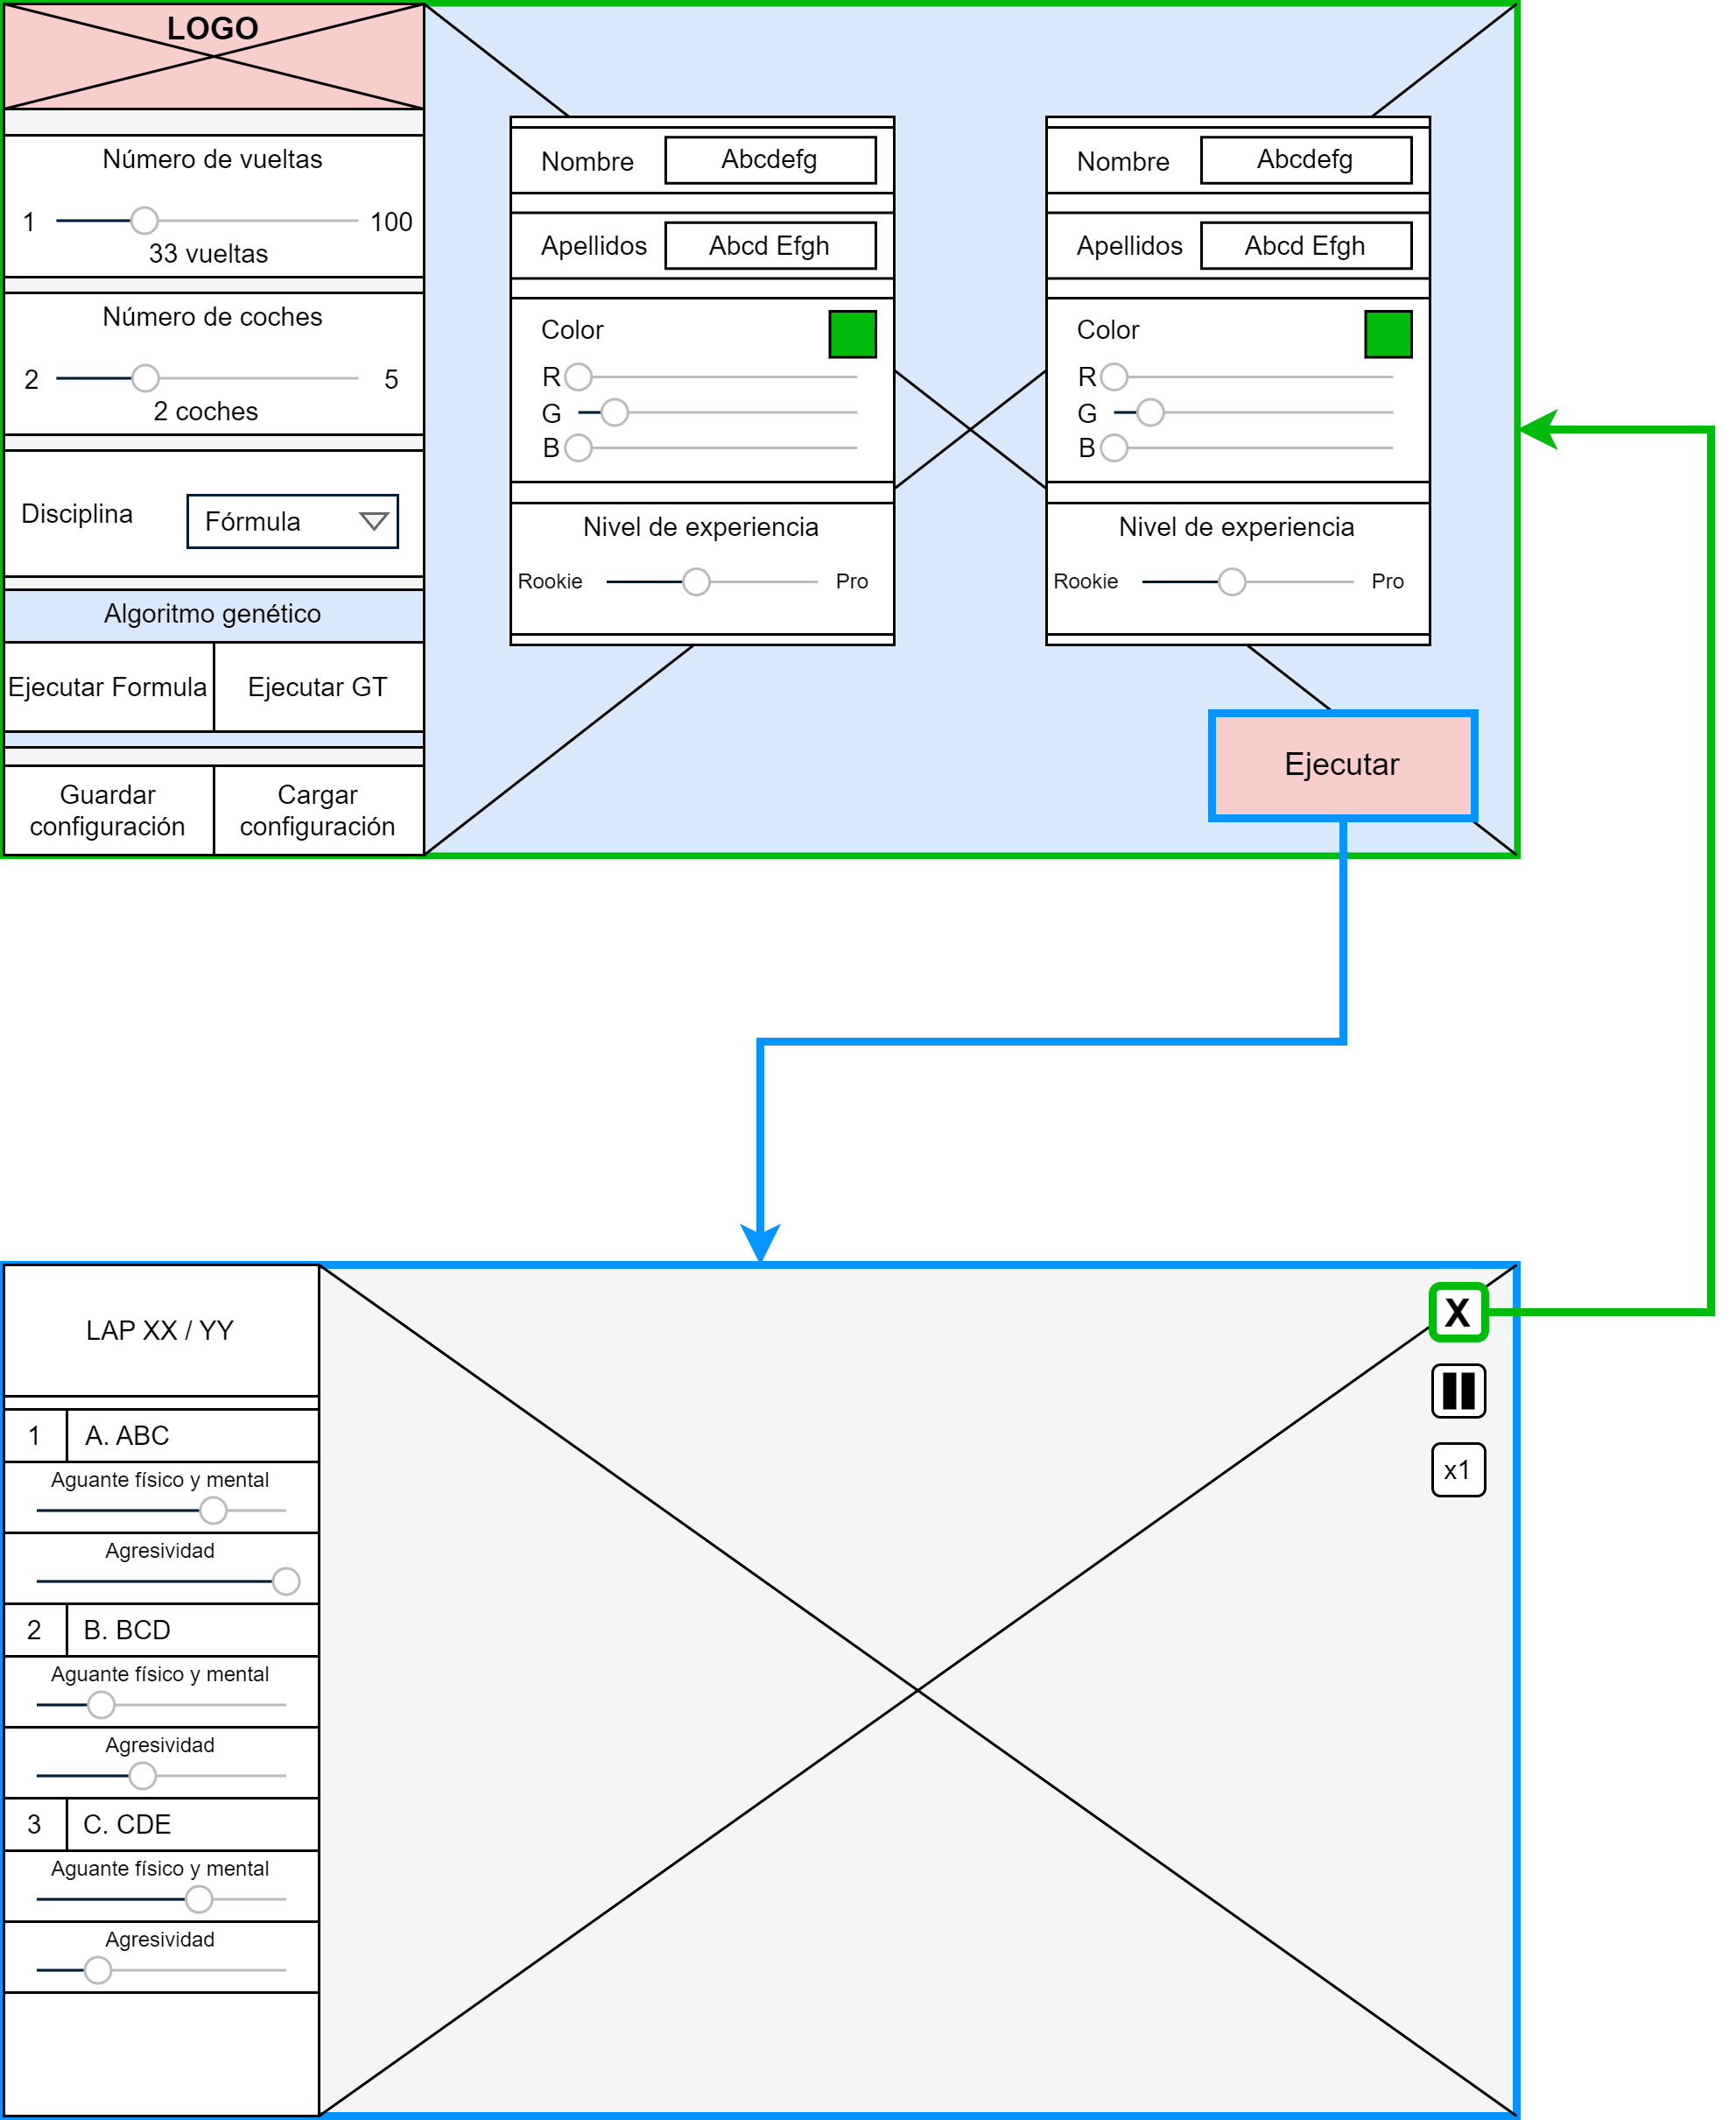
\includegraphics[width=0.9\textwidth]{imagenes/nav.png}
    \caption{Diagrama de navegación de la interfaz de usuario de la aplicación.}
 \end{figure}

Como se puede observar en el diagrama de navegación, al pulsar el botón de ejecutar aparecerá la nueva pantalla para ejecutar la simulación y dar comienzo a la carrera.

% Como se puede observar, la navegación por la aplicación es sencilla, al solo tener dos pantallas y un solo botón para ir a la siguiente. Si se pulsa sobre el botón de ejecutar en el configurador de la carrera, se procederá a cargar la simulación y dará comienzo la carrera.

% \chapter{Implementación}

Este capítulo tratará sobre las herramientas utilizadas para la implementación y planificación, así como los distintos algoritmos que se emplearán para realizar la simulación. Además, se detallará el diseño de los \textit{blueprints} y se describirán las reglas que seguirá el algoritmo de navegación.

\section{Herramientas utilizadas}

En el desarrollo del proyecto se utilizará \verb|git| para el control de versiones del proyecto.
%  y se almacenará en un repositorio de GitHub. 

\bigskip

Para el modelado, texturizado de los distintos objetos de la aplicación y el \textit{rigging} de los vehículos se utilizará Blender\cite{blender}.

\begin{figure}[H]
    \centering
    
\includegraphics[width=0.6\textwidth]{imagenes/blender-logo.png}
    \caption{Logotipo de Blender\cite{blender-logo}.}
    \label{fig:logoblender}
\end{figure}

Asimismo, para la creación y modificación de las texturas se utilizará GIMP\cite{gimp}.

\begin{figure}[H]
    \centering
    
\includegraphics[width=0.3\textwidth]{imagenes/gimp-logo.png}
    \caption{Logotipo de GIMP\cite{gimp}.}
    \label{fig:logogimp}
\end{figure}

\bigskip

% En cuanto a herramientas para la planificación, se hará uso de la herramienta \planApp para llevar un control de las Historias de Usuario que se realizan y pendientes en cada Sprint.
En lo que respecta a herramientas de planificación, se utilizará \planApp para llevar un control de las historias de usuario realizadas y pendientes en cada sprint. Además, se utilizará el \textit{power-up} ``Card Priority Badge'' de ``Kryl Solutions'' para poder anotar la prioridad de cada historia de usuario. Asimismo, se hará uso del \textit{power-up} ``Agile Tools by Corrello'' para poder tener estimaciones en las historias de usuario.

% foto de \planApp
% \begin{figure}[H]
%     \centering
%     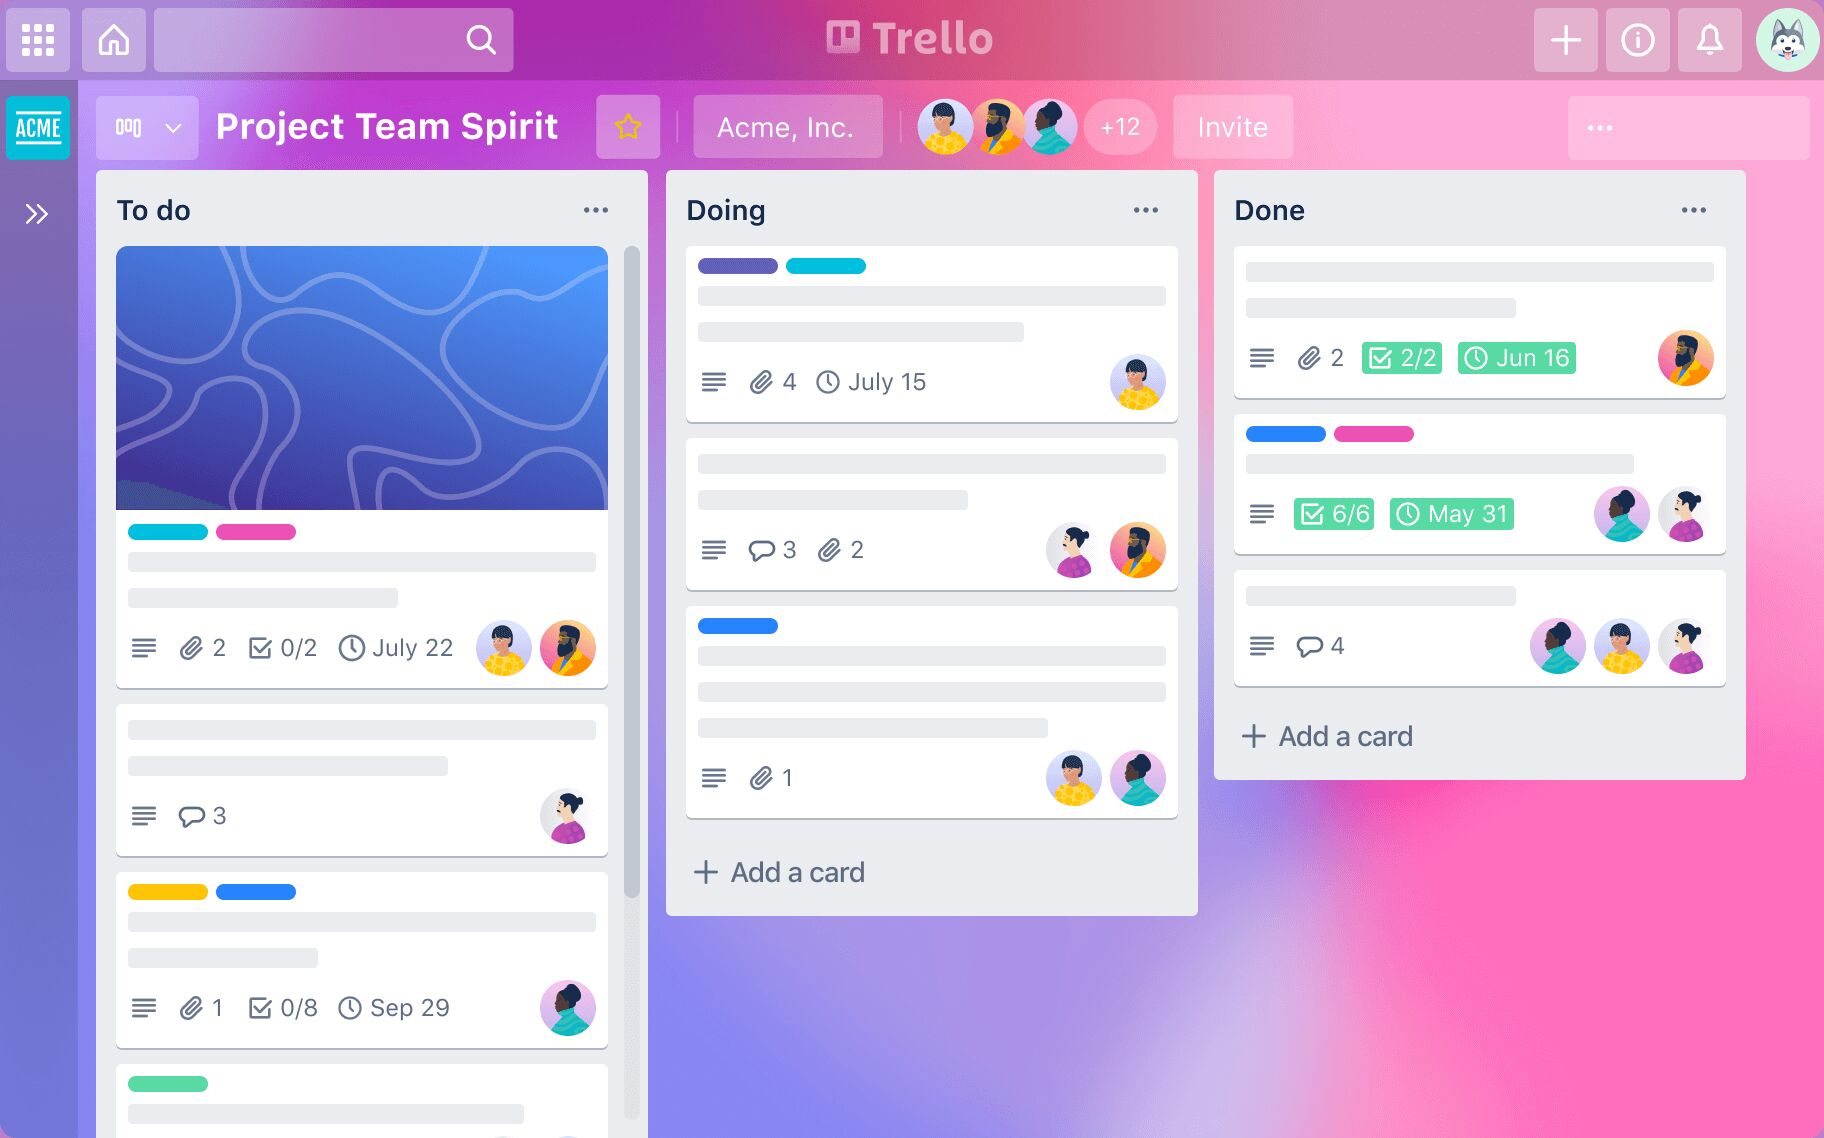
\includegraphics[width=\textwidth]{imagenes/converted/trello.jpg}
%     \caption{Tablero de ejemplo de Trello\cite{tablero-trello}.}
% \end{figure}
\begin{figure}[H]
    \centering
    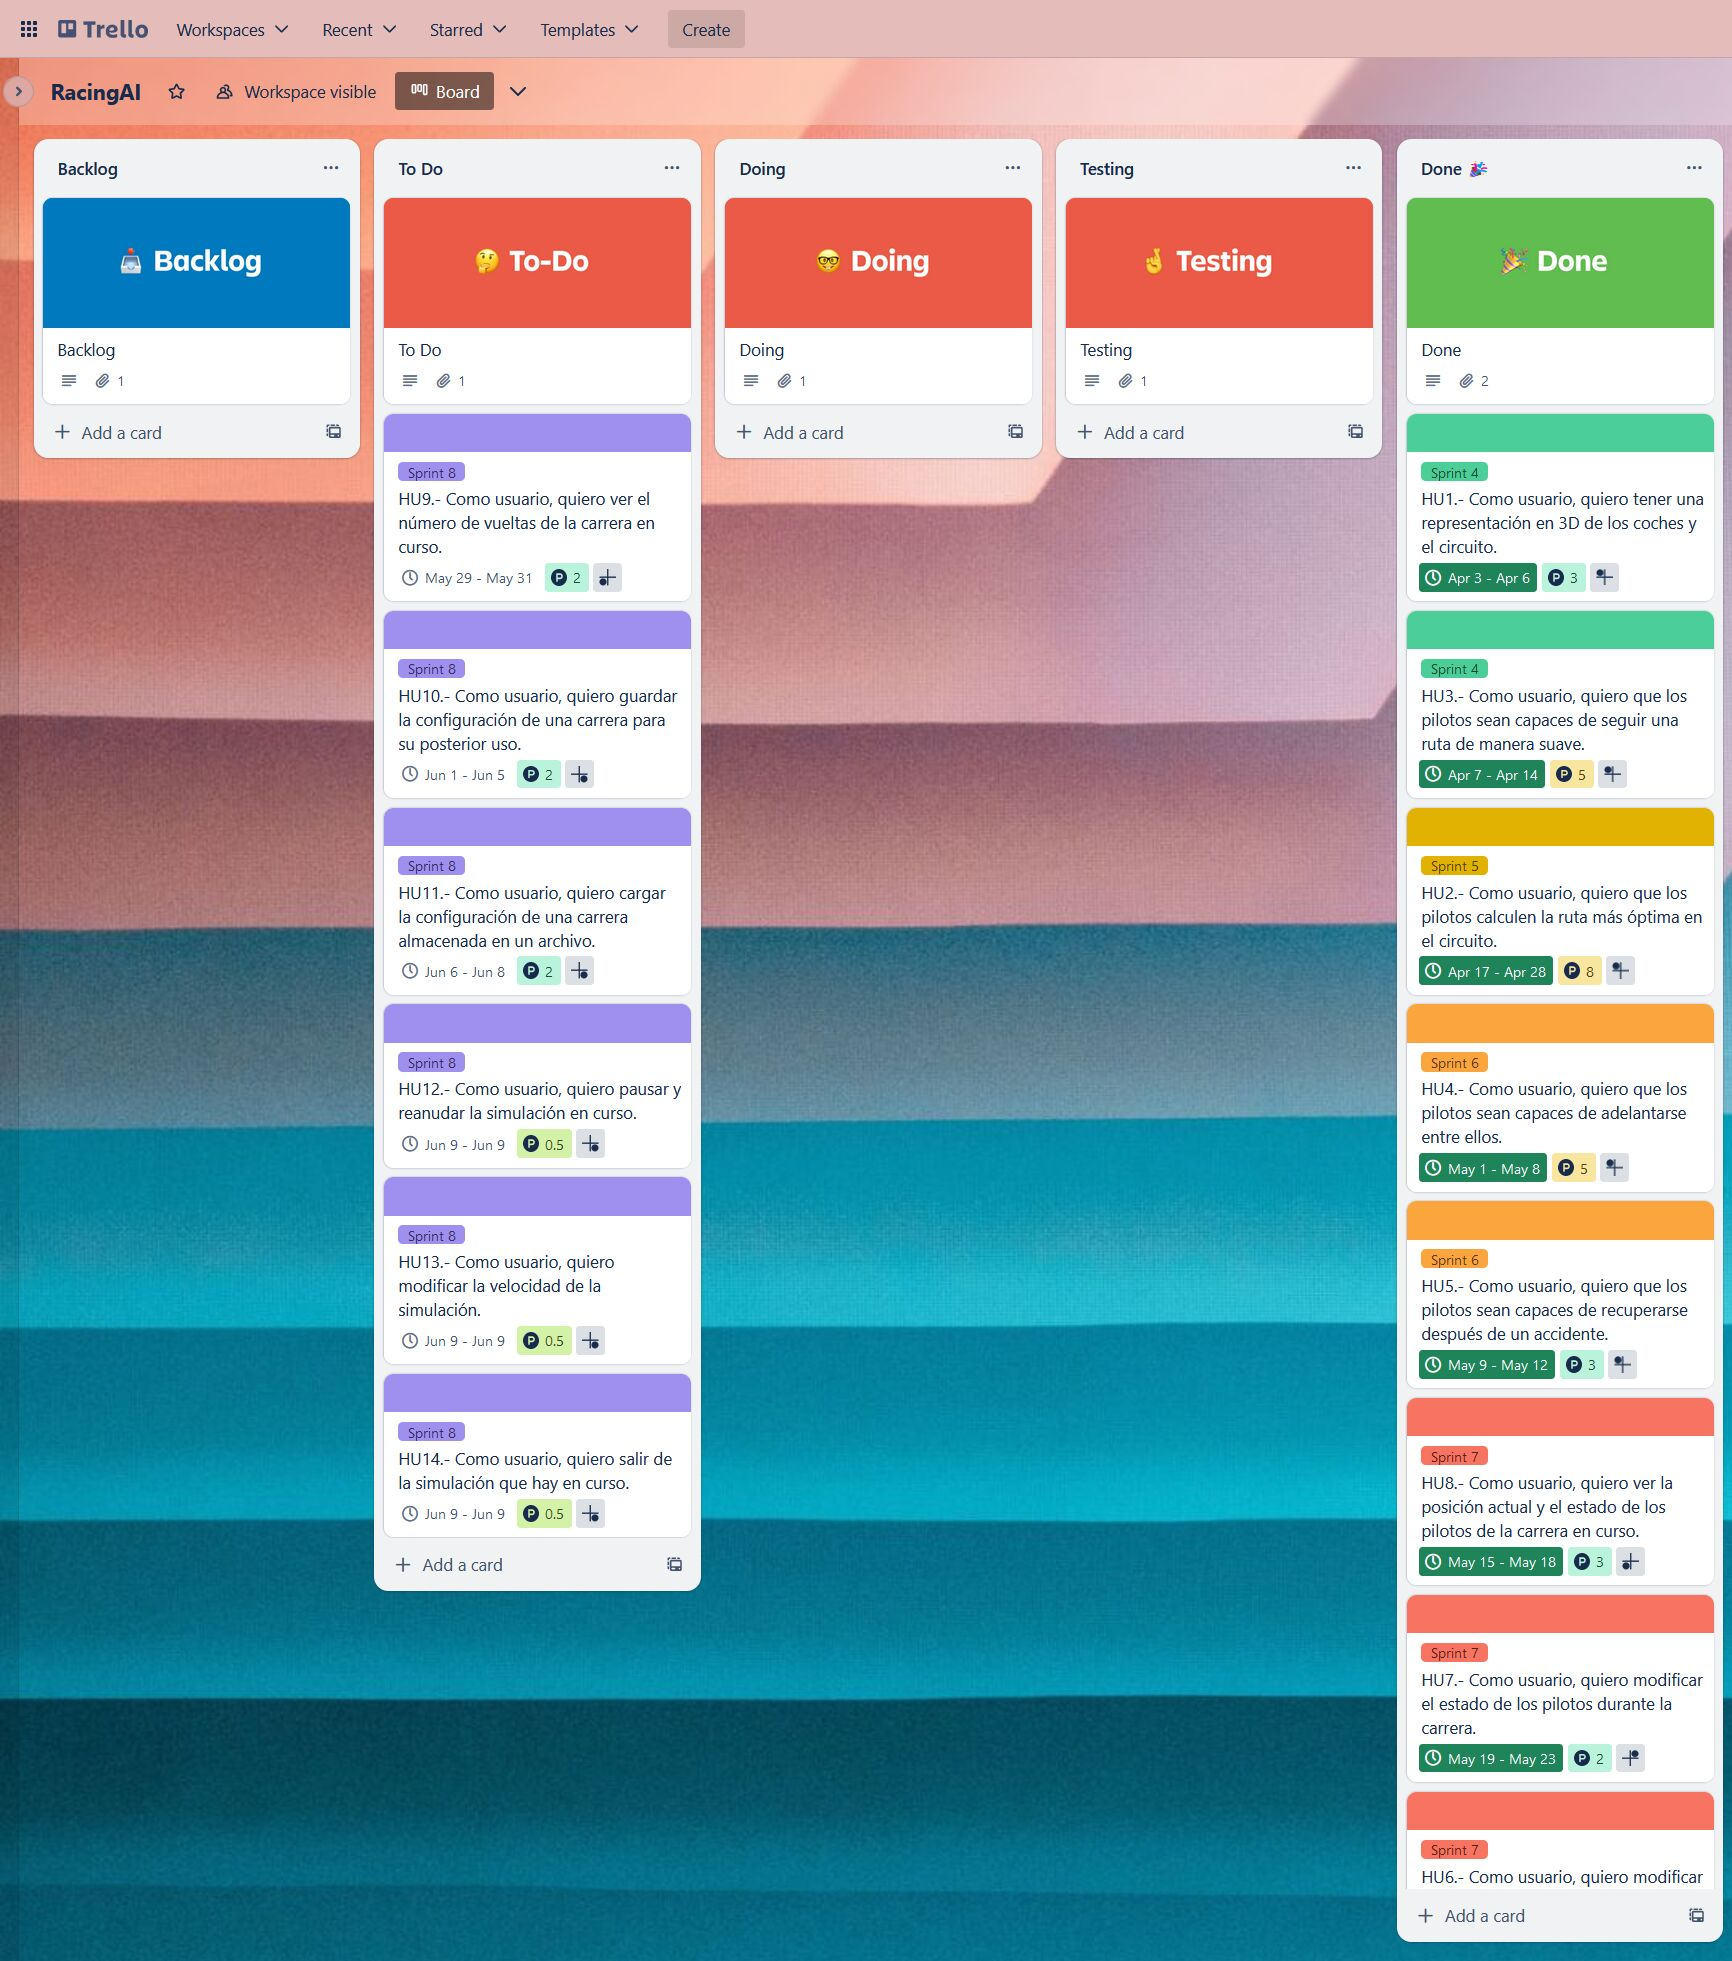
\includegraphics[width=\textwidth]{imagenes/converted/trello-mio.jpg}
    \caption{Tablero utilizado para el proyecto.}
\end{figure}

\newpage

\section{Glosario de términos de Unreal}
\label{sec:terminosunreal}
Esta sección es utilizada como una breve explicación de las palabras utilizadas referentes a Unreal Engine en este capítulo:

\begin{itemize}
    \item \textbf{Blueprint: }Forma visual de implementar lógica en el videojuego mediante el uso de nodos y aristas. Permiten programar sin necesidad de conocer la API en C++.
    \item \textbf{Evento (Event): }Acción o suceso que ocurre durante el juego y que puede desencadenar acciones o comportamiento. Los eventos pueden estar relacionados con el jugador, colisión entre objetos, etc.
    \item \textbf{Actor: }Es un objeto del mundo que puede tener presencia física, implementar comportamiento específico y ser creados en tiempo de ejecución. A grandes rasgos son una clase que pueden tener mallas de polígonos almacenadas.
    \item \textbf{Peón: }Tipo de actor que puede ser controlado directamente por el jugador. Por lo general, los peones representan personajes jugables en el juego.
    \item \textbf{Event ActorBeginOverlap: }Evento utilizado cuando un actor se superpone con otro actor. Puede ser utilizado para realizar acciones en caso de colisión.
    \item \textbf{Event ActorEndOverlap: }Evento que se activa cuando un actor deja de solaparse con otro. Puede ser utilizado para realizar acciones cuando se active el evento.
    \item \textbf{Event Tick: }Evento que ocurre cada fotograma del videojuego y puede desencadenar acciones. Se utiliza para acciones que necesitan actualizaciones continuas, como la animación, el control del volante y los pedales o el seguimiento de otros objetos.
    \item \textbf{Event Hit: }Evento que se activa cuando un objeto colisiona con otro objeto. Puede utilizarse para realizar acciones específicas cuando ocurre una colisión.
    \item \textbf{Line Trace: }Técnica utilizada para determinar si hay algún objeto colisionando con una línea recta que se traza desde un origen hasta un destino. A esta técnica se le llama también \textit{raycasting}.
\end{itemize}

\newpage

\section{Algoritmos utilizados}

Voy a dividir en subsecciones los diversos algoritmos que componen la simulación:

\subsection{Algoritmo para el giro del volante del coche}
\label{sec:pid-sec}

En el control del volante de los vehículos, correspondiente a HU3 y realizada en el sprint 4, se ha utilizado un controlador PID (\textit{Proportional, Integral} y \textit{Derivative}). Este controlador se utiliza para regular el error de un sistema de manera suave, evitando producir muchas desviaciones mediante el ajuste de tres constantes, una para cada componente del controlador. Cabe destacar que la variable a la que el sistema debe llegar se llama SP (\textit{Set Point}) y el valor actual del sistema se denomina PV (\textit{Process Variable}). 

\bigskip

Para que el controlador funcione bien, es necesario modificar sus tres constantes: 
% Proporcional, Integral y Derivativa. 

\begin{itemize}
    \item \textbf{Proporcional: }Actuará de manera proporcional al error actual, multiplicada por la constante asociada. Si solo se utiliza este componente, el sistema se pasará del SP, haciendo que tenga que volver a corregir, produciendo así demasiadas oscilaciones para llegar al SP. 

    \item \textbf{Integral: }Se encarga de derivar el error con respecto al tiempo, con el objetivo de anular errores residuales e incluso del propio sensor. Por normal general, seguirá pasándose del SP, ya que de esto se encarga la componente derivativa.

    \item \textbf{Derivativa: }Se utiliza para estimar como evolucionará la curva con el tiempo, basándose en su pendiente. Esta componente es la que se encarga de minimizar las oscilaciones, al reducir el efecto del actuador si se acerca demasiado rápido al SP.
\end{itemize}

\bigskip

% \lstinputlisting[language={[Visual]C++}, caption={Implementación en C++ del controlador PID}, label={lst:pidcpp}]{snippets/PID.cpp}

\begin{listing}[H]
    \caption{Implementación en C++ del controlador PID}
    \inputminted[fontsize=\scriptsize, linenos, bgcolor=LightGray, frame=lines, framesep=3mm, baselinestretch=1.2]{C++}{snippets/PID.cpp}
    \label{lst:pidcpp}
\end{listing}

El rango de valores que pueden tener las variables dependen del sistema al que se aplique. No obstante, todos los valores son números reales positivos, incluyendo el 0, que deshabilita la componente.

\bigskip

Cabe destacar que, en mi caso, el SP es el punto más cercano del coche a la ruta generada, y el error es la distancia del coche a dicho punto.

\begin{figure}[H]
    \centering
    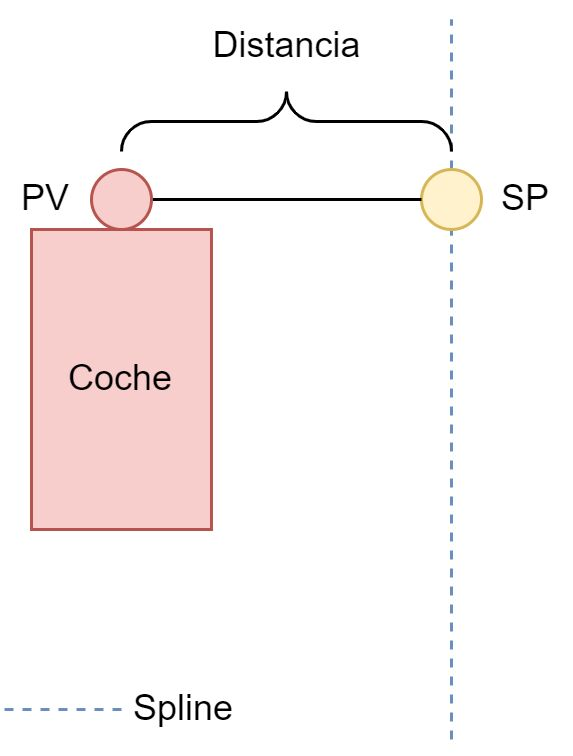
\includegraphics[width=0.4\textwidth]{imagenes/converted/errorPID.jpg}
    \caption{Esquema donde se indica el cálculo de la distancia para el PID.}
    \label{fig:errorpid}
    \end{figure}

La calibración del PID se realiza modificando las constantes asociadas a cada componente. Existen diversos métodos como el de Ziegler-Nichols \cite{10.1115/1.4019264}, que consiste en modificar solo la parte proporcional, dejando las demás a 0, hasta que el sistema comience a oscilar de manera estable, en ese momento se debe calcular la frecuencia a la que oscila y utilizando también el valor de la constante proporcional, se pueden obtener las demás mediante un cálculo matemático.

\bigskip

Dado que este método no me dio los resultados deseados, decidí implementar un algoritmo genético para obtener las constantes del controlador PID (implementación del controlador en Listing \ref{lst:pidcpp}). Consiste en lanzar un conjunto de coches con valores positivos aleatorios para las constantes del PID, con el objetivo de que intenten llegar a la meta con el menor error posible (por error se sigue entendiendo como la distancia del punto más cercano a la ruta con el coche, véase Figura \ref{fig:errorpid}). Aquellos con menos error, tienen más posibilidades de ser seleccionados para generaciones futuras. Una vez obtenido el error, se calcula su inversa y se obtiene la probabilidad de ser elegido mediante el nuevo valor entre la suma de todos. Esto dará como resultado unas probabilidades que al ser sumadas darán 1 (100\%). 

\bigskip
% imagen de ejemplo de selección de ruleta
\begin{figure}[H]
    \centering
    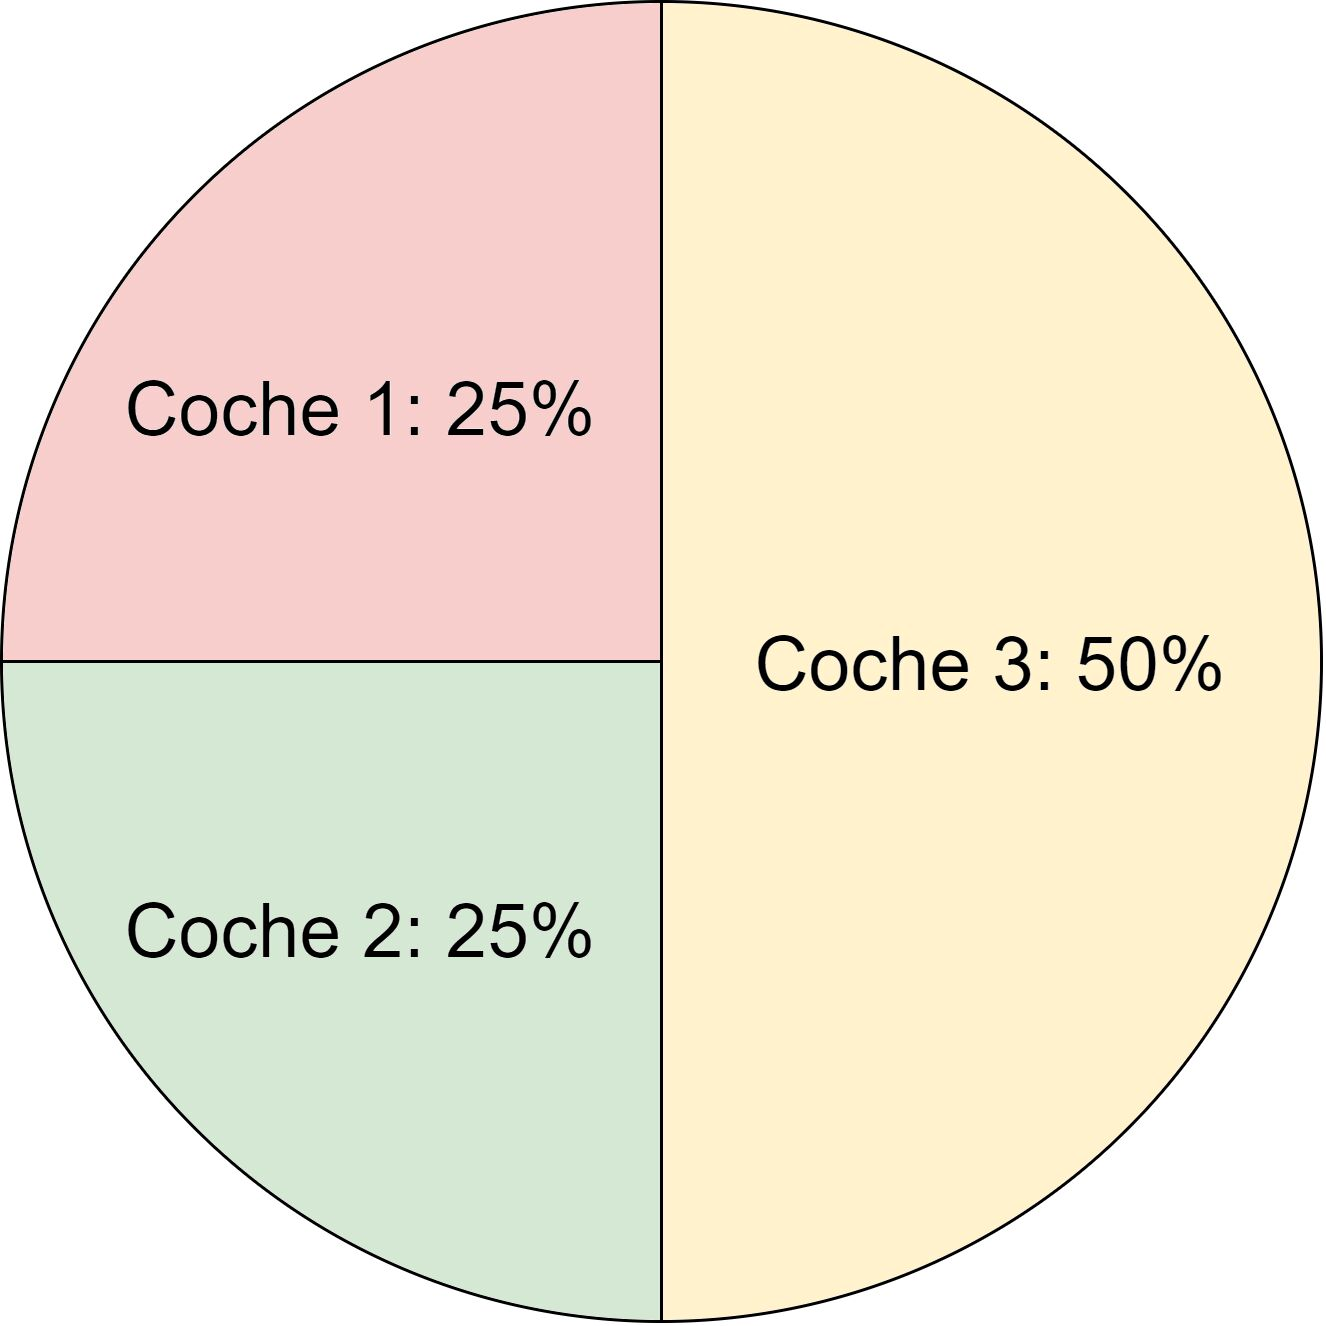
\includegraphics[width=0.4\textwidth]{imagenes/converted/ruleta.jpg}
    \caption{Ilustración de la selección por ruleta}
    \label{fig:ruleta}
\end{figure}

La selección se realiza lanzando una ruleta\cite{gaperformance}, cuyos sectores son divididos en función de la probabilidad calculada anteriormente. La ruleta se debe lanzar tantas veces como padres se desea tener. Una vez que se han elegido los coches que van a ser padres, se emparejan y se mezclan sus constantes para obtener dos hijos de cada pareja. Después, una de las tres constantes del PID en algunos de los hijos puede ser mutada, con una probabilidad del 33\%, con un valor aleatorio de rango [-0.1,0.1] que se le añade al valor existente. Finalmente se sustituyen los coches no elegidos para la siguiente generación por los hijos con las constantes mezcladas y mutadas, manteniendo a los padres, y se vuelve a ejecutar de nuevo el algoritmo.

\bigskip

Utilizando este algoritmo, obtuve unos valores que funcionaban bien para el circuito. No obstante, tras ejecutarlo varias veces, me he dado cuenta de que la constante integral siempre tiende a 0. Para solucionarlo, he decidido obligarle a que tenga un valor mínimo de 0,01.


\subsection{Algoritmo de navegación}

En cuanto al algoritmo de navegación, correspondiente a HU2, HU4 y HU5 e implementadas en los sprints 5 y 6, he utilizado A*\cite{4082128}, que es lanzado utilizando diversas reglas, y una componente reactiva. 

\bigskip

A* es utilizado para obtener rutas en un grafo. Para ello, hace uso de una función heurística para estimar la distancia restante al nodo destino. A diferencia de otros algoritmos, como el de Dijkstra, A* es más rápido, gracias a la heurística, ya que puede descartar nodos que están más alejados del destino.

\bigskip

El algoritmo se encarga de visitar todos los nodos vecinos, calculando el coste de llegar desde el origen y el coste para llegar al destino mediante la heurística, en caso de encontrar una ruta mejor de un nodo ya existente en la lista de abiertos, se elimina el anterior y se introduce el nuevo. Este proceso se repite hasta que se llega al destino o, en mi caso, llega a un límite de iteraciones.

\bigskip

En la figura \ref{fig:rutaastar} se pueden observar unos cubos rojos, que representan la ruta generada por el algoritmo de navegación desde el checkpoint (véase Figura \ref{fig:checkpointunreal}) de la derecha hasta el de la izquierda.

% PONER EJEMPLOS DE RUTAS GENERADAS
\begin{figure}[H]
    \centering
    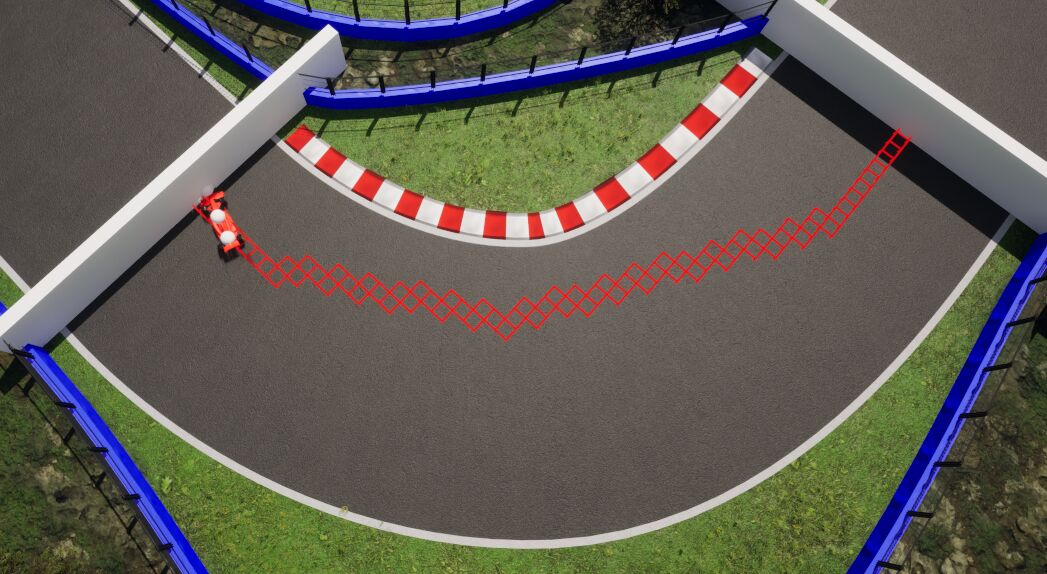
\includegraphics[width=0.7\textwidth]{imagenes/converted/rutaAStar.jpg}
    \caption{Ruta generada por un vehículo hasta el siguiente checkpoint.}
    \label{fig:rutaastar}
\end{figure}


Realicé una primera implementación del algoritmo A* utilizando \textit{blueprints}. Sin embargo, había casos en los que el programa se quedaba congelado unos segundos hasta encontrar la ruta. La solución fue implementar en \textit{blueprints} una cola con prioridad utilizando un \textit{Binary Heap}. Esta versión provocó una gran mejora en el tiempo de ejecución, pero para carreras con más de dos coches, el tiempo de ejecución seguía siendo demasiado grande, haciendo que el programa se quedase parado unas décimas de segundo.

\bigskip

Finalmente opté por implementarlo en C++, utilizando como cola con prioridad el \textit{Binary Heap} que implementan los arrays (TArray) de Unreal. Esta versión ha conseguido que no se produzcan más paradas en la simulación, de manera que ahora pueden correr más de dos coches al mismo tiempo.

\subsubsection{Heurística}

% Debido a que un nodo puede moverse en 8 direcciones distintas, incluyendo las diagonales, es necesario utilizar una heurística acorde. Por tanto, he decidido utilizar la distancia Chebyshev\cite{enwiki:1149051498}, cuyos movimientos diagonales tienen el mismo coste que los demás. 

% \bigskip

% La configuración de los nodos prohíbe utilizar una heurística como la distancia Manhattan, ya que sobrestimaría la distancia al destino, haciendo que no sea correcto.

La heurística elegida ha sido la distancia Manhattan, ya que el rango de movimiento en la malla es solamente vertical y horizontal.

% foto diagrama de la distancia manhattan
\begin{figure}[H]
    \centering
    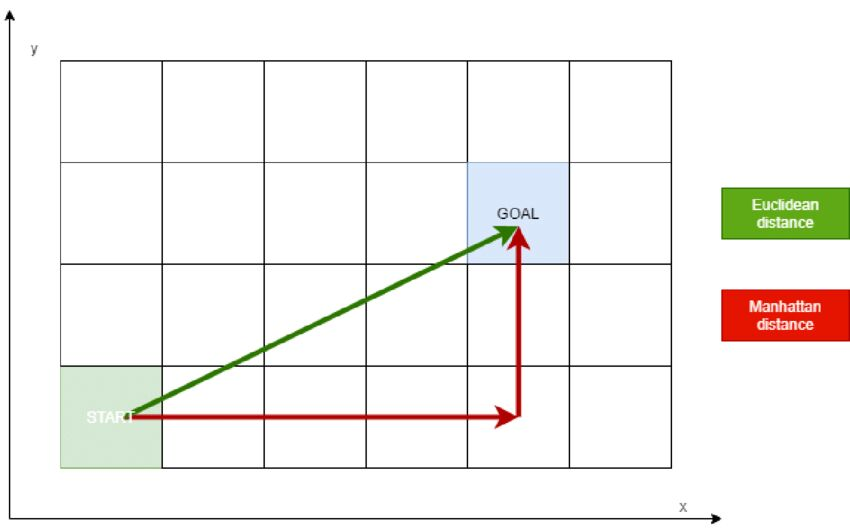
\includegraphics[width=0.7\textwidth]{imagenes/converted/Euclidean-and-Manhattan-distance-comparison-3235-Optimizations-The-first-optimization.jpg}
    \caption{Esquema del funcionamiento de la distancia Manhattan\cite{gameai}.}
    \label{fig:manhattan}
\end{figure}


\subsection{Generación de la malla de navegación}
Para que A* funcione, es necesario discretizar el espacio y crear una estructura de datos que permita incluir todos los posibles estados para que los pilotos puedan tomar decisiones.

\bigskip

% En cada subsección se hablará de cada componente que forma la malla de navegación:
A continuación se da una explicación de cada uno de los elementos que forman la malla de navegación:

\begin{itemize}
    \item \textbf{Nodo: }Para implementarlo, he creado un actor (véase sección \ref{sec:terminosunreal}) que representa un nodo. Además, posee las variables necesarias para saber si se encuentra un vehículo dentro de él, si es un delimitador de límites de pista, si es un checkpoint o si es una guía de ruta óptima. De esta forma se puede tener un control muy alto sobre los pesos de cada estado. Además, cada nodo almacena una referencia a sus nodos adyacentes, para que puedan ser utilizados por el algoritmo A*.
    
    \bigskip
    
    La actualización de un nodo de un estado a otro se realiza mediante el evento \textit{ActorBeginOverlap} y \textit{ActorEndOverlap} (véase sección \ref{sec:terminosunreal}). Así se puede actualizar el mapa en tiempo real.
    
    \bigskip
    
    Cabe destacar que los nodos con estado checkpoint y delimitador no pueden ser cambiados de estado; es decir, el delimitador de pista siempre estará ocupado, dándole un coste mayor. Mientras que el checkpoint siempre estará libre, dándole un coste menor. Los checkpoints nunca reciben colisión para optimizar la velocidad del algoritmo A*, ya que si se tienen en cuenta puede llegar a tardar demasiado en encontrar la ruta.
    
    \bigskip
    
    El estado ruta óptima sirve para darle una ayuda a los coches, ya que si no se utilizase escogería rutas más rígidas. Este estado no prohíbe a los coches la posibilidad de elegir otra ruta para adelantar o volver a pista, solo es una guía.
    
    \bigskip
    
    La construcción del delimitador y de la ruta óptima la he realizado utilizando actores distintos, de manera que se activen los eventos anteriormente mencionados para que se ajusten.

    \bigskip

    En la figura \ref{fig:nodo} se puede ver la representación de un nodo en el mapa. Asimismo, se puede observar como los nodos tienen cierta altura en el eje Z (mundo Z-Up), aun siendo utilizado para calcular una ruta en dos dimensiones. Esto se debe a que los vehículos deben solaparlos (con los eventos mencionados anteriormente) para poder actualizar cada nodo con el estado correcto.

    \begin{figure}[H]
        \centering
        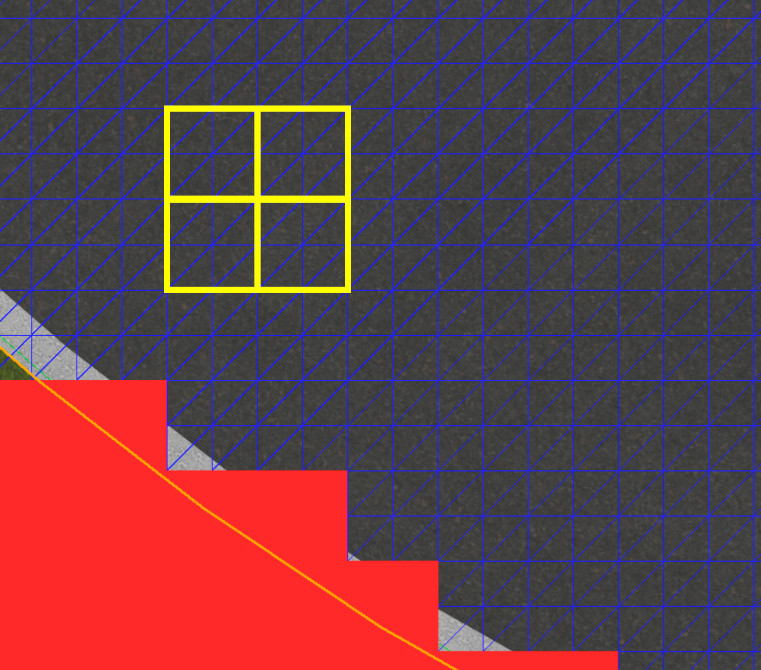
\includegraphics[width=0.5\textwidth]{imagenes/converted/nodesCropped.jpg}
        \caption{Visualización de varios nodos en el mapa. Cada nodo es representado por cuatro cuadrados. Se han resaltado en color amarillo cuatro nodos.}
        \label{fig:nodo}
    \end{figure}

    \item \textbf{Malla (conjunto de nodos): }Para realizar la malla de navegación he utilizado un actor encargado de generar los nodos mencionados anteriormente en una malla de \gridSize. Como he dicho antes, estos valores pueden ser modificados, incluido el offset de donde comienza a generar nodos.
    
    \bigskip
    
    Este actor incluye los métodos necesarios para poder direccionar un nodo de la malla como una matriz (con filas y columnas), poder obtener su posición en coordenadas del mundo y poder convertir de coordenadas del mundo a coordenadas de matriz.

    % foto de la malla recreada en unreal
    \begin{figure}[H]
        \centering
        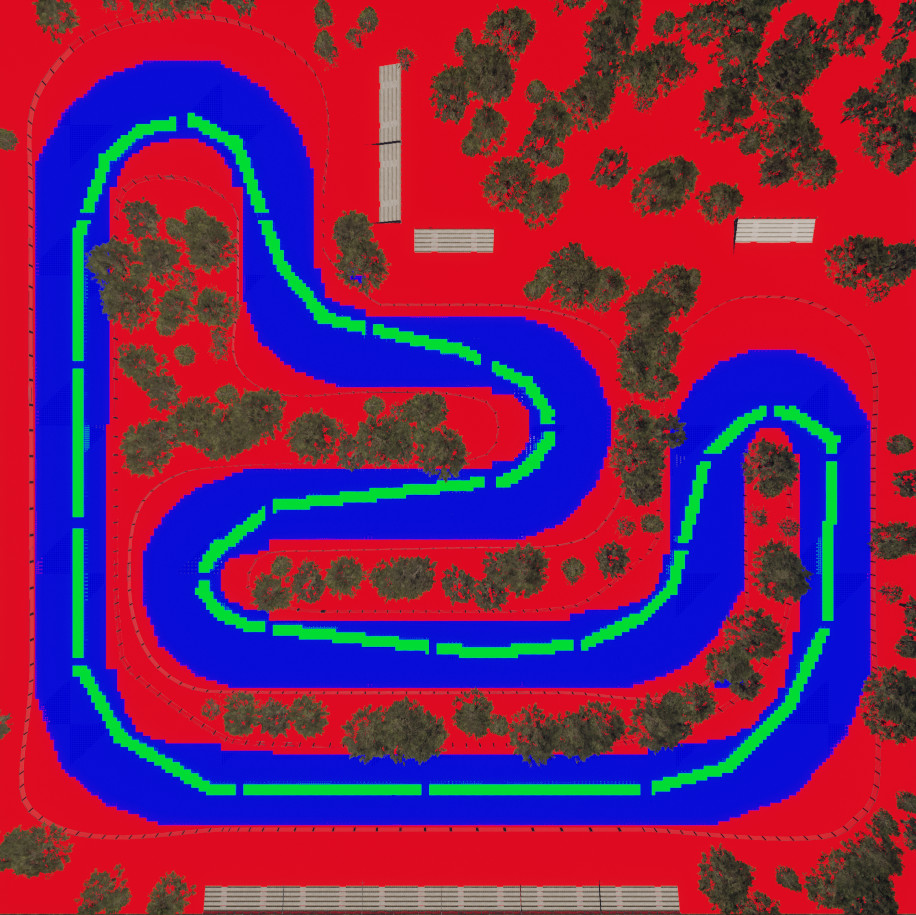
\includegraphics[width=0.6\textwidth]{imagenes/converted/malla.jpg}
        \caption{Malla de navegación generada sobre el circuito. Los puntos rojos son muros, los verdes indicadores de ruta óptima y los azules el resto de la pista utilizable.}
        \label{fig:mallanav}
    \end{figure}
\end{itemize}


\subsection{Cálculo de la ruta por los vehículos}

Con todo lo anterior implementado el coche es capaz de obtener una ruta por el circuito. No obstante, sigue siendo demasiado costoso obtener una ruta demasiado larga, para luego tener que desecharla por un adelantamiento o un choque. Es por eso que he dividido el circuito en varios checkpoints de tamaño relativamente reducido, con el objetivo de que el cálculo de rutas sea más rápido.


% foto de los checkpoints
\begin{figure}[H]
    \centering
    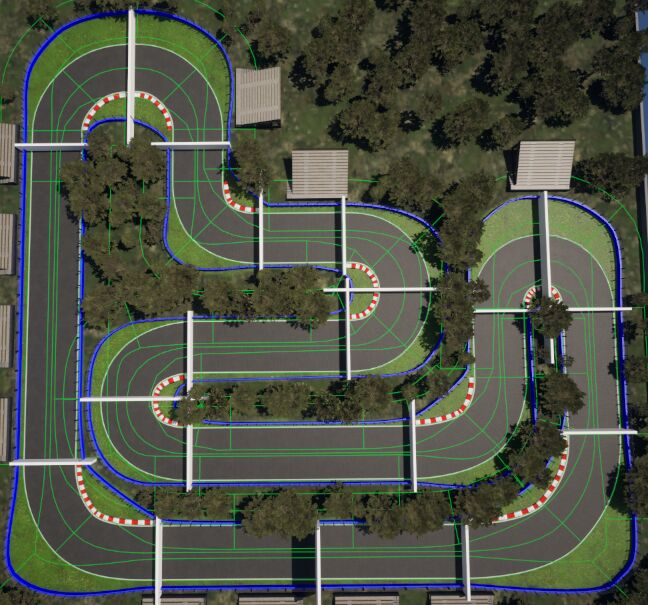
\includegraphics[width=0.6\textwidth]{imagenes/converted/checkpoints.jpg}
    \caption{Checkpoints utilizados a lo largo del circuito. Los checkpoints son las líneas de color blanco. Además, hay otra en la línea de meta.}
    \label{fig:checkpointunreal}
\end{figure}

Cuando la parte delantera del vehículo se solapa con un checkpoint, calcula la ruta utilizando A* hasta el siguiente. La llamada al algoritmo devuelve un vector de puntos en coordenadas del mundo. El vehículo se encarga de filtrar los puntos generados para que solo haya uno en cada checkpoint, ya que en otro caso puede generar problemas en el seguimiento de la ruta.

\bigskip

Con los puntos filtrados, el coche construye un spline y pinta los puntos en el suelo. Este spline será seguido gracias al controlador PID (Listing \ref{lst:pidcpp}) mencionado anteriormente. Cabe destacar que al ser la ruta discreta y el vehículo una componente física del mundo, el vehículo no siempre conseguirá seguirla siempre, pero le servirá como ``guía'' a la hora de tener que hacer giros y adelantamientos.

\newpage

\subsection{Lógica de adelantamiento de los vehículos}


Dado que el algoritmo A* funciona principalmente para mundos estáticos, es necesario actualizar la ruta si se realiza un cambio de posición en los vehículos. En este caso, para adelantar al contrincante.

\bigskip

La regla que sigue el vehículo es si se encuentra a una distancia del vehículo de adelante y tiene la suficiente diferencia de velocidad, ejecuta el algoritmo de navegación y espera unos pocos segundos para volverlo a ejecutar. Esta implementación me ha dado unos resultados razonables en tiempo y habilidad en los pilotos.

\bigskip

En la figura \ref{fig:overtake} se puede ver como se han dado las condiciones necesarias en el coche verde y ha recalculado la ruta para intentar adelantar al coche rojo.

% quizas poner foto, pero creo que va a ser complicado
\begin{figure}[H]
    \centering
    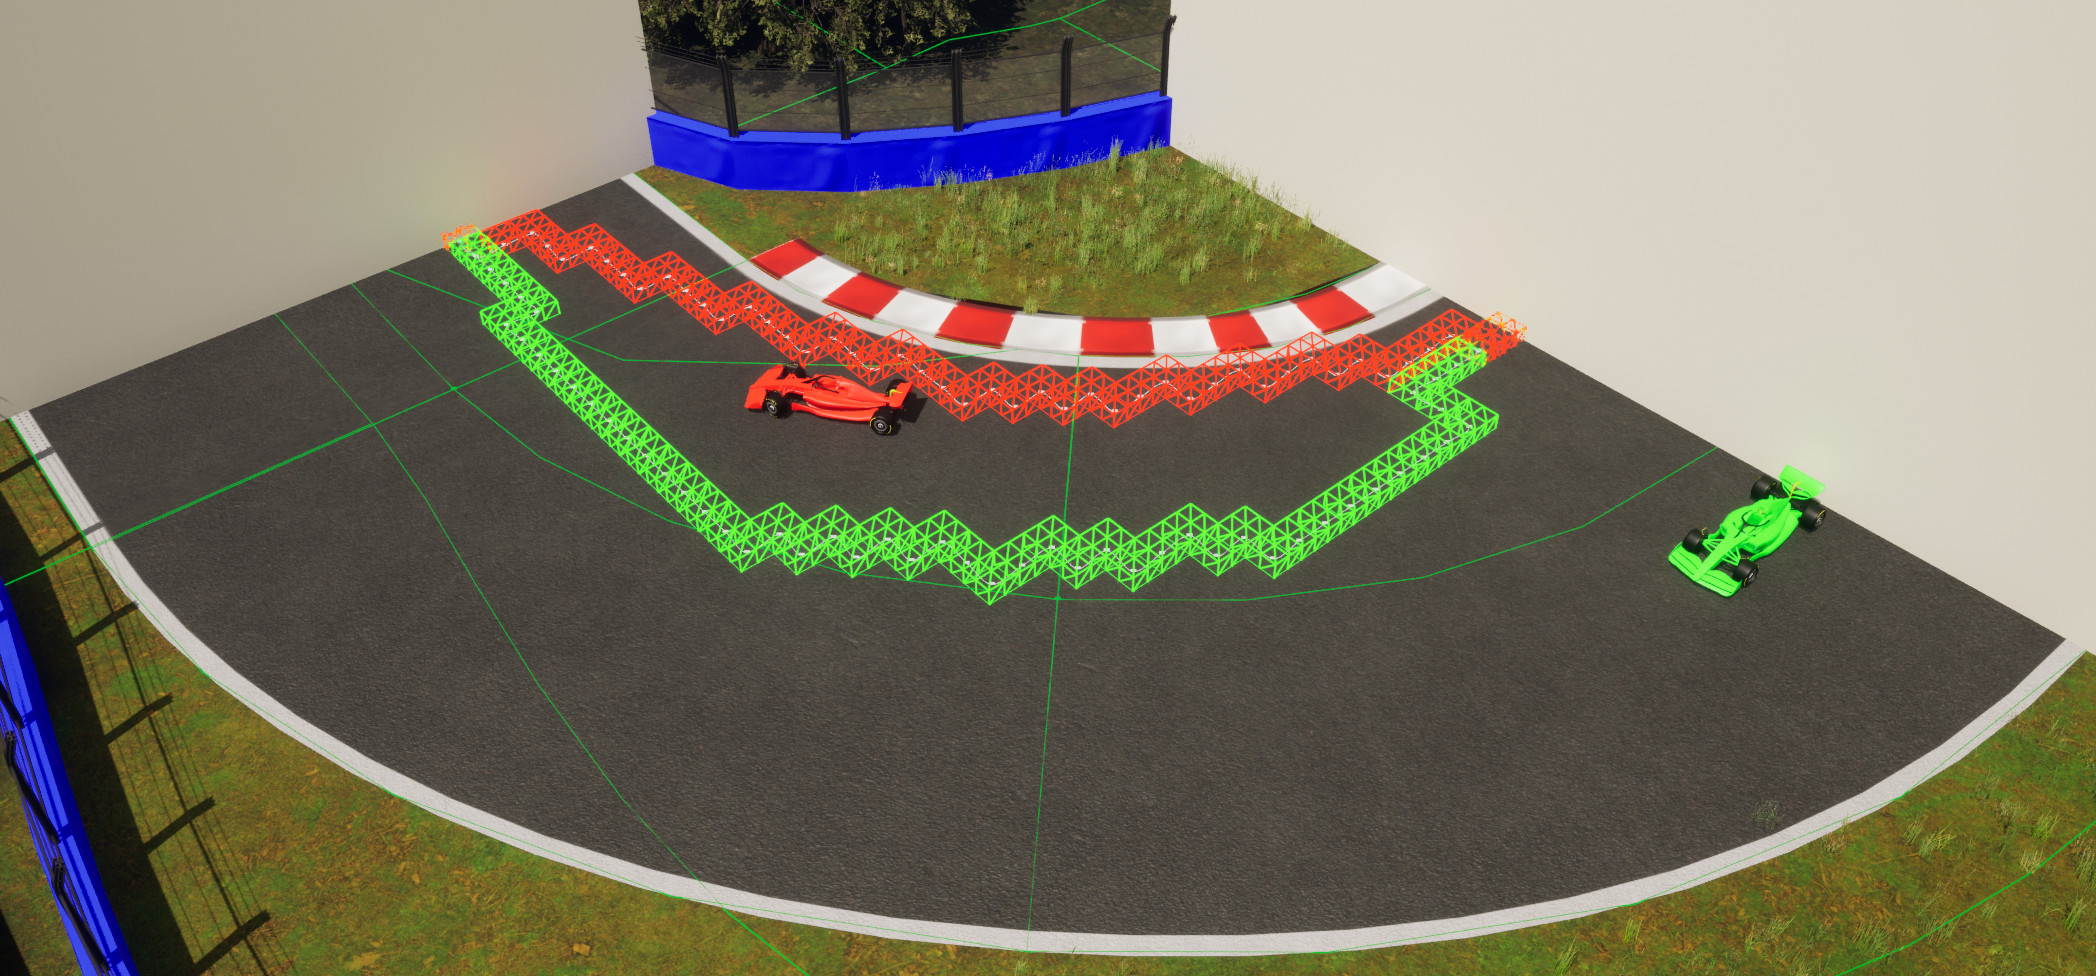
\includegraphics[width=0.6\textwidth]{imagenes/converted/overtake.jpg}
    \caption{Cálculo de la ruta del coche verde para intentar adelantar al otro piloto.}
    \label{fig:overtake}
\end{figure}

\subsection{Recuperación después de un accidente}

Si un coche se sale de pista primero se esperan unos segundos para comprobar que de verdad no se puede mover. Cuando se ha comprobado, se recorre un cierto tiempo marcha atrás con las ruedas rectas. Finalmente, ejecuta el A* para calcular una ruta de escapatoria y recorre lento dicha ruta por un breve instante de tiempo, hasta que finalmente recupera la velocidad que tenía.

\subsection{Recuperación después del vuelco}

Puede darse el remoto caso de que un vehículo vuelque y no sea capaz de darse la vuelta. En este caso he decidido implementar una regla que comprueba si la rotación del coche es mayor de 90 grados en ambos sentidos, pone el coche de nuevo sobre sus cuatro ruedas.

% HERE: PONER FOTO DEL CODIGO PARA DAR LA VUELTA

\subsection{Frenada anticipativa para evitar colisión}
\label{sec:frenada}

Dado que mucha de las veces los vehículos calculan rutas casi idénticas, puede darse el caso de que el vehículo de atrás provoque un accidente con el de delante. Es por eso que es necesario implementar una forma para que los vehículos de detrás frenen.

\bigskip

Para ello, he hecho uso de los \textit{Line Trace} (véase sección \ref{sec:terminosunreal}) para poder trazar un rayo hacia adelante y comprobar si hay un coche cerca. En la figura \ref{fig:esqlinetrace} aparece un boceto de como funciona:

\begin{figure}[H]
    \centering
    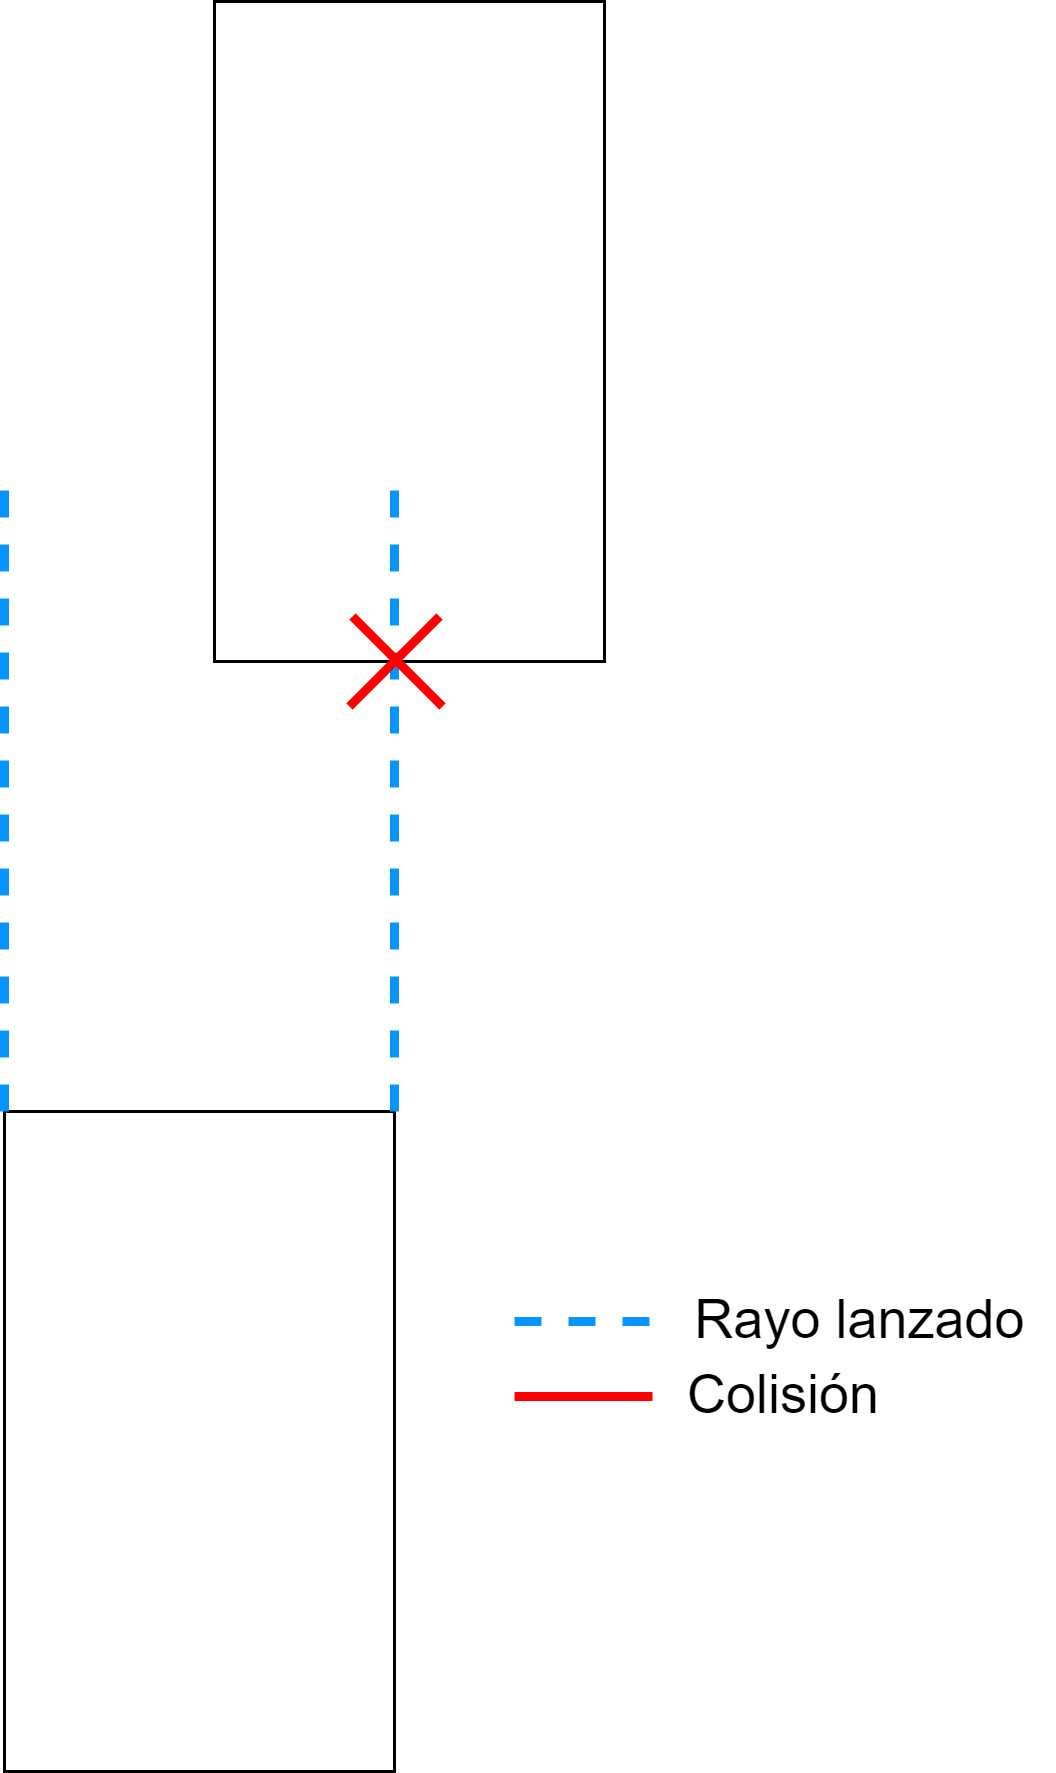
\includegraphics[width=0.3\textwidth]{imagenes/converted/raycast.jpg}
    \caption{Esquema del trazado de rayos.}
    \label{fig:esqlinetrace}
\end{figure}

\bigskip

Además, para evitar colisiones entre vehículos, he calculado la distancia de los rayos en función de la velocidad, de forma que a mayor velocidad, mayor distancia del rayo. También he tenido en cuenta el nivel de agresividad y si el vehículo se encuentra al final de una recta, ya que existe el riesgo de colisionar con el vehículo de delante que frena antes y puede tener menor velocidad al no estar agresivo.

\bigskip

Los resultados obtenidos para niveles de agresividad altos son buenos, ya que en la mayoría de las ocasiones logra frenar a tiempo. Sin embargo, en algunas situaciones, se produce una colisión, lo cual simula el riesgo asumido por un piloto agresivo.

% HERE: PONER FOTO DEL CODIGO PARA FRENAR

\subsection{Rebufo de los vehículos}

Para dar algo más de realismo a la simulación, he implementado un sistema de rebufo básico. La implementación es similar a la de la sección \ref{sec:frenada}, utilizando \textit{Line Trace} para detectar si algún vehículo está delante, en caso afirmativo, se le aplica un impulso adicional al vehículo, de manera que tenga más aceleración de la normal.

\subsection{Control de acelerador y freno}

El control del acelerador y del freno en condiciones normales de carrera se implementa incluyendo en cada checkpoint (Figura \ref{fig:checkpointunreal}) la velocidad recomendada a la que debe ir el coche. El coche calcula la distancia a la que se encuentra del siguiente checkpoint y la distancia de frenado necesaria basándose en la velocidad y la desaceleración por el frenado (también se incluye la componente de agresividad).

\bigskip

Cabe destacar que esta velocidad es modificada por el estado del piloto, explicado en la sección \ref{sec:mod-estado-piloto}.

% HERE: AÑADIR FOTO DEL CODIGO QUE AUMENTA EL IMPULSO

\subsection{Algoritmo para las posiciones de los pilotos}

En lo que se refiere al cálculo de las posiciones de cada piloto, correspondientes a HU7 y HU8 e implementadas en el sprint 7, he utilizado una estructura de datos algo más compleja. Los vehículos almacenan la vuelta en la que están y el checkpoint; es decir, el sector del circuito en el que se encuentran. Con la información anterior, he creado un array asociativo que almacene como clave la vuelta y como valor otro array asociativo, que a su vez tiene como clave el checkpoint y como valor un array con todos los vehículos que se encuentran en ese estado. Para mostrarlo, solo hace falta iterar primero por aquellas claves mayores, ya que son los que más vueltas y más lejos del circuito están.

\begin{table}[H]
    \caption{Representación de la estructura de datos que almacena las posiciones de los pilotos durante la carrera.}
    \footnotesize
    \centering
    \begin{tblr}{
        cells = {c},
        row{1} = {Silver},
        cell{1}{2} = {c=2}{},
        cell{2}{1} = {r=4}{},
        cell{2}{2} = {Alto},
        cell{2}{3} = {Alto},
        cell{7}{1} = {r=2}{},
        cell{7}{2} = {Alto},
        cell{7}{3} = {Alto},
        vlines,
        hline{1-2,6-7,9} = {-}{},
        hline{3-5,8} = {2-3}{},
            }
        \textbf{Clave (vuelta actual)} & \textbf{Valor }                    &                \\
        0                              & \textbf{Clave (checkpoint actual)} & \textbf{Valor} \\
                                       & 0                                  & {[}c1]         \\
                                       & ...                                &                \\
                                       & i                                  & {[}c2, c3]     \\
        ...                            & ...                                & ...            \\
        i                              & \textbf{Clave (checkpoint actual)} & \textbf{Valor} \\
                                       & 3                                  & {[}c4]
    \end{tblr}
    \normalsize
    \label{fig:tablapos}
\end{table}

% Para saber cuando lanzar la actualización de la lista de posiciones, cada coche calcula si el que está por delante de él sigue así, en caso contrario lanza el evento de actualización.

Para saber cuando lanzar la actualización de la lista de posiciones, cada coche comprueba si ha conseguido adelantar al coche que estaba inmediatamente delante de él, en caso afirmativo lanza el evento de actualización.


\subsection{Contador de vueltas}

En cuanto a la actualización del contador de vueltas, correspondiente a HU9 y realizado en el sprint 8, he hecho que todos los coches cuando acaben una vuelta intenten actualizarlo, en caso de que la vuelta actual sea mayor o igual, no se actualiza. De esta forma, es más fácil llevar un control más preciso de las vueltas.

\subsection{Resultados de la simulación}

Cuando el último coche cruza la línea de meta, aparece una tabla con los resultados de la carrera. La implementación de esta funcionalidad la he hecho comenzando con un array vacío para almacenar los vehículos a medida que llegan a la meta. Al llegar el último vehículo, se genera la tabla con las posiciones correspondientes al array. En la figura \ref{fig:resultados-sim} se encuentra el boceto de la interfaz.


\subsection{Importación y exportación de la configuración}

En la importación y exportación de la configuración, correspondiente a HU10 y HU11 y realizadas en el sprint 8, he deseado que el usuario sea capaz de elegir la ubicación del archivo y la ruta de guardado, respectivamente. 

\bigskip

Unreal implementa los métodos ``OpenFileDialog'' y ``SaveFileDialog'' para abrir el cuadro de diálogo de Windows, pero solo están disponibles en las versiones de desarrollo, produciendo un error fatal cuando se utiliza en la aplicación compilada para ser distribuida, ya que el módulo con los métodos no se incluye. Para evitar que ocurra el error, he incluido todo el código de ambos métodos en una clase de C++ denominada ``FileDialogHandler'', con los métodos ``abrirArchivo'' y ``guardarArchivo'', de forma que se pueda utilizar en versiones de producción de la aplicación.

\bigskip

El formato del archivo generado es un JSON en el que se encuentran los atributos como: el número de vueltas, y cada uno de los coches con sus capacidades.

\bigskip

Para poder cargar y guardar los archivos, he utilizado el plugin ``JSON Blueprint Utilities'' de Epic Games, que viene por defecto en Unreal Engine 5, pero deshabilitado.

\subsection{Cambio entre distintas cámaras}

La funcionalidad de cambiar la cámara, correspondiente a HU16 y desarrollada en el sprint 9, permite visualizar la carrera entre tres tipos de perspectivas diferentes: cenital, frontal de un vehículo concreto y cámaras estáticas a lo largo del circuito, similar a como funciona en las carreras reales. El boceto de la interfaz con los botones aparece en la figura \ref{fig:boc-ui-race}.

\bigskip

El cambio se puede realizar pulsando sobre los botones con el símbolo de la cámara. Los botones que se encuentran a la derecha del nombre y apellidos del piloto corresponden a los frontales. Mientras que el botón de la derecha permite iterar entre las perspectivas cenitales y la de cámaras estáticas.

\bigskip

En las figuras \ref{fig:cenital}, \ref{fig:frontal} y \ref{fig:cam-estaticas} se muestran ejemplos de las diferentes perspectivas:

\begin{figure}[H]
    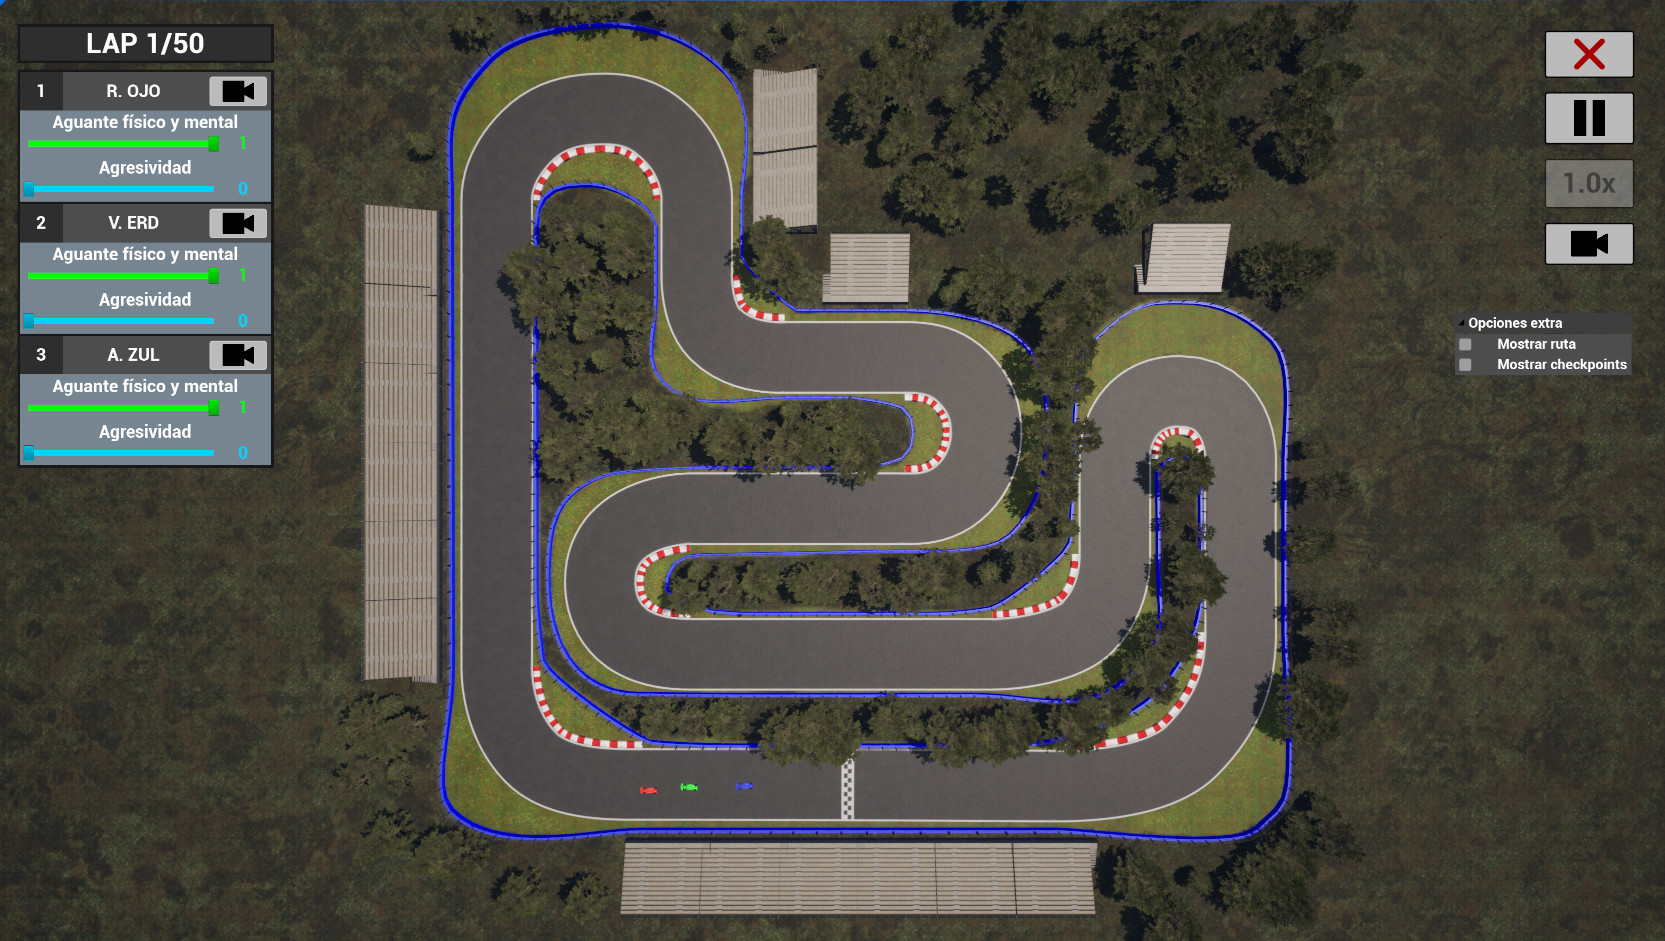
\includegraphics[width=\textwidth]{imagenes/camera/cam-top.jpg}
    \caption{Perspectiva cenital.}
    \label{fig:cenital}
\end{figure}

\begin{figure}[H]
    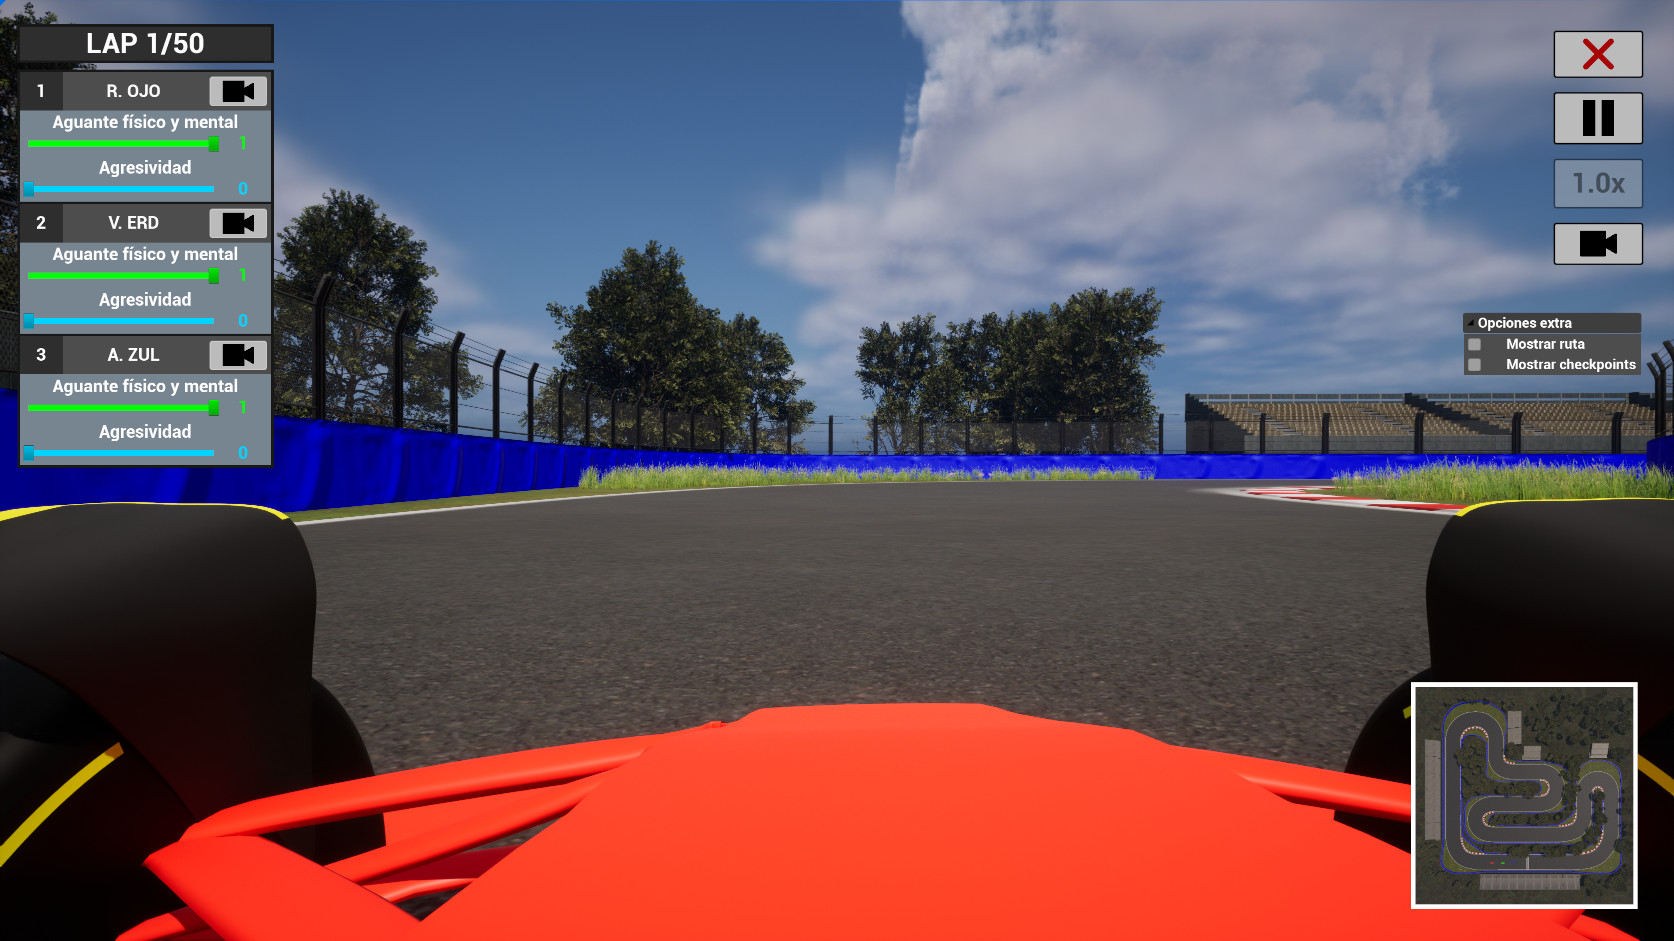
\includegraphics[width=\textwidth]{imagenes/camera/cam-frontal.jpg}
    \caption{Perspectiva frontal del vehículo.}
    \label{fig:frontal}
\end{figure}

\begin{figure}[H]
    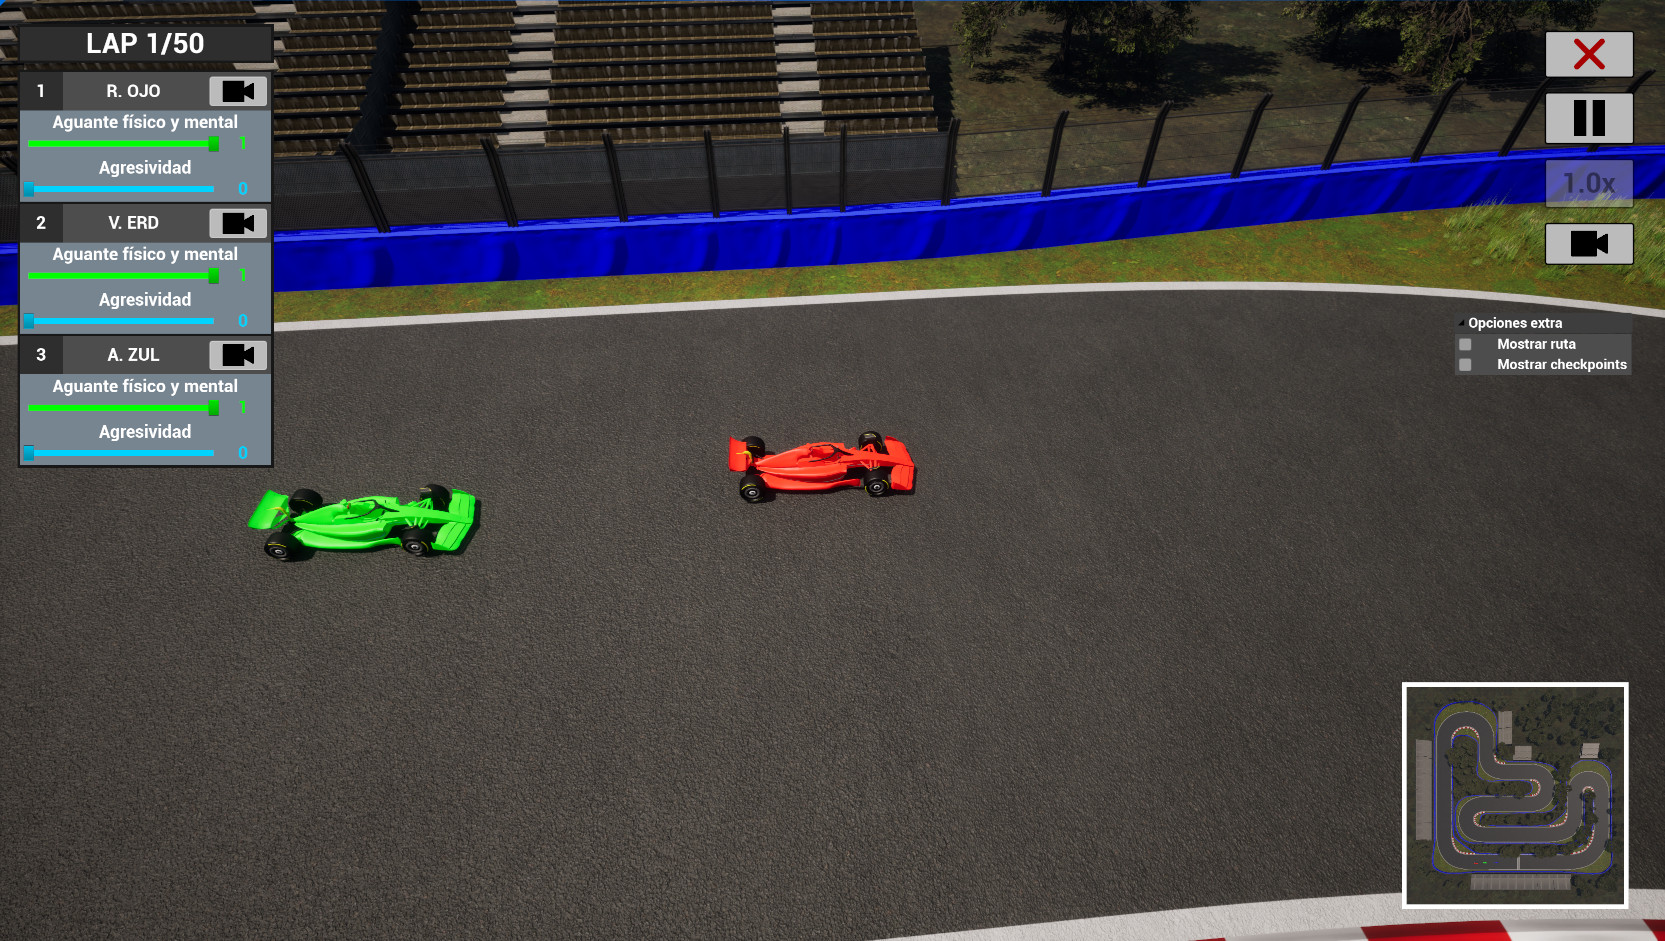
\includegraphics[width=\textwidth]{imagenes/camera/cam-pers.jpg}
    \caption{Perspectiva de diversas cámaras.}
    \label{fig:cam-estaticas}
\end{figure}

Para realizar el seguimiento con cámaras estáticas, he reutilizado el actor (glosario en la sección \ref{sec:terminosunreal}) ``SplinePath'', utilizada para crear las rutas del algoritmo A*, para crear un spline, cuyos puntos son las posiciones que puede tener la cámara. Después, he creado el actor ``CameraFollower'', que tiene una referencia a todos los vehículos, de forma que elige cada cierto tiempo uno al azar y calcula el punto del spline más cercano al coche. Finalmente, mueve la cámara a dicho punto y la rota para que apunte en cada momento al coche.

\bigskip

En las figuras \ref{fig:bp-cam1} y \ref{fig:bp-cam2} se encuentra la implementación de la obtención del punto del spline y el movimiento de la cámara al objetivo, respectivamente:

\begin{figure}[H]
    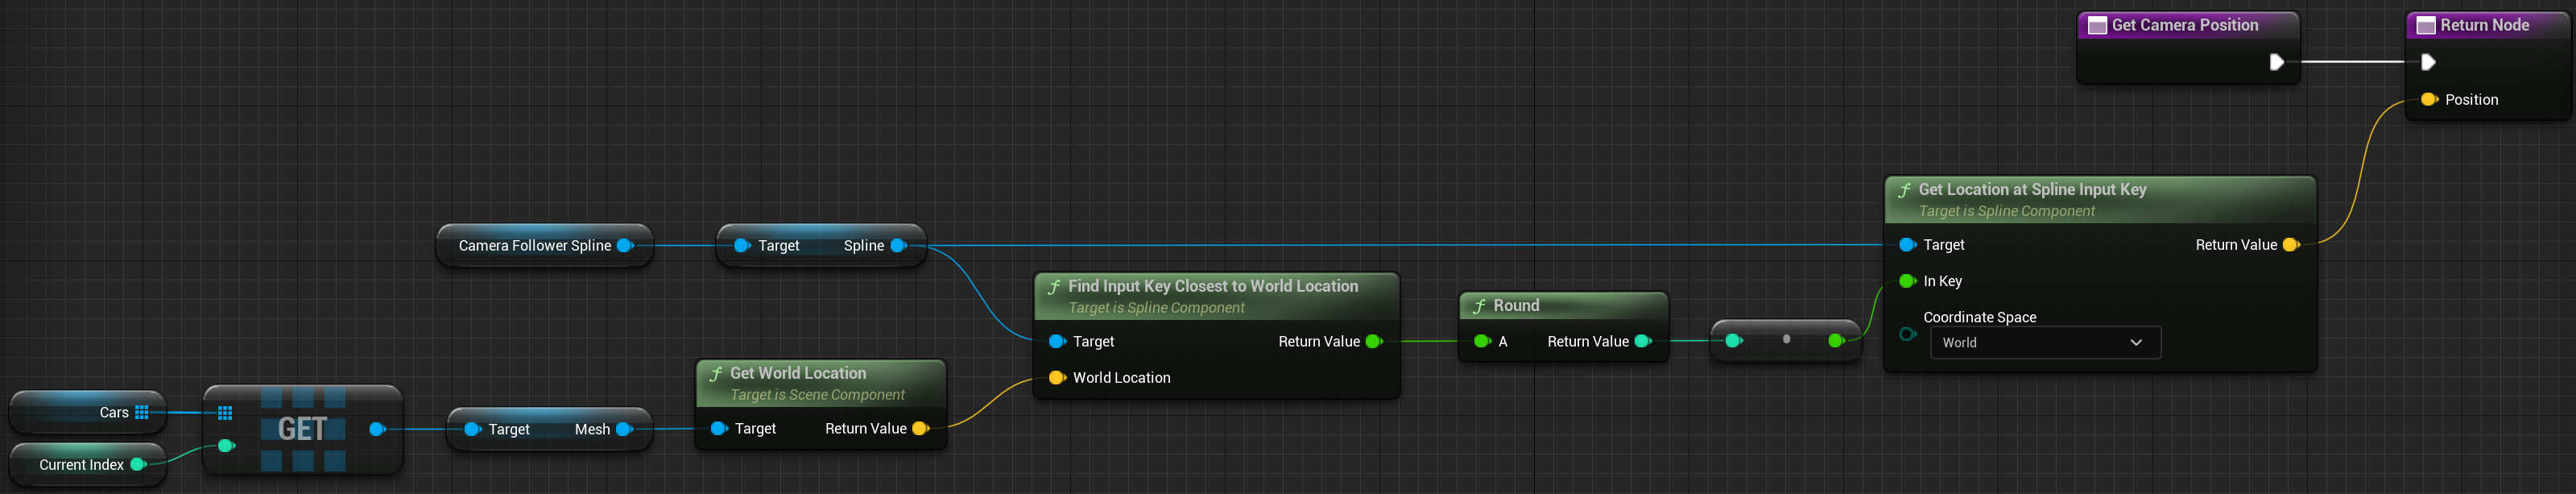
\includegraphics[width=\textwidth]{imagenes/blueprints/CameraFollower.getCameraPosition.png}
    \caption{Implementación de la obtención del punto del spline.}
    \label{fig:bp-cam1}
\end{figure}

\begin{figure}[H]
    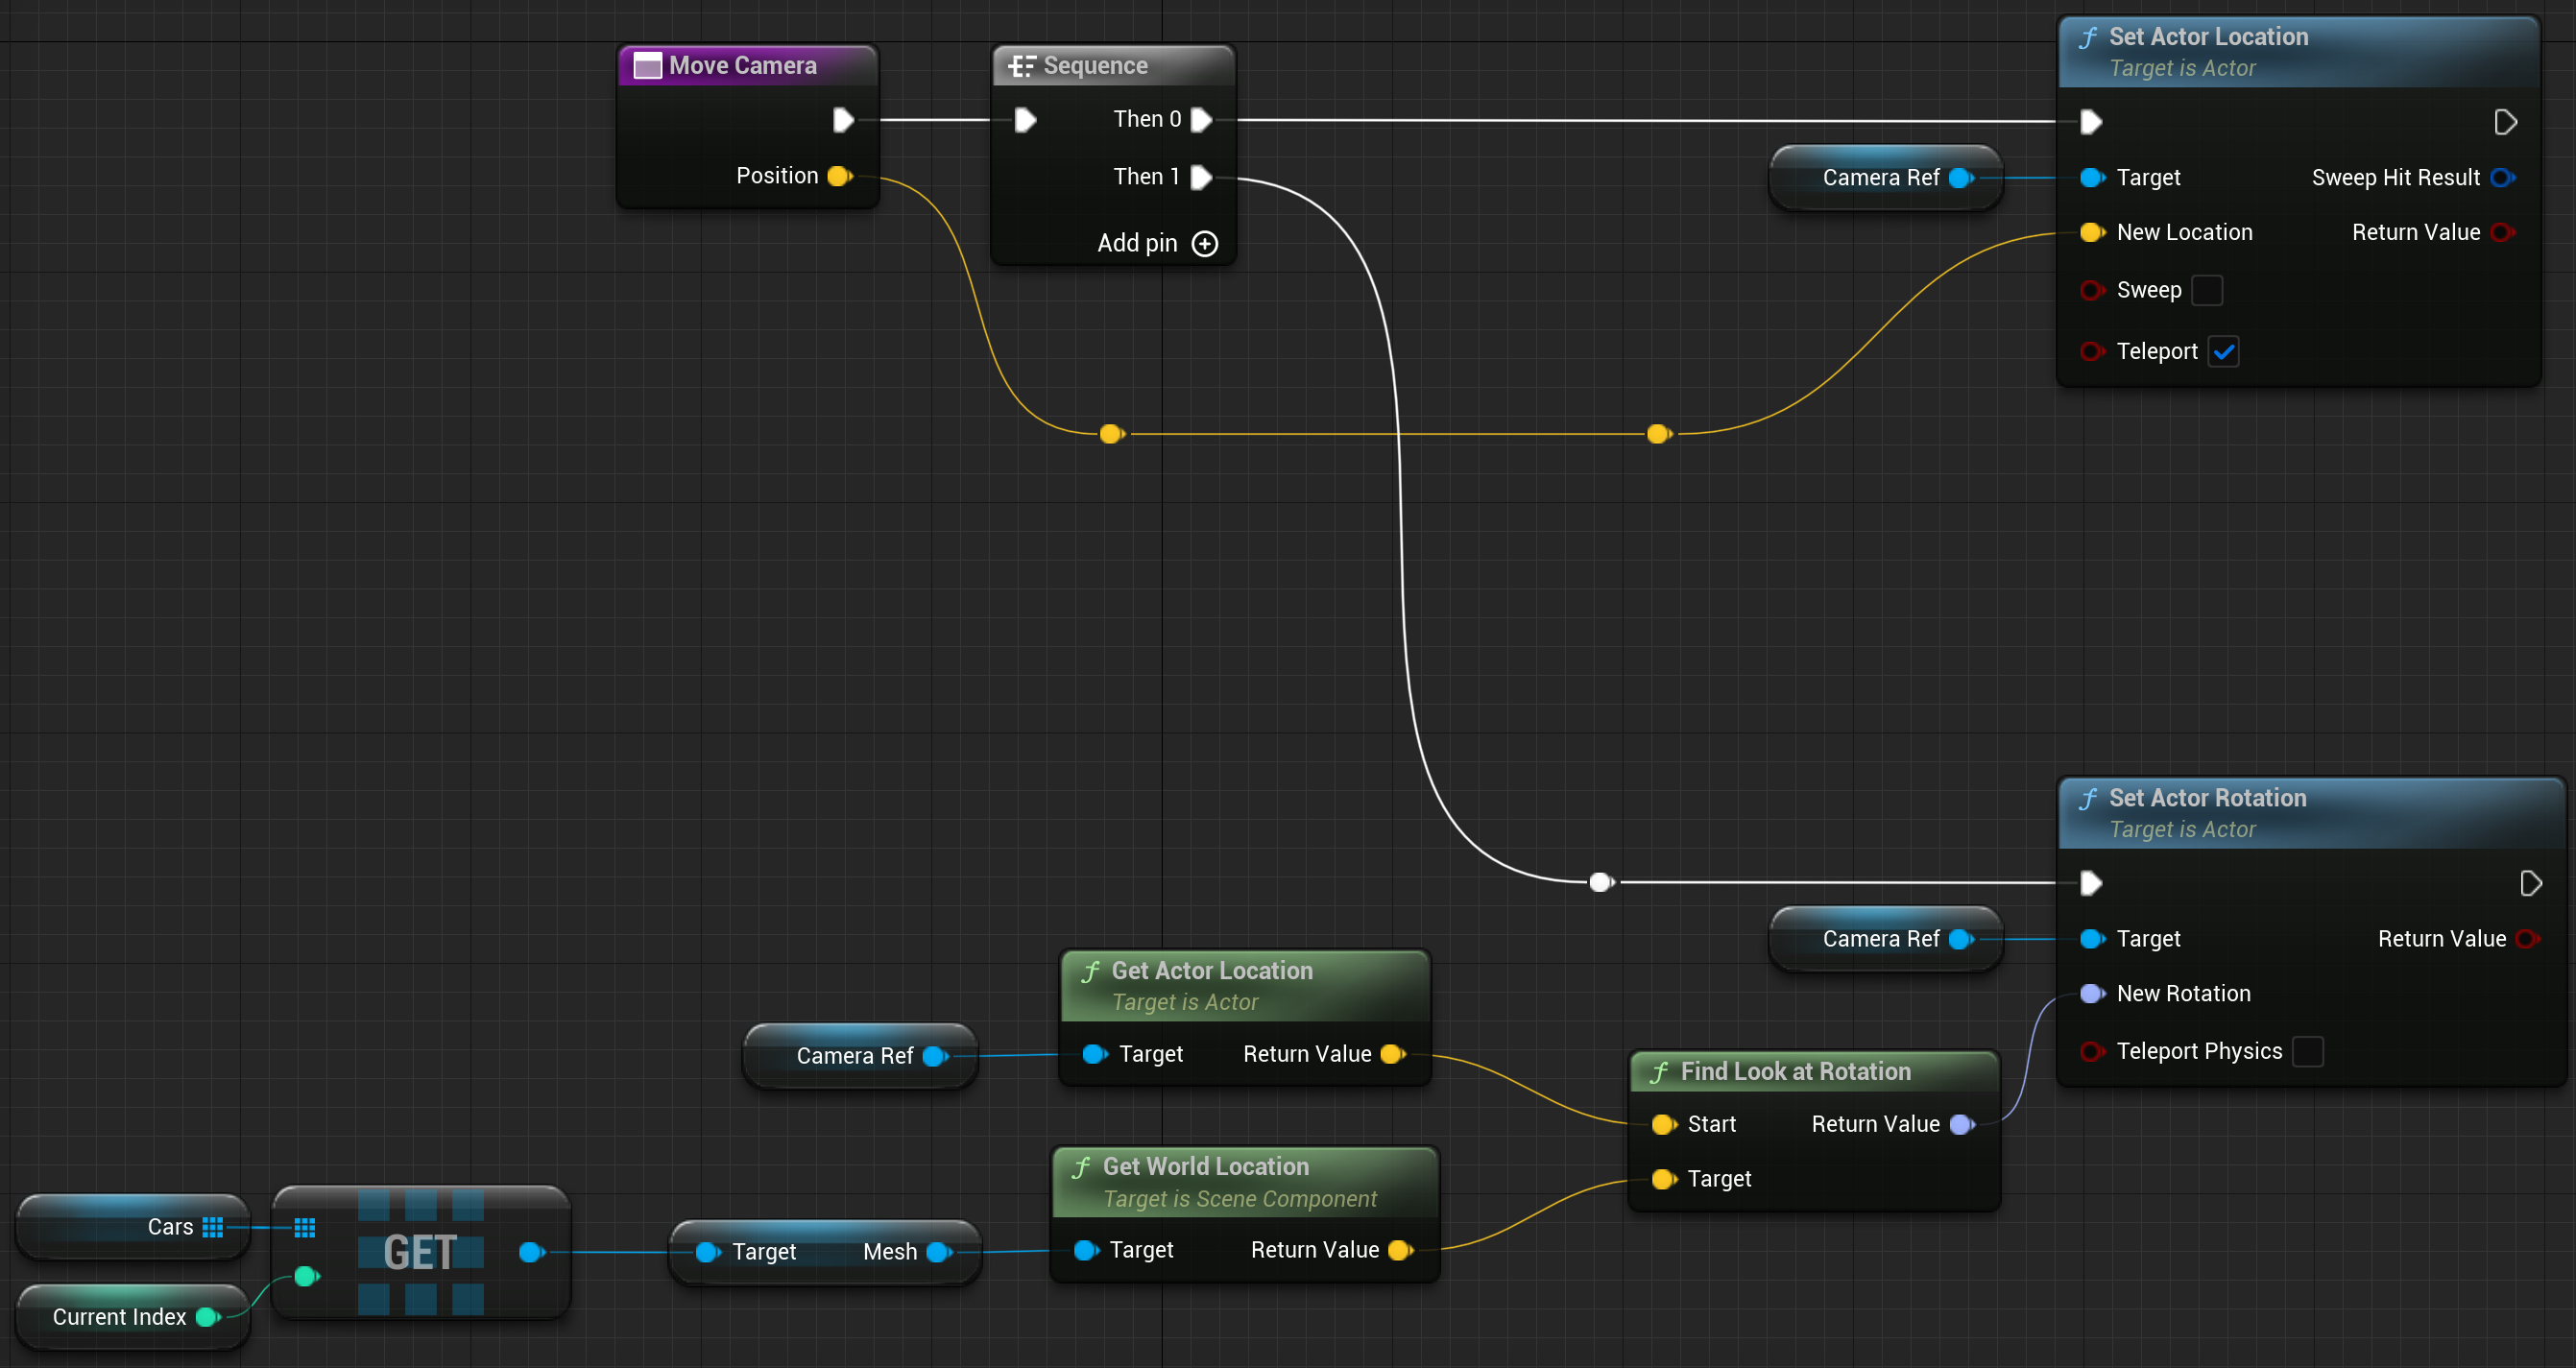
\includegraphics[width=\textwidth]{imagenes/blueprints/CameraFollower.moveCamera.png}
    \caption{Implementación del posicionamiento de la cámara.}
    \label{fig:bp-cam2}
\end{figure}

\subsubsection{Enmarcado del objetivo}

Debido al amplio rango de relaciones de aspecto con las que la aplicación puede trabajar, es posible que el objetivo sea enmarcado demasiado lejos o incluso se llegue a cortar. Para solucionarlo, es necesario ajustar los valores del FOV \textit{(Field Of View)} para que siempre se mantenga enmarcado. La modificación del FOV se realiza mediante una función lineal basada en los valores de FOV más coherentes para las relaciones de aspecto 1:1 y 21:9 y un ajuste manual de las constantes de la función. 

\bigskip

La función final es: $f(x) = 34.5865 \cdot x + 26.4135$, donde $x$ representa la relación de aspecto en formato numérico (diviendo ambos valores). Además, la he encapsulado en la clase ``CameraHandler'', para que los coches también puedan utilizar sus métodos.

\subsection{Cálculo de la zona de frenado}

Los coches necesitan saber en qué instante frenar para poder tomar las curvas sin salirse de pista. Con este fin, deben conocer la distancia al siguiente checkpoint donde deben comenzar a frenar.

\bigskip

He calculado la distancia de frenado utilizando la fórmula del MRUA (Movimiento Rectilíneo Uniformemente Acelerado) y despejando la distancia.

\bigskip

Partiendo de las fórmulas siguientes: 

$d = d_0 + v_0 \cdot t + \frac{1}{2} \cdot a \cdot t$

$v = v_0 + a \cdot t$

\bigskip

Al despejar la variable $t$ en la segunda fórmula y sustituirla en la primera, se procede a simplificar la expresión obteniendo: $ d = \frac{v^2-v_0^2}{2 \cdot a} $, donde $a$ es la deceleración, $v$ la velocidad a la que se quiere llegar y $v_0$ la velocidad actual.

\bigskip

Cabe destacar que la deceleración la he obtenido mediante el uso de otros vehículos con las mismas características que los utilizados en las carreras, pero con la capacidad de ser controlados con el teclado. Después, he calculado el valor G de la deceleración, el cual, al multiplicarlo por la gravedad, resulta en el valor final.
% de forma que multiplicado por la gravedad obtenga el valor final.

\section{Modelado y texturizado de la escena}

Para la creación, preparación y modificación de los distintos modelos y texturas de la aplicación, he utilizado Blender\cite{blender} y GIMP\cite{gimp}. A continuación detallaré cada uno de los modelos y texturas, así como su proceso de creación.

\subsection{Trazado del circuito}

El trazado de la carretera lo he realizado creando primero un spline en Unreal con la forma deseada. A continuación, se debe incluir un modelo de carretera para que el spline pueda generarlo siguiendo la forma del trazado.
\begin{figure}[H]
    \centering
    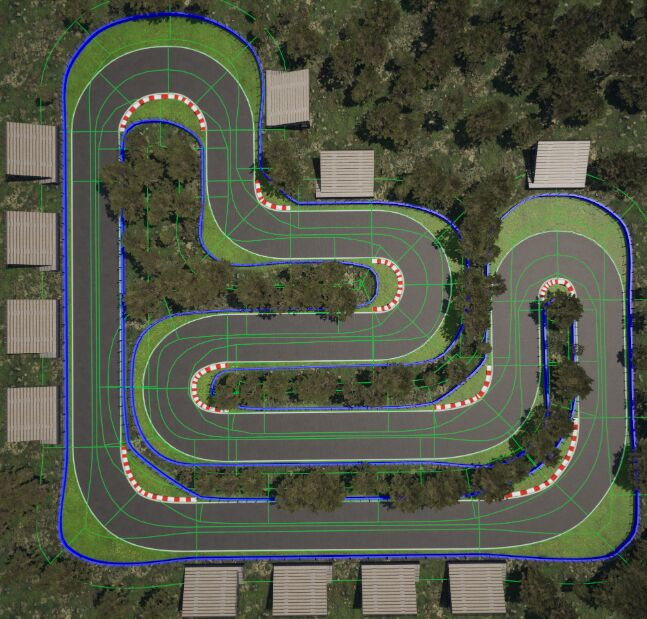
\includegraphics[width=0.7\textwidth]{imagenes/converted/trazadoFinal.jpg}
    \caption{Trazado del circuito final.}
    \label{fig:trazado}
\end{figure}


En la vida real, los circuitos suelen tener secciones donde la carretera es recta y otras secciones donde se incluyen pianos, especialmente en las curvas. Por lo tanto, ha sido necesario crear tres modelos distintos de pista: uno sin piano, otro con piano a la izquierda y otro con el piano a la derecha. De esta manera, se logra una representación más fiel y realista de las diferentes secciones del circuito.

\bigskip

He utilizado Blender para generar los tres modelos de pista. Las secciones se construyeron a partir de un cubo achatado, y en las versiones con piano, se ha extruido uno de los lados y se ha aplicado un \textit{bevel} para suavizar las esquinas.

% fotos de las 3 versiones
\begin{figure}[H]
    \centering
    \begin{subfigure}[t]{0.48\textwidth}
        \centering
        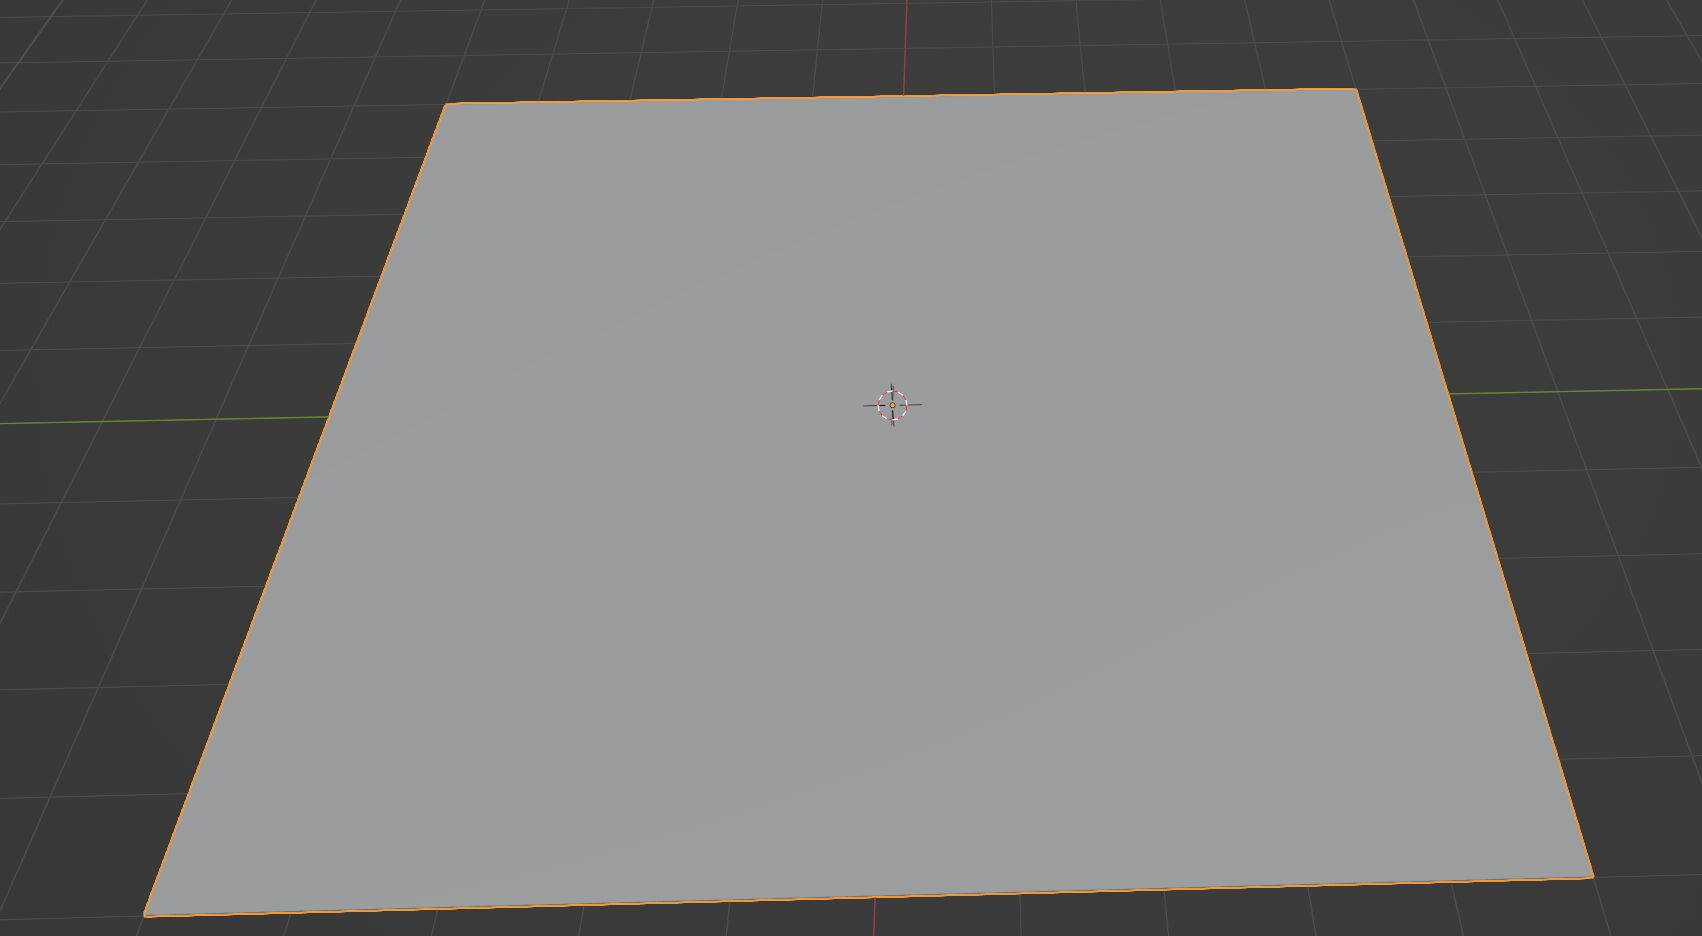
\includegraphics[width=\textwidth]{imagenes/converted/pista/curva-recta.jpg}
        \caption{Sección recta de la curva.}
        \label{fig:curvarecta}
    \end{subfigure}
    \hfill
    \begin{subfigure}[t]{0.48\textwidth}
        \centering
        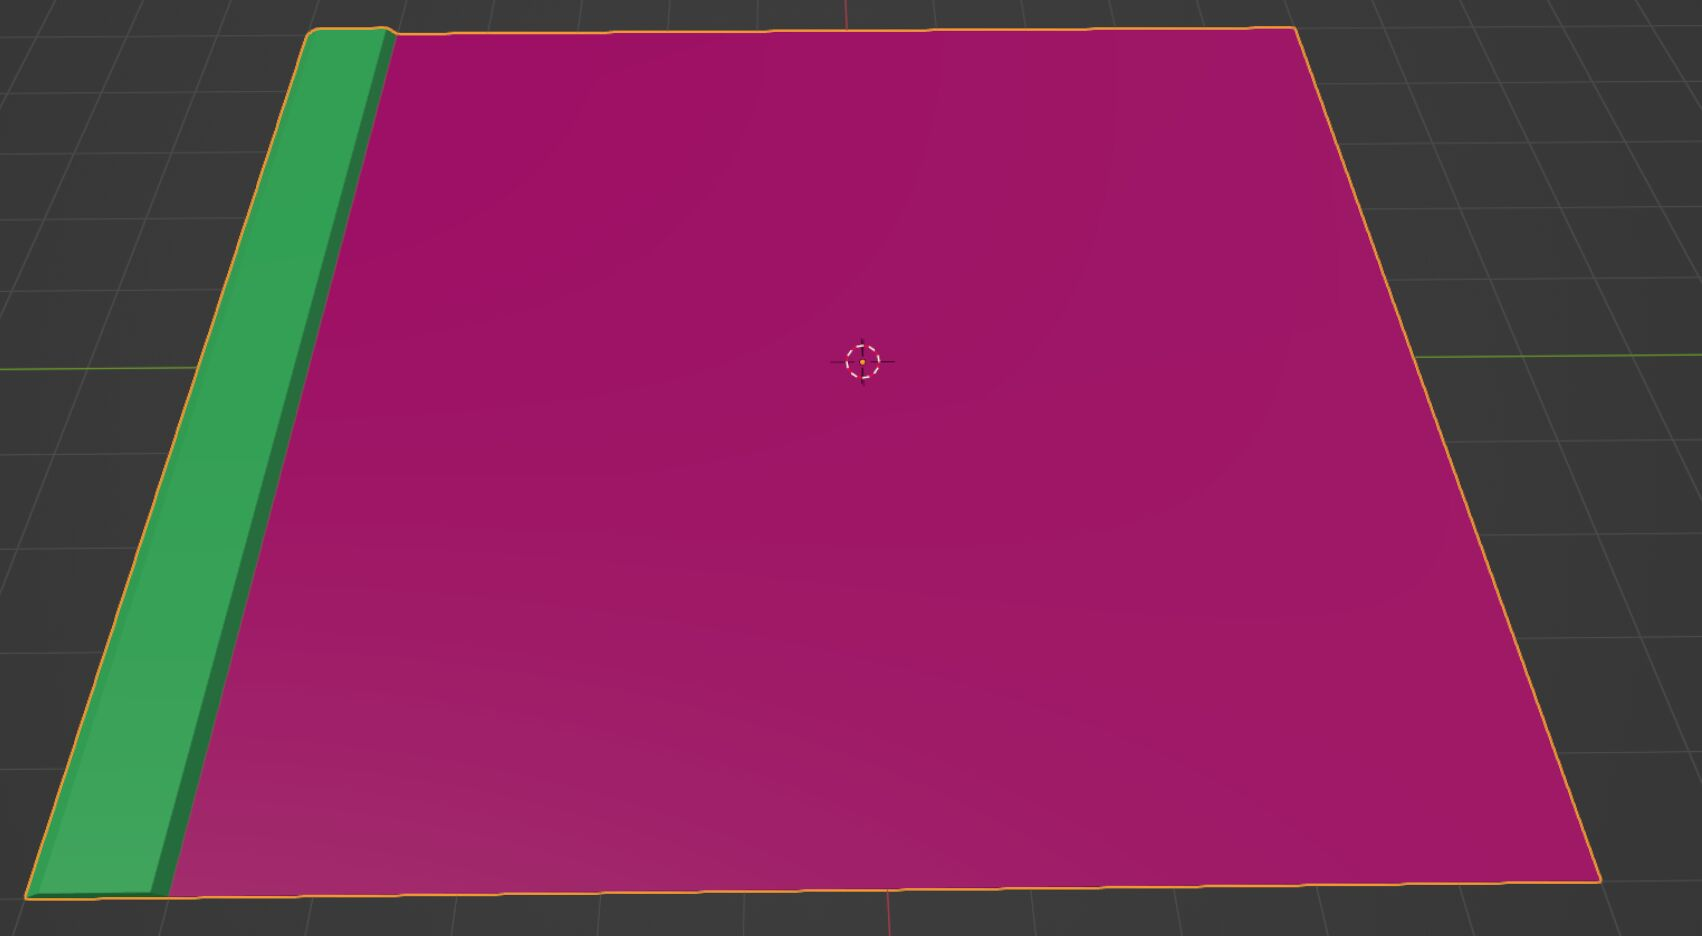
\includegraphics[width=\textwidth]{imagenes/converted/pista/curva.jpg}
        \caption{Sección con el piano a la izquierda.}
        \label{fig:curvaL}
    \end{subfigure}
    \par\bigskip
    \begin{subfigure}[t]{0.48\textwidth}
        \centering
        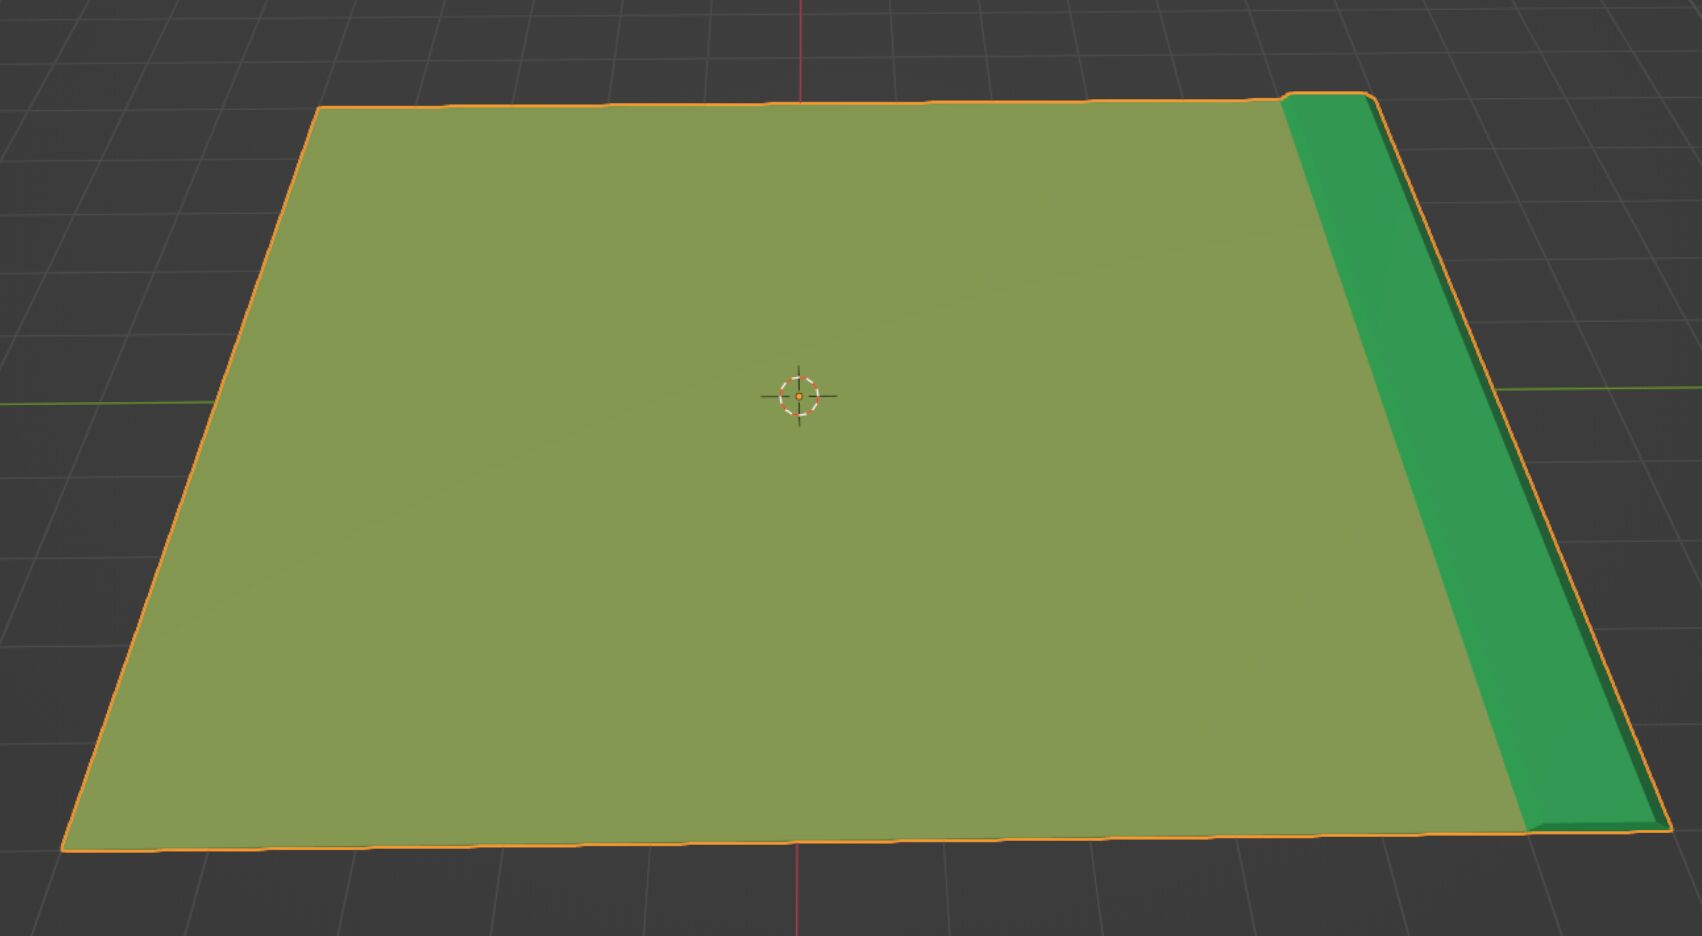
\includegraphics[width=\textwidth]{imagenes/converted/pista/curva-inverted.jpg}
        \caption{Sección con el piano a la derecha.}
        \label{fig:curvaR}
    \end{subfigure}
    \caption{Modelos de pista utilizados.}
    \label{fig:curvasmodelos}
\end{figure}

Después, he utilizado la textura ``Asphalt 024 A''\cite{asphalt}, creada por Lennart Demes, y he modificado la componente difusa utilizando GIMP para poner una línea continua a ambos extremos, similar a los circuitos reales. Adicionalmente, he modificado la textura con las dos líneas para añadirle una sección con la línea de meta. En la figura \ref{fig:asfaltoTextura} se pueden observar ambas texturas.

\begin{figure}[H]
    \centering 
	\begin{subfigure}[t]{0.48\textwidth}
	    \centering
        
\includegraphics[width=0.98\textwidth,cframe=black 0.5pt 0pt]{imagenes/converted/pista/Asphalt024A_2K_Color.jpg}
        \caption{Textura de asfalto modificada.}
        \label{fig:asfaltomod}
    \end{subfigure}
    \hfill 
    %\par\bigskip %si se desea dejar un margen entre la imagen de arriba y de abajo. SOLO SE PUEDE USAR HFILL O ESTE
    %\hspace{10px} %si se quiere poner una medida personalizada
	\begin{subfigure}[t]{0.48\textwidth}
	    \centering
	    
\includegraphics[width=0.98\textwidth,cframe=black 0.5pt 0pt]{imagenes/converted/pista/Asphalt024A_2K_Color_FinishLineFinal.jpg}
        \caption{Textura de asfalto con la línea de meta.}
    \end{subfigure}    
    \caption{Texturas de asfalto utilizadas en la aplicación. Se han enmarcado para poder separar las imágenes del fondo de la página.}
    \label{fig:asfaltoTextura}
\end{figure}

Para texturizar el piano, he decidido crear la textura yo mismo. Utilizando GIMP, he creado una textura difusa con un tamaño de 2048x2048 píxeles y he pintado una mitad de color blanco y la otra de color rojo. 


\begin{figure}[H]
    \centering
    
\includegraphics[width=0.4\textwidth]{imagenes/converted/pista/kerb-dirty2.jpg}
    \caption{Textura utilizada para la componente difusa del piano.}
    \label{fig:pianodiff}
\end{figure}

El resultado en Unreal no era del todo convincente, ya que los bordes tenían demasiada iluminación. Para solucionarlo, he creado una textura para la componente de oclusión ambiental, de forma que los bordes sean algo más oscuros que la parte central. 

\begin{figure}[H]
    \centering
    
\includegraphics[width=0.4\textwidth,cframe=black 0.5pt 0pt]{imagenes/converted/pista/kerb-dirty2-AO.jpg}
    \caption{Textura utilizada para la oclusión ambiental del piano. Enmarcado para diferenciar del fondo de la página.}
    \label{fig:pianoao}
\end{figure}

Estas texturas no encajaban del todo bien, haciendo que las líneas blancas no estuviesen alineadas con los bordes y que la textura del piano no se repitiese varias veces en la sección. Utilizando Blender, he realizado un mapeado UV de los modelos, con el objetivo de que la asignación de las texturas se realice correctamente.

\begin{figure}[H]
    \centering
    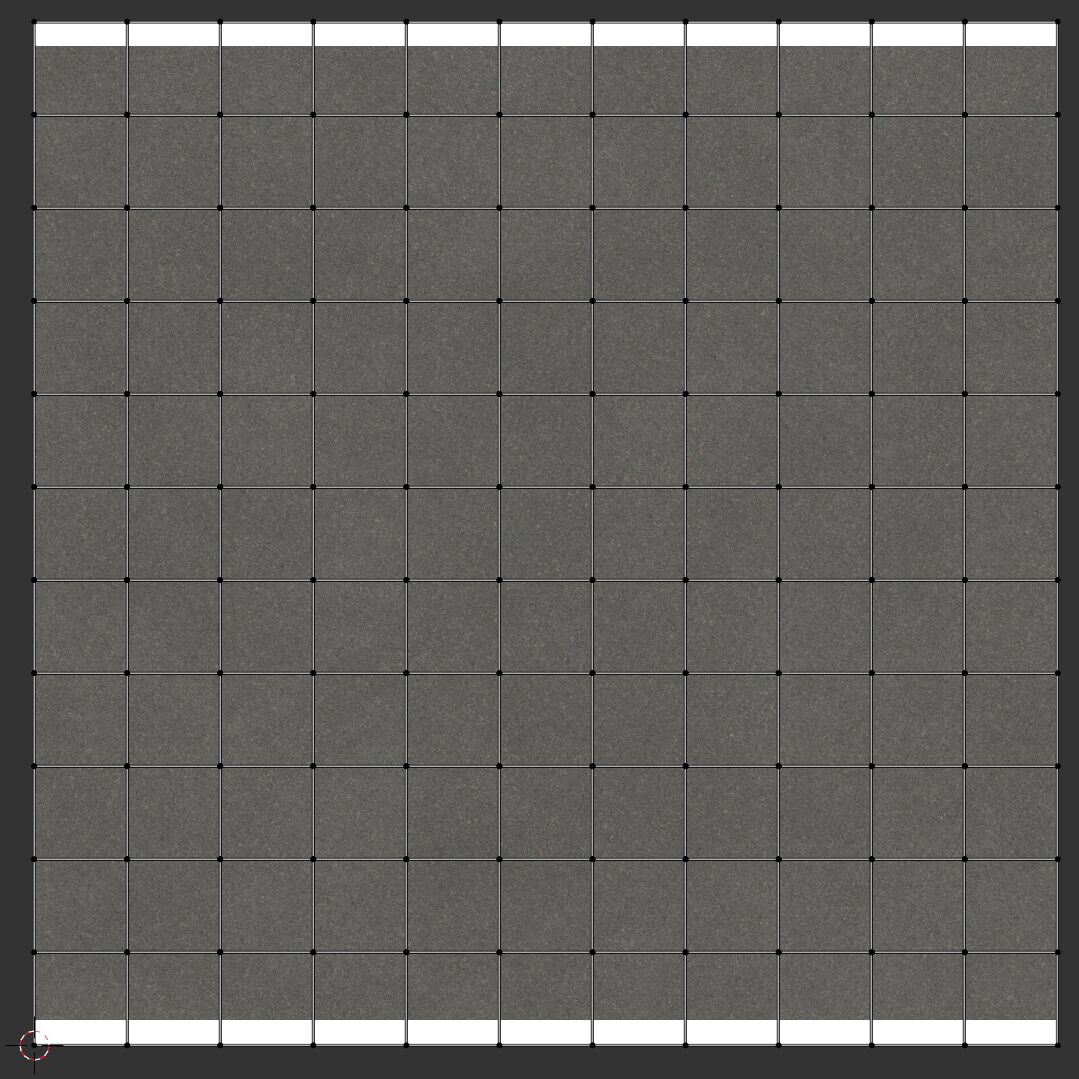
\includegraphics[width=0.4\textwidth]{imagenes/converted/pista/uv-straight.jpg}
    \caption{Mapeado UV para la sección de asfalto.}
    \label{fig:uvasphalt}
\end{figure}

\begin{figure}[H]
    \centering
    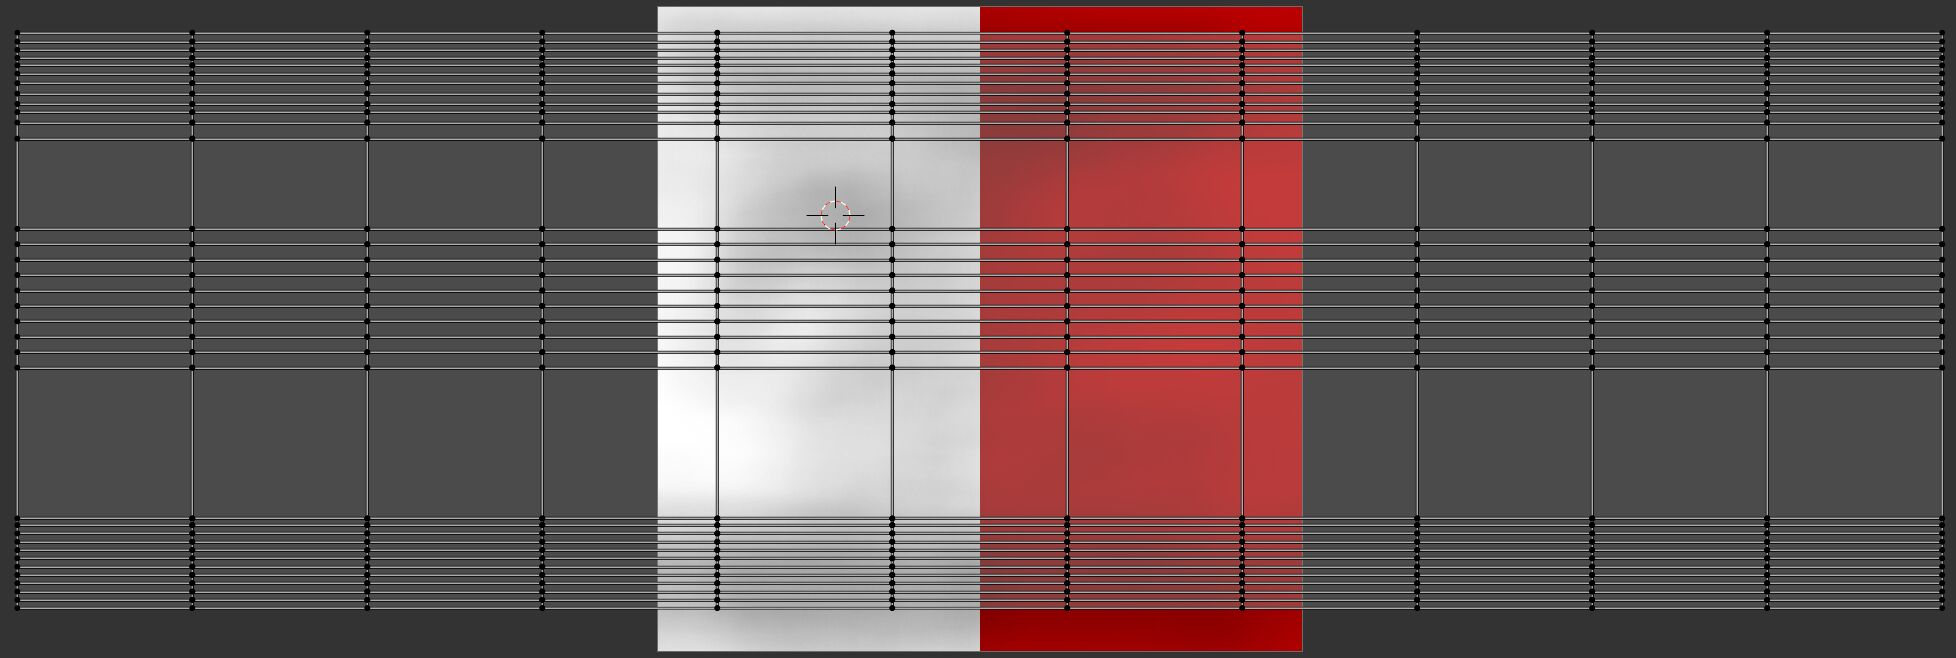
\includegraphics[width=0.8\textwidth]{imagenes/converted/pista/uv-kerb.jpg}
    \caption{Mapeado UV para la sección de piano.}
    \label{fig:uvkerb}
\end{figure}

Ahora sí se sitúan bien las texturas en el modelo. En la figura \ref{fig:seccionespista} se encuentra el resultado final en Unreal.

\begin{figure}[H]
    \centering
    \begin{subfigure}[t]{0.48\textwidth}
        \centering
        
\includegraphics[width=\textwidth]{imagenes/converted/pista/track-final.jpg}
        \caption{Sección de pista con el piano a la derecha.}
        \label{fig:curvafinal2}
    \end{subfigure}
    \hfill
    \begin{subfigure}[t]{0.48\textwidth}
        \centering
        
\includegraphics[width=\textwidth]{imagenes/converted/pista/track-final-inverted.jpg}
        \caption{Sección de pista con el piano a la izquierda.}
        \label{fig:curvafinal3}
    \end{subfigure}
    \par\bigskip
    \begin{subfigure}[t]{0.48\textwidth}
        \centering
        
\includegraphics[width=\textwidth]{imagenes/converted/pista/track-straight-final.jpg}
        \caption{Sección de pista recta.}
        \label{fig:curvafinal1}
    \end{subfigure}
    \hfill
    \begin{subfigure}[t]{0.48\textwidth}
        \centering
        
\includegraphics[width=\textwidth]{imagenes/converted/pista/track-finish-line-final.jpg}
        \caption{Sección de pista recta con la línea de meta.}
        \label{fig:curvafinishlinefinal}
    \end{subfigure}

    \caption{Secciones de pista finales en Unreal.}
    \label{fig:seccionespista}
\end{figure}

\newpage

\subsection{Preparación de los coches}

Debido a que modelar un vehículo requiere demasiado tiempo, he optado por utilizar el modelo ``Porsche 911 GT3''\cite{porsche} realizado por ``ChevroletSS'' y el modelo ``Mercedes F1 W14''\cite{f1} realizado por ``3dblenderlol''. Además, he eliminado toda clase de logotipos y marcas de los vehículos, para facilitar la exportación.

\bigskip

A continuación, es necesario preparar los modelos para que las ruedas se puedan mover en Unreal. Se debe realizar un \textit{rigging} de las ruedas; es decir, asignarle un conjunto de huesos, que actuarán como ejes para la rotación de las mismas. Esta tarea la he realizado cargando los modelos y utilizando el plugin de Blender ``UE4 Vehicle Rigging Addon for Blender''\cite{blenderplugin}, creado por ``Continue Break''. El plugin permite realizar el \textit{rigging} de manera automática con tan solo indicarle el chasis del coche y sus ruedas.

\begin{figure}[H]
    \centering
\begin{subfigure}[t]{0.48\textwidth}
    \centering
    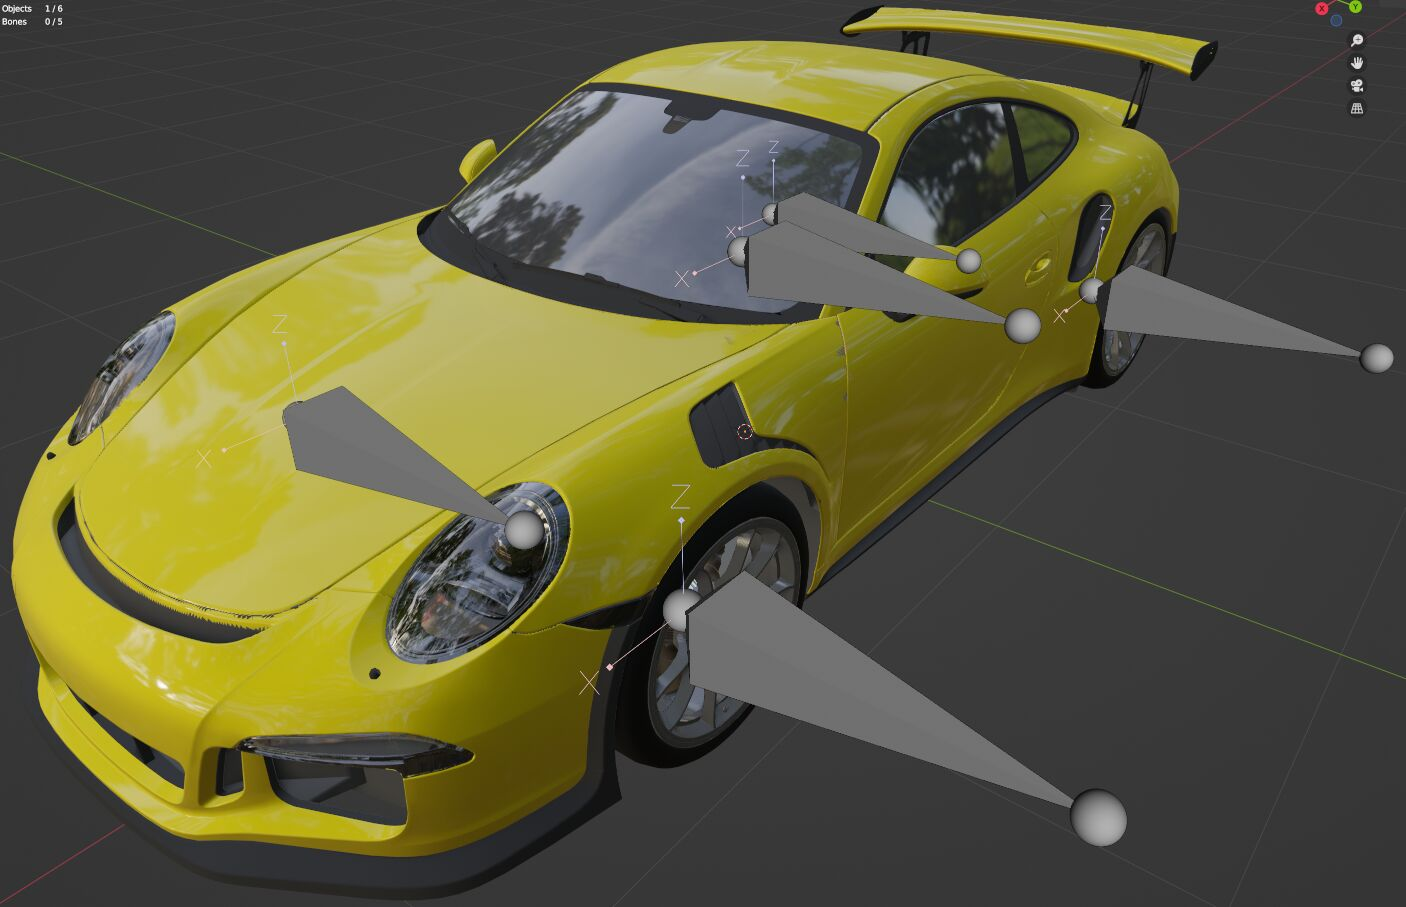
\includegraphics[width=\textwidth]{imagenes/converted/rigging/911-rigging.jpg}
    \caption{\textit{Rigging} realizado en el Porsche 911.}
    \label{fig:rigging911}
\end{subfigure}
\hfill
\begin{subfigure}[t]{0.48\textwidth}
    \centering
    % \includegraphics[width=\textwidth]{imagenes/trazado.jpg}
    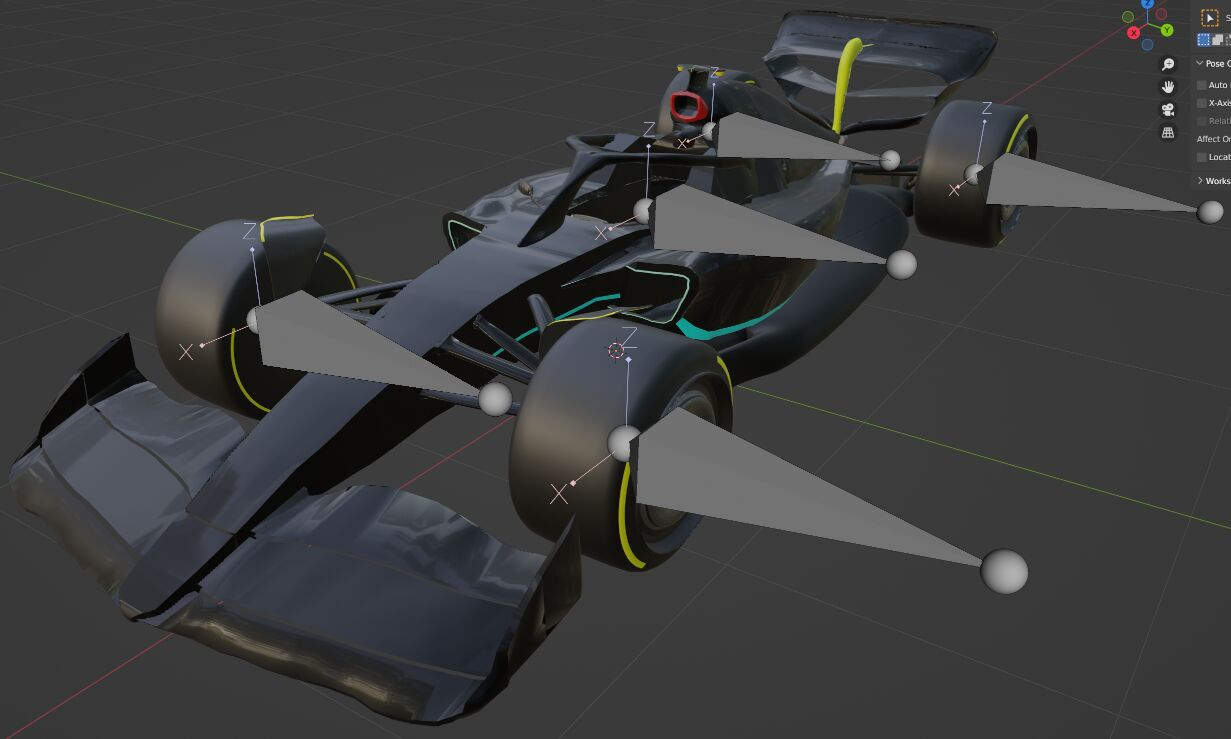
\includegraphics[width=\textwidth]{imagenes/converted/rigging/f1-rigging.jpg}
    \caption{\textit{Rigging} realizado en el coche de Fórmula 1.}
    \label{fig:riggingf1}
\end{subfigure}
\caption{\textit{Rigging} de los vehículos.}
\end{figure}

Así, ya se tendría realizado el \textit{rigging} de los vehículos. Ahora es necesario importarlos, crear sus animaciones y \textit{bounding boxes} para que funcione correctamente.

\newpage

\subsection{Barreras}

Es necesario establecer los límites del circuito mediante barreras similares a las utilizadas en los circuitos reales. Para ello, he decidido utilizar el modelo de valla ``3D Model Metal Fence''\cite{fence}, creado por ``Adrian Kulawik'', junto a un modelo de barrera creado por mí en Blender.

\bigskip

Debido a que quería simular que mi barrera está algo arrugada, como pasa en la vida real, he utilizado \textit{Sculpt Mode} para esculpir las diversas imperfecciones en un modelo de alta resolución. 

\begin{figure}[H]
    \centering
    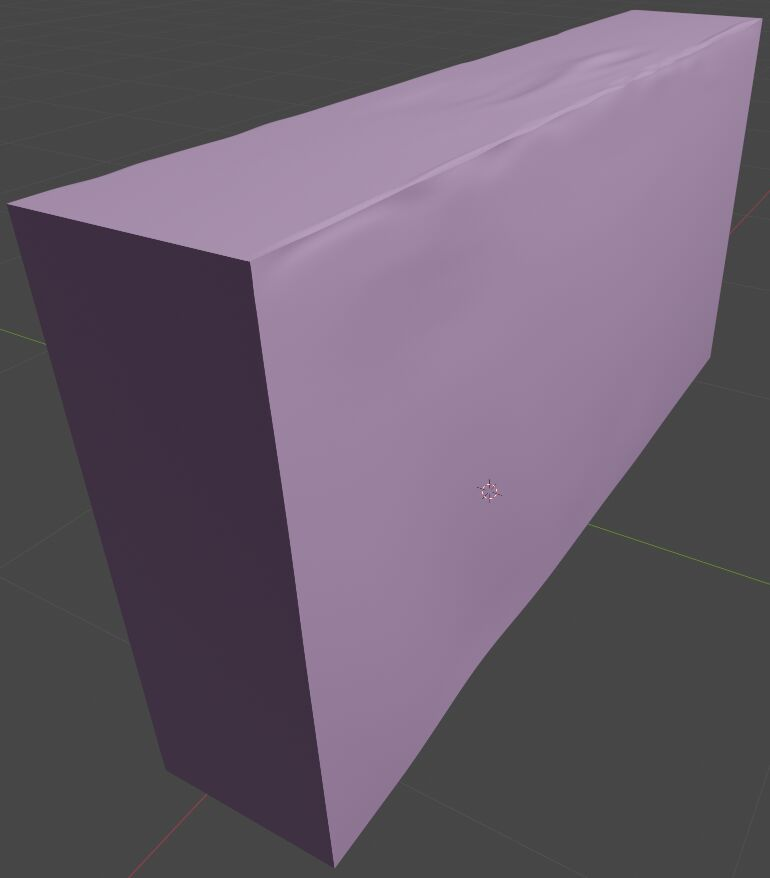
\includegraphics[width=0.4\textwidth]{imagenes/converted/barrier/barrierHP.jpg}
    \caption{Barrera de alta resolución con imperfecciones.}
    \label{fig:barreraHP}
\end{figure}

Como puede consumir demasiados recursos, he convertido las deformaciones geométricas en una textura normal utilizando Blender, de manera que se pueda poner sobre una versión simple de la barrera.

\begin{figure}[H]
    \centering
    \includegraphics[width=0.4\textwidth]{imagenes/converted/barrier/barrierNormal.jpg}
    \caption{Textura normal generada para la versión con pocos polígonos.}
    \label{fig:barreraLP}
\end{figure}


Y el modelo final es mi barrera, junto a la valla anteriormente mencionada encima.

\begin{figure}[H]
    \centering
    \includegraphics[width=0.4\textwidth]{imagenes/converted/barrier/barrierfence.jpg}
    \caption{Resultado final de la barrera en Unreal.}
    \label{fig:barreraFinal}
\end{figure}

Para que la barrera rodee todo el circuito, se sigue un procedimiento similar al del trazado. Se utiliza un spline que marca el recorrido y, luego, se asigna una barrera a cada sección del spline.

\newpage

\subsection{Vegetación}

La vegetación del circuito está compuesta por césped en las curvas y por árboles en el exterior y zonas intermedias del circuito. El modelo de césped utilizado ha sido ``temperate Vegetation: optimized Grass Library''\cite{grass}, creado por ``Project Nature'', y el de los árboles es ``Megascans Trees: European Black Alder (early access)''\cite{trees}, creado por ``Quixel Megascans''.

\bigskip

El resultado final es el siguiente:

% fotos de cerca de arboles y cesped
\begin{figure}[H]
    \centering
    \includegraphics[width=0.9\textwidth]{imagenes/converted/cesped.jpg}
    \caption{Modelo de césped.}
    \label{fig:cesped}
\end{figure}

\begin{figure}[H]
    \centering
    \includegraphics[width=0.9\textwidth]{imagenes/converted/arboles.jpg}
    \caption{Modelo de árboles.}
    \label{fig:arboles}
\end{figure}

\subsection{Modelos y texturas adicionales}

% rescribir
He utilizado la textura de césped ``Ground 037''\cite{grasstexture}, creada por ``Lennart Demes'', para las zonas en las que se puso el modelo tridimensional de césped (modelo 3D en figura \ref{fig:cesped}), con el objetivo de dar más realismo en distancias más lejanas, donde el modelo tridimensional no se aprecia. 

\bigskip

Para evitar el efecto \textit{tiling}, he interpolado el color de la textura en dos tonos ligeramente diferentes mediante un patrón de variación. Además, he utilizado otro patrón de variación para incluir zonas oscuras en el césped. En la figura \ref{fig:grasstexture} se puede ver la textura utilizada y en la figura \ref{fig:grassfinal} el resultado final.

\begin{figure}[H]
    \centering
    % \includegraphics[width=\textwidth]{imagenes/trazado.jpg}
    \includegraphics[width=0.4\textwidth]{imagenes/converted/Ground037_1K_Color.jpg}
    \caption{Componente difusa de la textura de césped utilizada.}
    \label{fig:grasstexture}
\end{figure}

\begin{figure}[H]
    \centering
    % \includegraphics[width=\textwidth]{imagenes/trazado.jpg}
    \includegraphics[width=0.4\textwidth]{imagenes/converted/cespedTextFinal}
    \caption{Resultado final del césped en Unreal.}
    \label{fig:grassfinal}
\end{figure}

Para la zona de los alrededores del circuito, he utilizado la textura ``Coast Sand Rocks 02''\cite{coastsand}, creada por ``Rob Tuytel'', aplicándole el mismo tratamiento que al césped. Los resultados de utilizar solo esta textura no eran del todo convincentes, por lo que he decidido mezclarla con la textura ``Ground 066''\cite{ground066}, creada por ``Lennart Demes''. De esta forma he obtenido un buen resultado, sin apreciarse \textit{tiling}. En la figura \ref{fig:exterior} se pueden ver las texturas utilizadas y en la figura \ref{fig:sueloFinal} el resultado final:.

% Además, se ha hecho uso de la textura ``Coast Sand Rocks 02''\cite{coastsand}, creada por ``Rob Tuytel'', para el suelo del exterior del circuito, donde se encuentran los árboles (modelo 3D en figura \ref{fig:arboles}).

\begin{figure}[H]
    \centering 
	\begin{subfigure}[t]{0.48\textwidth}
	    \centering
        \includegraphics[width=\textwidth]{imagenes/converted/coast_sand_rocks_02_diff_4k.jpg}
        \caption{Componente difusa de la textura tierra y hierba del suelo.}
        \label{fig:coastsand}
    \end{subfigure}
    \hfill 
    %\par\bigskip %si se desea dejar un margen entre la imagen de arriba y de abajo. SOLO SE PUEDE USAR HFILL O ESTE
    %\hspace{10px} %si se quiere poner una medida personalizada
	\begin{subfigure}[t]{0.48\textwidth}
	    \centering
        \includegraphics[width=\textwidth]{imagenes/converted/Ground066_2K_Color.jpg}
        \caption{Componente difusa de la textura de tierra del suelo.}
        \label{fig:ground066}
    \end{subfigure}    
    \caption{Texturas utilizadas para el suelo exterior.}
    \label{fig:exterior}
\end{figure}

\begin{figure}[H]
    \centering
    % \includegraphics[width=\textwidth]{imagenes/trazado.jpg}
    \includegraphics[width=0.5\textwidth]{imagenes/converted/sueloTextFinal}
    \caption{Representación final del suelo.}
    \label{fig:sueloFinal}
\end{figure}

Por último, se ha utilizado el modelo ``Grand stand 3d model''\cite{grandstand}, creado por ``VT Studios'', para incluir algunas gradas en los alrededores del circuito.

\begin{figure}[H]
    \centering
    % \includegraphics[width=\textwidth]{imagenes/trazado.jpg}
    \includegraphics[width=\textwidth]{imagenes/converted/grandstand.jpg}
    \caption{Modelo de las gradas utilizadas.}
    \label{fig:grandstand}
\end{figure}

% ################################ FIN MIS CAPITULOS ################################
%\input{capitulos/01_Introduccion}
%
%\input{capitulos/02_EspecificacionRequisitos}
%
%\input{capitulos/03_Planificacion}
%
%\input{capitulos/04_Analisis}
%
%\input{capitulos/05_Diseno}
%
%\input{capitulos/06_Implementacion}
%
%\input{capitulos/07_Pruebas}
%
%\input{capitulos/08_Conclusiones}
%
%%\chapter{Conclusiones y Trabajos Futuros}
%
%
%%\nocite{*}
\bibliography{bibliografia/bibliografia}\addcontentsline{toc}{chapter}{Bibliografía}
% \bibliographystyle{miunsrturl}
\bibliographystyle{plainurl}
%
%\appendix
%\input{apendices/manual_usuario/manual_usuario}
%%\input{apendices/paper/paper}
%\input{glosario/entradas_glosario}
% \addcontentsline{toc}{chapter}{Glosario}
% \printglossary
\chapter*{}
\thispagestyle{empty}

\end{document}
